\documentclass[titlepage, fleqn, a4paper, 12pt, twoside]{article}
\usepackage{exsheets} %question and solution environments
\usepackage{amsmath, amssymb, amsthm} %standard AMS packages
\usepackage[utf8]{inputenc}
\usepackage{esint} %integral signs
\usepackage{marginnote} %marginnotes
\usepackage{gensymb} %miscellaneous symbols
\usepackage{commath} %differential symbols
\usepackage{xcolor} %colours
\usepackage{cancel} %cancelling terms
\usepackage[free-standing-units,space-before-unit]{siunitx} %formatting units
	\sisetup
	{
		per-mode=fraction,
		fraction-function=\frac
	}
\usepackage{tikz, pgfplots} %diagrams
	\usetikzlibrary{calc, hobby, patterns, intersections, angles, quotes, spy}
\usepackage{graphicx} %inserting graphics
\usepackage{epstopdf} %converting and inserting eps graphics
\usepackage{hyperref} %hyperlinks
\usepackage{datetime} %date and time
\usepackage{ulem} %underline for \emph{}
\usepackage{xfrac, lmodern} %inline fractions
\usepackage{enumerate, enumitem} %numbered lists
\usepackage{float} %inserting floats
\usepackage[american voltages]{circuitikz} %circuit diagrams
\usepackage{pdflscape} %pages in landscape orientation
\usepackage{setspace} %double spacing
\usepackage{microtype} %micro-typography
\usepackage{listings} %formatting code
	\lstset{language=Matlab}
	\lstdefinestyle{standardMatlab}
	{
		belowcaptionskip=1\baselineskip,
		breaklines=true,
		frame=L,
		xleftmargin=\parindent,
		language=C,
		showstringspaces=false,
		basicstyle=\footnotesize\ttfamily,
		keywordstyle=\bfseries\color{green!40!black},
		commentstyle=\itshape\color{purple!40!black},
		identifierstyle=\color{blue},
		stringstyle=\color{orange},
	}
\usepackage{algpseudocode} %algorithms
\usepackage{algorithm} %algorithms
\usepackage{chronology}
\usepackage{qtree}
\usepackage{varwidth}
\usepackage{asymptote}
\usepackage{chemfig}
\usepackage{booktabs}
\usepackage{multirow}
\usepackage{titlesec}
\usepackage{todonotes}
\usepackage{ifdraft}
	\ifoptiondraft
	{%
		\doublespacing
		\usepackage{showframe}
	}
	{%
	    % nothing to be done here
	}

\newcommand\numberthis{\addtocounter{equation}{1}\tag{\theequation}} %adds numbers to specific equations in non-numbered list of equations

\theoremstyle{definition}
\newtheorem{example}{Example}
\newtheorem{definition}{Definition}

\theoremstyle{theorem}
\newtheorem{theorem}{Theorem}
\newtheorem{law}{Law}

\newcommand{\curl}{\mathrm{curl\,}}

\newcommand{\divergence}{\mathrm{div\,}}

\DeclareMathOperator{\sinc}{sinc}

\makeatletter
\@addtoreset{section}{part} %resets section numbers in new part
\makeatother

\newcommand\blfootnote[1]{%
	\begingroup
	\renewcommand\thefootnote{}\footnote{#1}%
	\addtocounter{footnote}{-1}%
	\endgroup
}

\renewcommand{\marginfont}{\scriptsize \color{blue}}

\renewcommand{\tilde}{\widetilde}

\SetupExSheets{solution/print = true} %prints all solutions by default

%opening
\title{Quantum and Solid State Physics}
\author{Aakash Jog}
\date{2015-16}

\begin{document}

\pagenumbering{roman}
\maketitle
%\setlength{\mathindent}{0pt}

\blfootnote
{	
	\begin{figure}[H]
		
\includegraphics[height = 12pt]{cc.pdf}
		
\includegraphics[height = 12pt]{by.pdf}
		
\includegraphics[height = 12pt]{nc.pdf}
		
\includegraphics[height = 12pt]{sa.pdf}
	\end{figure}
	This work is licensed under the Creative Commons Attribution-NonCommercial-ShareAlike 4.0 International License. To view a copy of this license, visit \url{http://creativecommons.org/licenses/by-nc-sa/4.0/}.
} %CC-BY-NC-SA license

\tableofcontents

\newpage
\listoffigures

\newpage
\pagenumbering{arabic}
\part{Quantum Physics}

\section{Lecturer Information}

\textbf{Asia Shapira}\\
~\\
E-mail: \href{mailto:asiasapi@gmail.com}{asiasapi@gmail.com}\\

\section{Required Reading}

\begin{enumerate}
	\item Griffiths, D. Introduction to quantum mechanics
\end{enumerate}

\section{Additional Reading}

\begin{enumerate}
	\item Tang: Fundamentals of quantum mechanics, Cambridge press.
	\item Miller, Quantum mechanics for scientists and engineers.
\end{enumerate}

\newpage
\section{Waves}

\begin{figure}[H]
	\Tree
	[
		.Waves
		[
			.Mechanical
			{
				Need medium for propagation
			}
		]
		[
			.Electromagnetic
			{
				Do not need medium for propagation
			}
		]
	]
\end{figure}

\subsection{1D Wave Equation}

\begin{definition}[1D wave equation]
	The equation
	\begin{align*}
		\dpd[2]{\psi}{t} & = v^2 \dpd[2]{\psi}{x}
	\end{align*}
	where $\psi$ is a function of $x$ and $t$, and $v$ is the velocity of the wave, is called a 1D wave equation.
\end{definition}

\section{Harmonic Waves}

\begin{definition}[Harmonic waves]
	If a wave satisfies the equation
	\begin{align*}
		\psi(x,t) & = A \cos(k x - \omega t + \varphi)
	\end{align*}
	it is called a harmonic wave.\\
	$A$ is called the amplitude of the wave.\\
	$k$ is called the wave number, or spatial frequency of the wave.\\
	$\omega$ is called the angular frequency of the wave.\\
\end{definition}

\begin{definition}[Wavelength]
	For a harmonic wave, a number $\lambda$, such that
	\begin{align*}
		\psi(x) & = \psi(x + \lambda)
	\end{align*}
	is called the wavelength of the wave.
	\begin{figure}[H]
		\begin{tikzpicture}[scale = 0.8]
			\def\xMIN{0};
			\def\xMAX{14};
			\def\yMIN{0};
			\def\yMAX{2};

			\begin{scope}[stealth-stealth, lightgray]
				\draw (\xMIN-1,0) -- (\xMAX+1,0) node [right] {$x$};
				\draw (0,\yMIN-1) -- (0,\yMAX+1) node [above] {$\psi(x)$};
			\end{scope}

			\begin{scope}
				\draw [smooth, domain=\xMIN:\xMAX] plot (\x, {cos(\x r)});
			\end{scope}

			\begin{scope}[|<->|, yshift = -2cm]
				\draw (pi,0) -- (3*pi,0) node [midway, below] {$\lambda$};
			\end{scope}
		\end{tikzpicture}
	\end{figure}
\end{definition}

\begin{definition}[Time period]
	For a harmonic wave, a number $T$, such that
	\begin{align*}
		\psi(t) & = \psi(t + T)
	\end{align*}
	is called the time period of the wave.
	\begin{figure}[H]
		\begin{tikzpicture}[scale = 0.8]
			\def\xMIN{0};
			\def\xMAX{14};
			\def\yMIN{0};
			\def\yMAX{2};

			\begin{scope}[stealth-stealth, lightgray]
				\draw (\xMIN-1,0) -- (\xMAX+1,0) node [right] {$t$};
				\draw (0,\yMIN-1) -- (0,\yMAX+1) node [above] {$\psi(t)$};
			\end{scope}

			\begin{scope}
				\draw [smooth, domain=\xMIN:\xMAX] plot (\x, {cos(\x r)});
			\end{scope}

			\begin{scope}[|<->|, yshift = -2cm]
				\draw (pi,0) -- (3*pi,0) node [midway, below] {$T$};
			\end{scope}
		\end{tikzpicture}
	\end{figure}
\end{definition}

\begin{theorem}
	\begin{align*}
		k & = \frac{2 \pi}{\lambda}
	\end{align*}
	where $k$ is the wave number, and $\lambda$ is the wavelength.
\end{theorem}

\begin{proof}
	If $t = 0$,
	\begin{align*}
		\psi(x) & = A \cos(k x)
	\end{align*}
	By the definition of wavelength,
	\begin{align*}
		\psi(x)                & = \psi(x + \lambda)                    \\
		\therefore A \cos(k x) & = A \cos\left( k (x + \lambda) \right) \\
		\therefore k \lambda   & = 2 \pi                                \\
		\therefore k           & = \frac{2 \pi}{\lambda}
	\end{align*}
\end{proof}

\begin{theorem}
	\begin{align*}
		\omega & = \frac{2 \pi}{T}
	\end{align*}
	where $\omega$ is the angular frequency, and $T$ is the time period.
\end{theorem}

\begin{proof}
	If $x = 0$,
	\begin{align*}
		\psi(t) = A \cos(\omega t)
	\end{align*}
	By the definition of time period,
	\begin{align*}
		\psi(t)                     & = \psi(t + T)                         \\
		\therefore A \cos(\omega t) & = A \cos\left( \omega (t + T) \right) \\
		\therefore \omega T         & = 2 \pi                               \\
		\therefore \omega           & = \frac{2 \pi}{T}
	\end{align*}
\end{proof}

\subsection{Complex Representation of Waves}

Let
\begin{align*}
	\tilde{\psi} & = A e^{i \left( k x - \omega t + \varphi \right)}
\end{align*}
Then,
\begin{align*}
	\psi & = \Re\{\tilde{\psi}\}
\end{align*}

\subsection{Interference of Waves}

\begin{theorem}
	Wave equations are linear, i.e. if $\psi_1$ and $\psi_2$ are solutions to the equation, then $\psi_1 + \psi_2$ is also a solution to the equation.
\end{theorem}

\subsubsection{Interference of Waves with a Phase Difference}

Let
\begin{align*}
	\psi_1 & = A \cos(k x - \omega t + \varphi) \\
	\psi_2 & = A \cos(k x - \omega t)
\end{align*}
Therefore,
\begin{align*}
	\psi_3 & = \psi_1 + \psi_2                                           \\
               & = A \cos(k x - \omega t + \varphi) + A \cos(k x - \omega t) \\
               & = 2 A \cos\left( \frac{\varphi}{2} \right) \cos\left( k x + \omega t + \frac{\varphi}{2} \right)
	\marginnote
	{
		$\because \cos a + \cos b = 2 \cos\left( \frac{a + b}{2} \right) \cos\left( \frac{a - b}{2} \right)$
	}
\end{align*}
Therefore, the resultant wave is a wave with amplitude $2 A \cos\left( \frac{\varphi}{2} \right)$ and phase $\frac{\varphi}{2}$.

\section{Young's Double Slit Experiment (1801)}

This experiment provided substantial proof that light behaves like a wave.

\begin{figure}[H]
	\begin{tikzpicture}
		\def\xMIN{0};
		\def\xMAX{14};
		\def\yMIN{-3};
		\def\yMAX{3};

		\coordinate (S1) at (0,1);
		\coordinate (S2) at (0,-1);

		\draw (0,\yMIN) -- (0,\yMAX);

		\begin{scope}
			\draw ($ (S1) + (-4pt,2pt) $) -- ($ (S1) + (4pt,2pt) $);
			\draw ($ (S1) + (-4pt,-2pt) $) -- ($ (S1) + (4pt,-2pt) $);
			\fill [white] ($ (S1) + (-4pt,-2pt) $) rectangle ($ (S1) + (4pt,2pt) $);
		\end{scope}

		\begin{scope}
			\draw ($ (S2) + (-4pt,2pt) $) -- ($ (S2) + (4pt,2pt) $);
			\draw ($ (S2) + (-4pt,-2pt) $) -- ($ (S2) + (4pt,-2pt) $);
			\fill [white] ($ (S2) + (-4pt,-2pt) $) rectangle ($ (S2) + (4pt,2pt) $);
			\draw ($ (S2) + (6pt,10pt) $) -- ($ (S2) + (6pt,-10pt) $);
		\end{scope}

		\begin{scope}[xshift = 5cm, tension = 100]
			\draw (0,\yMIN) -- (0,\yMAX);
			
			\draw [yshift = 1cm] (0,2) to [out = -90, in = 90] (-0.5,0) to [out = -90, in = 90] (0,-2);
		\end{scope}
	\end{tikzpicture}
	\caption{Intensity of light with only first slit open}
\end{figure}

\begin{figure}[H]
	\begin{tikzpicture}
		\def\xMIN{0};
		\def\xMAX{14};
		\def\yMIN{-3};
		\def\yMAX{3};

		\coordinate (S1) at (0,1);
		\coordinate (S2) at (0,-1);

		\draw (0,\yMIN) -- (0,\yMAX);

		\begin{scope}
			\draw ($ (S1) + (-4pt,2pt) $) -- ($ (S1) + (4pt,2pt) $);
			\draw ($ (S1) + (-4pt,-2pt) $) -- ($ (S1) + (4pt,-2pt) $);
			\fill [white] ($ (S1) + (-4pt,-2pt) $) rectangle ($ (S1) + (4pt,2pt) $);
			\draw ($ (S1) + (6pt,10pt) $) -- ($ (S1) + (6pt,-10pt) $);
		\end{scope}

		\begin{scope}
			\draw ($ (S2) + (-4pt,2pt) $) -- ($ (S2) + (4pt,2pt) $);
			\draw ($ (S2) + (-4pt,-2pt) $) -- ($ (S2) + (4pt,-2pt) $);
			\fill [white] ($ (S2) + (-4pt,-2pt) $) rectangle ($ (S2) + (4pt,2pt) $);
		\end{scope}

		\begin{scope}[xshift = 5cm, tension = 100]
			\draw (0,\yMIN) -- (0,\yMAX);
			
			\draw [yshift = -1cm] (0,2) to [out = -90, in = 90] (-0.5,0) to [out = -90, in = 90] (0,-2);
		\end{scope}
	\end{tikzpicture}
	\caption{Intensity of light with only second slit open}
\end{figure}

\begin{figure}[H]
	\begin{tikzpicture}
		\def\xMIN{0};
		\def\xMAX{14};
		\def\yMIN{-3};
		\def\yMAX{3};

		\coordinate (S1) at (0,1);
		\coordinate (S2) at (0,-1);

		\draw (0,\yMIN) -- (0,\yMAX);

		\begin{scope}
			\draw ($ (S1) + (-4pt,2pt) $) -- ($ (S1) + (4pt,2pt) $);
			\draw ($ (S1) + (-4pt,-2pt) $) -- ($ (S1) + (4pt,-2pt) $);
			\fill [white] ($ (S1) + (-4pt,-2pt) $) rectangle ($ (S1) + (4pt,2pt) $);
		\end{scope}

		\begin{scope}
			\draw ($ (S2) + (-4pt,2pt) $) -- ($ (S2) + (4pt,2pt) $);
			\draw ($ (S2) + (-4pt,-2pt) $) -- ($ (S2) + (4pt,-2pt) $);
			\fill [white] ($ (S2) + (-4pt,-2pt) $) rectangle ($ (S2) + (4pt,2pt) $);
		\end{scope}

		\begin{scope}[xshift = 5cm, tension = 100]
			\draw (0,\yMIN) -- (0,\yMAX);
			
			\draw (0,2.5) to [out = -90, in = 90] (-0.3,2) to [out = -90, in = 90] (0,1.5);
			\draw (0,1.5) to [out = -90, in = 90] (-0.6,1) to [out = -90, in = 90] (0,0.5);
			\draw (0,0.5) to [out = -90, in = 90] (-0.9,0) to [out = -90, in = 90] (0,-0.5);
			\draw (0,-1.5) to [out = 90, in = -90] (-0.6,-1) to [out = 90, in = -90] (0,-0.5);
			\draw (0,-2.5) to [out = 90, in = -90] (-0.3,-2) to [out = 90, in = -90] (0,-1.5);
		\end{scope}
	\end{tikzpicture}
	\caption{Intensity of light with both slits open}
\end{figure}

\subsection{YDSE with Classical Particles}

If the double slit experiment is performed with classical particles, instead of waves, the intensities add up.
There is no fringe pattern, as observed in the experiment with waves.

\section{The Photoelectric Effect}

The first experiment in which the photoelectric effect was observed was performed by Hertz in 1887.\\
Two metallic plates, acting as electrodes were arranged as shown.
They were connected to a voltage source $\Delta V$, as shown.
\begin{figure}[H]
	\centering
	\begin{tikzpicture}
		\draw (1,0) rectangle (2,2);
		\draw (-1,0) rectangle (-2,2);

		\draw (1.5,0) -- (1.5,-1);
		\draw (-1.5,0) -- (-1.5,-1);
		\draw (1.5,-1) to [battery1 = $\Delta V$] (-1.5,-1);

		\begin{scope}[stealth-]
			\foreach \y in {0.5,1,1.5}
			{
				\draw (2,\y) -- ++(1,0);
			}
		\end{scope}

		\node [right] at (3,1) {light};

		\draw [-stealth] (0.75,1) -- (-0.75,1) node [midway, above] {$e^-$};
	\end{tikzpicture}
\end{figure}
The results observed were as shown.\\
\begin{enumerate}[leftmargin=*]
	\item
		The relationship between $\Delta V$ and the current in the wire was observed to be as shown.
		\begin{figure}[H]
			\begin{tikzpicture}[scale = 0.85]
				\def\xMIN{-3};
				\def\xMAX{8};
				\def\yMIN{0};
				\def\yMAX{2};
		
				\begin{scope}[stealth-stealth, lightgray]
					\draw (\xMIN-1,0) -- (\xMAX+1,0) node [right] {$\Delta V$};
					\draw (0,\yMIN-1) -- (0,\yMAX+1) node [above] {$I$};
				\end{scope}
		
				\begin{scope}
					\draw (\xMIN,0) -- (0,1) -- (\xMAX,1);
					\draw (\xMIN,0) -- (0,2) -- (\xMAX,2);
				\end{scope}
		
				\node [below] at (\xMIN,0) {$\Delta V_s$(stopping voltage)};
			\end{tikzpicture}
		\end{figure}
		The conclusions were as follows.
		\begin{enumerate}
			\item
				If the light intensity is constant, a specific amount of electrons is emitted.
				Therefore, the current is constant, and independent of $\Delta V$.\\
			\item
				If $\Delta V >> 0$, all electrons emitted reached the other plate, and hence contributed to the current.\\
				If $\Delta V < 0$, some electrons were unable to reach the other plate, and hence did not contribute to the current.
			\item
				$\Delta V_s$ is not dependent on the intensity of the light.
		\end{enumerate}
		~\\
		As the energy of an electron is conserved,
		\begin{align*}
			E_{K_i} + E_{P_i} & = E_{K_f} + E_{P_f}
		\end{align*}
		Therefore, if the electron barely reaches the other plate, i.e. if the voltage is $\Delta V_s$
		\begin{align*}
			E_{K_i} + 0             & = (-e) (-\Delta V_s) \\
			\therefore e \Delta V_s & = E_K
		\end{align*}
		Therefore, as $\Delta V_s$ is independent of the intensity of light, the kinetic energy of the emitted electrons is also independent of the intensity of light.\\
	\item
		The relationship between the kinetic energy of the emitted electrons, and the frequency of the incident light was observed to be as shown.
		\begin{figure}[H]
			\begin{tikzpicture}
				\def\xMIN{0};
				\def\xMAX{8};
				\def\yMIN{0};
				\def\yMAX{2};
		
				\begin{scope}[stealth-stealth, lightgray]
					\draw (\xMIN-1,0) -- (\xMAX+1,0) node [right] {$f$};
					\draw (0,\yMIN-1) -- (0,\yMAX+1) node [above] {$E_K$};
				\end{scope}
		
				\begin{scope}
					\draw (1,0) -- ++(2,\yMAX) node [above left] {metal 1};
					\draw [xshift = 1cm] (1,0) -- ++(2,\yMAX) node [above] {metal 2};
					\draw [xshift = 2cm] (1,0) -- ++(2,\yMAX) node [above right] {metal 3};
				\end{scope}
			\end{tikzpicture}
		\end{figure}
		The conclusions were as follows.
		\begin{enumerate}
			\item
				There is a cutoff frequency, i.e. a frequency below which no electrons are emitted.
			\item
				The kinetic energy of the emitted electrons is linearly dependent on the frequency of light.
		\end{enumerate}
\end{enumerate}
~\\
These conclusions were inconsistent with the accepted notion of light being a wave.

\subsection{Einstein's Explanation of the Photoelectric Effect (1905)}

According to Einstein's explanation, light is a stream of particles, called photons.
Each photon has energy equal to $h f$, where $h$ is Planck's constant, and $f$ is the frequency of the light, which is in fact a property of the wave nature of the light.
This theory can explain the conclusions of Hertz's experiment, which could not be explained by classical theories.\\
According to the explanation, each material has a property called the work function ($W$).
The fact that there exists a cutoff voltage is justified due to this energy barrier.
For an electron to be emitted, it needs to be provided energy to overcome this barrier.
The cutoff frequency is such that all energy in a photon of this frequency to be used to overcome the work function.\\
Therefore,
\begin{align*}
	h f_{\textnormal{cutoff}} & = W
\end{align*}
Also, as each photon provides all its energy to a single electron, increasing the intensity of light just increases the number of electrons emitted, but does not increase the kinetic energy of the emitted electrons.

\section{Quantum Particles}

\begin{definition}[Momentum of a quantum particle]
	The momentum of a quantum particle is defined as
	\begin{align*}
		p & = \frac{E}{c}
	\end{align*}
	where $E$ is the energy of the particle.
\end{definition}

\begin{theorem}[Einstein Equation]
	\begin{align*}
		E & = m c^2 + p c
	\end{align*}
	\label{Einstein_Equation}
\end{theorem}

\begin{definition}
	The reduced Planck's constant is defined as
	\begin{align*}
		\hbar & = \frac{h}{2 \pi}
	\end{align*}
	where $h$ is Planck's constant.
\end{definition}

\begin{theorem}
	\begin{align*}
		E & = \hbar \omega \\
		p & = \hbar k
	\end{align*}
\end{theorem}

\begin{proof}
	\begin{align*}
		E & = h f                    \\
                  & = h \frac{\omega}{2 \pi} \\
                  & = \hbar \omega
	\end{align*}
	\begin{align*}
		p & = \frac{E}{c}       \\
                  & = \frac{h}{\lambda} \\
                  & = \frac{h}{2 \pi} k \\
                  & = \hbar k
	\end{align*}
\end{proof}

\subsection{de Broglie Wavelength}

According to de Broglie's theory, particles have waves associated with them.\\
Therefore, according to this theory,
\begin{align*}
	\lambda & = \frac{h}{p}   \\
                & = \frac{h}{m v} \\
	f       & = \frac{E}{h}
\end{align*}
where $m$ is the mass of the particle and $v$ is its velocity.\\
Therefore, according to this theory, particles must exhibit wave-like behaviour.
Hence, if the double slit experiment is performed with particles, the pattern observed must be similar to the fringe pattern observed with waves.\\
If the double slit experiment is performed with a single electron emitted at a time, over a long period of time, a fringe-like pattern, made up of dots corresponding to single electrons, is observed.
This is consistent with de Broglie's theory.

\begin{question}
	Find the de Broglie wavelength of an electron moving at $10^7 \si{\metre\per\second}$.
\end{question}

\begin{solution}
	\begin{align*}
		\lambda & = \frac{h}{m v}                                                                                                                                 \\
                        & = \frac{6.63 \times 10^{-34} \si{\joule\second}}{\left( 9.11 \times 10^{-31} \si{\kilogram} \right) \left( 10^7 \si{\metre\per\second} \right)} \\
                        & = 7.27 \times 10^{-11} \si{\metre}                                                                                                              \\
                        & = 72 \si{\pico\metre}
	\end{align*}
\end{solution}

\begin{question}
	Find the de Broglie wavelength of a rock of 50 \gram, thrown with a speed of 40 \si{\metre\per\second}.
\end{question}

\begin{solution}
	\begin{align*}
		\lambda & = \frac{h}{m v}                                                                   \\
                        & = \frac{6.63 \times 10^{-34}}{\left( 50 \times 10^{-3} \right) \left( 40 \right)} \\
                        & = 3.3 \times 10^{-34} \metre
	\end{align*}
\end{solution}

\subsection{Impact of Observation on the Result of Experiments}

If 100\% of the electrons are observed to determine which slit they pass through, the pattern observed is exactly like the pattern observed with classical particles.\\
If only some electrons are observed, say 70\%, then those 70\% electrons behave like classical particles, and the rest behave like a wave.
Therefore, the effective result is a superposition both of these pattern.\\
~\\
Therefore, the outcome of the experiment is affected by the fact that the particles are being observed.\\
The reason behind this is that the act of observation involves interacting with the particles, usually in the form of the particle being hit by photons, which are necessary for the observer to make the observations.\\
Classical particles are not affected by this factor on such a large scale, as their mass is much larger than that of quantum particles.

\section{Schrödinger Equation}

\begin{theorem}[Schrödinger Equation]
	\begin{align*}
		i \hbar \dpd{\psi(x,t)}{t} & = -\frac{\hbar^2}{2 m} \dpd[2]{\psi(x,t)}{x} + V(x) \psi(x,t)
	\end{align*}
	\label{Schrodinger_Equation}
\end{theorem}

\begin{proof}
	Let the wave be given by
	\begin{align*}
		\psi(x,t) & = A e^{i (k x - \omega t)}
	\end{align*}
	Differentiating with respect to time,
	\begin{align*}
		\dpd{\psi(x,t)}{t}  & = -i \omega \psi(x,t) \\
                                    & = -i \frac{E}{\hbar} \psi(x,t)
		\marginnote
		{
			$\because \omega = \frac{E}{\hbar}$
		}                  \\
                                    & = -\frac{i}{\hbar} \left( \frac{p^2}{2 m} + E_P \right) \psi(x,t)
		\marginnote
		{
			where $E_P = V(x)$ is the potential energy of the particle
		}                  \\
                                    & = -\frac{i}{\hbar} \left( \frac{p^2}{2 m} + V(x) \right) \psi(x,t)
			\numberthis
	\end{align*}
	Differentiating with respect to $x$,
	\begin{align*}
		\dpd{\psi(x,t)}{x}                                & = i k \psi(x,t)                  \\
		\therefore \dpd[2]{\psi(x,t)}{x}                  & = (i k) (i k) \psi(x,t)          \\
                                                                  & = -k^2 \psi(x,t)                 \\
                                                                  & = -\frac{p^2}{\hbar^2} \psi(x,t) \\
		\therefore -h^2 \dpd[2]{\psi(x,t)}{x}             & = p^2 \psi(x,t)                  \\
		\therefore -\frac{h^2}{2 m} \dpd[2]{\psi(x,t)}{x} & = \frac{p^2}{2 m} \psi(x,t)
			\numberthis
	\end{align*}
	Therefore, solving the above equations simultaneously,
	\begin{align*}
		\dpd{\psi(x,t)}{t}                    & = -\frac{i}{\hbar} \left( -\frac{\hbar^2}{2 m} \dpd[2]{\psi(x,t)}{x} + V(x) \right) \psi(x,t) \\
		\therefore i \hbar \dpd{\psi(x,t)}{t} & = \left( -\frac{\hbar^2}{2 m} \dpd[2]{\psi(x,t)}{x} + V(x) \right) \psi(x,t)
	\end{align*}
\end{proof}

\section{Basic Postulates of Quantum Mechanics}

\begin{enumerate}
	\item
		$\psi(x,t)$ describes the configuration of the system.
	\item
		The probability of finding the particle between $x$ and $x + \dif x$ at time $t$ is
		\begin{align*}
			\left| \psi(x,t) \right|^2 & = \psi(x,t) \psi^*(x,t)
		\end{align*}
		where $\psi^*$ is the complex conjugate of of $\psi$,
	\item
		If $\psi_1(x,t)$ and $\psi_2(x,t)$ are solutions to the Schrödinger equation, then $\alpha \psi_1(x,t) + \beta \psi_2(x,t)$ is also a solution to the Schrödinger equation.
\end{enumerate}

\section{Properties of $\psi(x,t)$}

\begin{enumerate}
	\item
		$\displaystyle \int\limits_{-\infty}^{\infty} \left| \psi(x,t) \right|^2 \dif x = 1$\\
		$\left| \psi(x,t) \right|^2$ is the probability of the particle being in the neighbourhood of $x$.
		Therefore, the equation is obvious, as the probability of the particle being in the entire universe must be 1.
	\item
		$\left| \psi(x,t) \right|$ is a single valued function.\\
		This is obvious, as the probability of the particle existing at a point in space must have exactly one value.
\end{enumerate}

\section{Conservation of Normalization}

\begin{definition}
	If
	\begin{align*}
		\int\limits_{-\infty}^{\infty} \left| \psi(x,t) \right|^2 \dif x & = 1
	\end{align*}
	Then the equation is said to be normalized.
\end{definition}

\begin{theorem}
	The Schrödinger equation conserves normalization, i.e.,
	\begin{align*}
		\dod{}{t} \int\limits_{-\infty}^{\infty} \left| \psi(x,t) \right|^2 \dif x & = 0
	\end{align*}
\end{theorem}

\begin{proof}
	\begin{align*}
		\dod{}{t} \int\limits_{-\infty}^{\infty} \left| \psi(x,t) \right|^2 \dif x & = \int\limits_{-\infty}^{\infty} \dpd{}{t} \left( \psi(x,t) \psi^*(x,t) \right) \dif x \\
                                                                                           & = \int\limits_{-\infty}^{\infty} \dpd{\psi}{t} \psi^* + \psi \dpd{\psi^*}{t}
	\end{align*}
	From the \nameref{Schrodinger_Equation},
	\begin{align*}
		\dpd{\psi}{t}              & = \frac{i \hbar}{2 m} \dpd[2]{\psi}{x} - \frac{i}{\hbar} V \psi \\
		\therefore \dpd{\psi^*}{t} & = -\frac{i \hbar}{2 m} \dpd[2]{\psi^*}{x} + \frac{i}{\hbar} V \psi^* \dif x
	\end{align*}
	Therefore,
	\begin{align*}
		\dod{}{t} \int\limits_{-\infty}^{\infty} \left| \psi(x,t) \right|^2 \dif x & = \int\limits_{-\infty}^{\infty} \left( \frac{i \hbar}{2 m} \dpd[2]{\psi}{x} \psi^* - \frac{i \hbar}{2 m} \dpd[2]{\psi^*}{x} \psi \right) \dif x \\
                                                                                           & = \int\limits_{-\infty}^{\infty} \left( \frac{i \hbar}{2 m} \dpd{}{x}\left( \psi^* \dpd{\psi}{x} - \psi \dpd{\psi^*}{x} \right) \right) \dif x   \\
                                                                                           & = \frac{i \hbar}{2 m} \left. \left( \psi^* \dpd{\psi}{x} - \psi \dpd{\psi^*}{x} \right) \right|_{-\infty}^{\infty}
	\end{align*}
	Therefore,
	\begin{align*}
		\dod{}{t} \int\limits_{-\infty}^{\infty} \left| \psi(x,t) \right|^2 \dif x                                            & = 0 \\
		\iff \frac{i \hbar}{2 m} \left. \left( \psi^* \dpd{\psi}{x} - \psi \dpd{\psi^*}{x} \right) \right|_{-\infty}^{\infty} & = 0
	\end{align*}
	Therefore, the normalization is conserved if the wave function tapers off at infinity.
\end{proof}

\section{Measurements and Operators}

\subsection{The Collapse of the Wave Function}

Consider a probability distribution of finding a particle at $x$, given by the wave function $\psi(x,t)$.
The position of the particle is actually measured, and hence found to be at some position $x = A$, at time $t$.
Therefore, after a small time interval $\dif t$ after $t$, it can be predicted with certainty that the particle is around $x = A$.
Hence, the original wave function is no longer valid, and there is a new wave function which describes the particle.
This phenomenon is called the collapse of the wave function.

\subsection{Momentum}

\begin{definition}[Observable]
	A physical parameter which describes a particle, such as position, momentum, energy, velocity, etc., is called an observable.
\end{definition}

\begin{definition}[Expected value]
	The average value of an observable, measured with $N$ particles, with the same wave function $\psi(x,t)$, is called the expected value of the observable.
	It is denoted as $\langle \alpha \rangle$, where $\alpha$ is the observable.
\end{definition}

\begin{theorem}[Ehrenfest's Theorem]
	Expected values obey classical laws, i.e, for example,
	\begin{align*}
		\langle v \rangle & = \dod{}{t} \langle x \rangle   \\
		\langle p \rangle & = m \dod{}{t} \langle x \rangle \\
	\end{align*}
	\label{Ehrenfest's_Theorem}
\end{theorem}

\begin{theorem}
	\begin{align*}
		\langle x \rangle & = \int\limits_{-\infty}^{\infty} \psi^* x \psi \dif x
	\end{align*}
\end{theorem}

\begin{proof}
	By definition,
	\begin{align*}
		\langle x \rangle & = \int\limits_{-\infty}^{\infty} x \left| \psi(x,t) \right|^2 \dif x \\
                                  & = \int\limits_{-\infty}^{\infty} x \psi(x,t) \psi^*(x,t) \dif x      \\
                                  & = \int\limits_{-\infty}^{\infty} \psi^* x \psi \dif x
	\end{align*}
\end{proof}

\begin{theorem}
	\begin{align*}
		\langle p \rangle & = \int\limits_{-\infty}^{\infty} \psi^* \left( -i \hbar \dpd{}{x} \right) \psi \dif x
	\end{align*}
\end{theorem}

\begin{proof}
	By \nameref{Ehrenfest's_Theorem},
	\begin{align*}
		\langle p \rangle & = m \dod{}{t} \langle x \rangle                                                                                                                                                                                                                    \\
                                  & = m \dod{}{t} \int\limits_{-\infty}^{\infty} x \left| \psi(x,t) \right|^2 \dif x                                                                                                                                                                   \\
                                  & = m \int\limits_{-\infty}^{\infty} x \dpd{}{t}\left( \psi \psi^* \right) \dif x                                                                                                                                                                    \\
                                  & = m \frac{i \hbar}{2 m} \int\limits_{-\infty}^{\infty} x \dpd{}{x}\left( \psi^* \dpd{\psi}{t} + \psi \dpd{\psi^*}{t} \right) \dif x                                                                                                                \\
                                  & = \frac{i \hbar}{2} \left( \cancelto{0}{\left. x \left( \psi^* \dpd{\psi}{x} - \psi \dpd{\psi^*}{x} \right) \right|_{-\infty}^{\infty}} - \int\limits_{-\infty}^{\infty} \left( \psi^* \dpd{\psi}{x} - \psi \dpd{\psi^*}{x} \right) \dif x \right) \\
                                  & = -\frac{i \hbar}{2} \int\limits_{-\infty}^{\infty} \left( \psi^* \dpd{\psi}{x} - \psi \dpd{\psi^*}{x} \right) \dif x                                                                                                                              \\
                                  & = -\frac{i \hbar}{2} 2 \int\limits_{-\infty}^{\infty} \dpd{\psi}{x} \psi^* \dif x                                                                                                                                                                  \\
                                  & = -i \hbar \int\limits_{-\infty}^{\infty} \dpd{\psi}{x} \psi^* \dif x                                                                                                                                                                              \\
                                  & = \int\limits_{-\infty}^{\infty} \psi^* (-i \hbar) \dpd{}{x} \psi \dif x
	\end{align*}
\end{proof}

\subsection{Operators}

\begin{definition}[Operator]
	A function which acts on a function is called an operator.
	There exists an operator associated with every observable.
\end{definition}

\begin{theorem}
	Every operator can be written as a function of $\hat{x}$, $\hat{p}$, $Q\left( \hat{x},\hat{p} \right)$.
	In general,
	\begin{align*}
		\langle Q \rangle & = \int\limits_{-\infty}^{\infty} \psi^* \hat{Q} \psi \dif x
	\end{align*}
	where
	\begin{align*}
		\hat{x} & = x \\
		\hat{p} & = -i \hbar \dpd{}{x}
	\end{align*}
\end{theorem}

\begin{theorem}
	\begin{align*}
		E_k & = \frac{1}{2} m v^2 \\
                    & = \frac{p^2}{2 m}
	\end{align*}
	Therefore,
	\begin{align*}
		\hat{E_k} & = \frac{\hat{p}^2}{2 m}
	\end{align*}
	Therefore,
	\begin{align*}
		\langle E_k \rangle & = \int\limits_{-\infty}^{\infty} \psi^* \left( \frac{\hat{p}^2}{2 m} \right) \psi \dif x \\
                                    & = \frac{1}{2 m} \int\limits_{-\infty}^{\infty} \psi^* \left( -\hbar^2 \right) \dpd[2]{}{x} \psi \dif x
	\end{align*}
\end{theorem}

\begin{question}
	A particle with mass $m$ has wave function
	\begin{align*}
		\psi(x,t) & = A e^{-a \left( \frac{m x^2}{\hbar} + i t \right)}
	\end{align*}
	where $a$ and $A$ are constants.
	\begin{enumerate}
		\item Find $A$.
		\item Find $V(x)$ which gives $\psi(x,t)$ as a solution of the \nameref{Schrodinger_Equation}.
		\item Find the expected values of
			\begin{enumerate}
				\item $x$.
				\item $x^2$.
				\item $p$.
				\item $p^2$.
			\end{enumerate}
	\end{enumerate}
\end{question}

\begin{solution}
	\begin{enumerate}[leftmargin=*]
		\item
			\begin{align*}
				1  & = \int\limits_{-\infty}^{\infty} \left| \psi(x,t) \right|^2 \dif x                                                                          \\
                                   & = \int\limits_{-\infty}^{\infty} \psi(x,t) \psi^*(x,t) \dif x                                                                               \\
                                   & = \int\limits_{-\infty}^{\infty} A e^{-a \left( \frac{m x^2}{\hbar} + i t \right)} A e^{-a \left( \frac{m x^2}{\hbar} - i t \right)} \dif x \\
                                   & = A^2 \int\limits_{-\infty}^{\infty} e^{-2 a \frac{m x^2}{\hbar}} \dif x
				\marginnote
				{
					As the function is even, the integral from $-\infty$ to $\infty$ is twice that of the integral from $0$ to $\infty$.
				} \\
                                   & = 2 A^2 \int\limits_{0}^{\infty} e^{-2 a \frac{m x^2}{\hbar}} \dif x                                                                        \\
				   \marginnote
				   {
					   $\int\limits_{-\infty}^{\infty} e^{-b x^2} \dif x = \frac{1}{2} \left( \frac{\pi}{b} \right)^2$
				   }                                              \\
                                   & = 2 A^2 \left( \frac{1}{2} \left( \frac{\pi \hbar}{2 a m} \right)^{\frac{1}{2}} \right)                                                     \\
                                   & = A ^2 \left( \frac{\pi \hbar}{2 a m} \right)^{\frac{1}{2}}
			\end{align*}
			Therefore,
			\begin{align*}
				A & = \left( \frac{2 a m}{\pi \hbar} \right)^{\frac{1}{4}}
			\end{align*}
		\item
			\begin{align*}
				\psi(x,t) & = A e^{-a \left( \frac{m x^2}{\hbar} + i t \right)} \\
                                          & = \left( \frac{2 a m}{\pi \hbar} \right)^{\frac{1}{4}} e^{-a \left( \frac{m x^2}{h} + i t \right)}
			\end{align*}
			Therefore,
			\begin{align*}
				\dpd{\psi}{t}               & = (-i a) \psi(x,t)                                         \\
				\dpd{\psi}{x}               & = -\frac{a m}{\hbar} 2 m \psi(x,t)                         \\
				\therefore \dpd[2]{\psi}{x} & = -\frac{2 a m}{\hbar} \dpd{}{x}\left( x \psi(x,t) \right) \\
                                                            & = -\frac{2 a m}{\hbar} \left( \psi(x,t) - \frac{a m}{\hbar} 2 x^2 \psi(x,t) \right)
			\end{align*}
			Therefore, substituting in the \nameref{Schrodinger_Equation},
			\begin{align*}
				i \hbar \dpd{\psi}{t}   & = \left( -\frac{\hbar^2}{2 m} \dpd[2]{}{x} + V(x) \right) \psi           \\
				\therefore a \hbar \psi & = a \hbar \left( \psi - \frac{a m}{\hbar} 2 x^2 \psi \right) + V(x) \psi \\
				\therefore V(x)         & = 2 a^2 m x^2
			\end{align*}
		\item
			\begin{enumerate}[leftmargin=*]
				\item
					\begin{align*}
						\langle x \rangle & = \int\limits_{-\infty}^{\infty} \psi^* x \psi \dif x                \\
                                                                  & = \int\limits_{-\infty}^{\infty} x \left| \psi(x,t) \right|^2 \dif x \\
                                                                  & = \int\limits_{-\infty}^{\infty} x A^2 e^{-2 a \left( \frac{m x^2}{\hbar} \right)} \dif x
					\end{align*}
					Therefore, as this function is odd, its integral over a symmetric interval is zero.\\
					Therefore,
					\begin{align*}
						\langle x \rangle & = 0
					\end{align*}
				\item
					\begin{align*}
						\left\langle x^2 \right\rangle                                    & = \int\limits_{-\infty}^{\infty} x^2 A^2 e^{-2 a \left( \frac{m x^2}{\hbar} \right)} \dif x
						\marginnote
						{
							As $\int\limits_{-\infty}^{\infty} x^2 e^{-b x^2} \dif x  = \frac{1}{2 b} \sqrt{\frac{\pi}{b}}$
						}                                                                \\
                                                                                                                  & = \frac{\hbar}{4 a m}
					\end{align*}
				\item
					\begin{align*}
						\langle p \rangle & = \int\limits_{-\infty}^{\infty} \psi^* \left( -i \hbar \dpd{}{x} \right) \psi \dif x \\
                                                                  & = m \dod{\langle x \rangle}{t}                                                        \\
                                                                  & = 0
					\end{align*}
				\item
					\begin{align*}
						\left\langle p^2 \right\rangle & = \int\limits_{-\infty}^{\infty} \psi^* (-\hbar^2) \dpd[2]{\psi}{x} \dif x                                                                                    \\
                                                                               & = -\hbar^2 \int\limits_{-\infty}^{\infty} \psi^* \left( \left( \frac{2 a m}{\hbar} x \right)^2 - \frac{2 a m}{\hbar} \right) \psi \dif x                      \\
                                                                               & = -\hbar^2 \int\limits_{-\infty}^{\infty} A^2 e^{-2 a \frac{m x^2}{\hbar}} \left( \left( \frac{2 a m}{\hbar} x \right)^2 - \frac{2 a m}{\hbar} \right) \dif x \\
                                                                               & = a m \hbar
					\end{align*}
			\end{enumerate}
	\end{enumerate}
\end{solution}

\subsection{Eigenfunctions and Eigenvalues of Operators}

\begin{definition}[Eigenvalues and eigenfunctions]
	Let $\hat{O}$ be an operator.
	The scalar $\alpha_n$ such that
	\begin{align*}
		\hat{O}(f_n) &= \alpha_n f_n
	\end{align*}
	is called the eigenvalue corresponding to the eigenfunction $f_n$.
\end{definition}

\begin{definition}
	If the wave function of of a particle is given by
	\begin{align*}
		\psi(x) &= A e^{i k x}
	\end{align*}
	the particle is said to be in a state with definite momentum.
\end{definition}

\begin{question}
	Find the eigenvalue of the momentum operator for a particle with definite momentum.
\end{question}

\begin{solution}
	\begin{align*}
		\hat{p} \psi(x) &= \alpha \psi(x)\\
		\therefore -i \hbar \dod{\psi(x)}{x} &= \alpha \psi(x)\\
		\therefore \psi(x) &= A e^{-\frac{\alpha}{\hbar} x}
	\end{align*}
	As
	\begin{align*}
		\psi(x) &= A e^{i k x}
	\end{align*}
	Therefore,
	\begin{align*}
		\frac{\alpha}{\hbar} &= k\\
		\therefore \alpha &= \hbar k\\
		&= p
	\end{align*}
	Therefore,
	\begin{align*}
		\hat{p} \psi(x) &= \alpha \psi(x)\\
		&= p \psi(x)
	\end{align*}
	Therefore, the eigenvalue of $\hat{p}$ is $p$.
\end{solution}

\begin{definition}[Dirac delta function]
	The Dirac delta function is defined to be
	\begin{align*}
		\delta(x - a) &=
			\begin{cases}
				\infty &;\quad x = a\\
				0 &;\quad x \neq a\\
			\end{cases}
	\end{align*}
\end{definition}

\begin{theorem}
	\begin{align*}
		\int\limits_{-\infty}^{\infty} \delta(x - a) \dif x &= 1
	\end{align*}
\end{theorem}

\begin{theorem}
	\begin{align*}
		\delta(x - a) &= \frac{1}{2 \pi} \int\limits_{-\infty}^{\infty} e^{i p (x - a)} \dif p
	\end{align*}
\end{theorem}

\begin{theorem}
	\begin{align*}
		f(a) &= \int\limits_{-\infty}^{\infty} \delta(x - a) f(x) \dif x
	\end{align*}
\end{theorem}

\subsection{Dirac Delta Function}

\begin{theorem}
	The Dirac delta function is even, i.e.
	\begin{align*}
		\delta(-x) &= \delta(x)
	\end{align*}
\end{theorem}

\subsection{Fourier Transform}

\begin{definition}[Fourier transform]
	The Fourier transform of $f(x)$ is defined as
	\begin{align*}
		F(k) &= \frac{1}{\sqrt{2 \pi}} \int\limits_{-\infty}^{\infty} f(x) e^{-i k x} \dif x\\
		f(k) &= \frac{1}{\sqrt{2 \pi}} \int\limits_{-\infty}^{\infty} F(x) e^{i k x} \dif x
	\end{align*}
\end{definition}

\begin{question}
	Find the Fourier transform of $f(x) = 1$.
\end{question}

\begin{solution}
	\begin{align*}
		F(k) &= \frac{1}{\sqrt{2 \pi}} \int\limits_{-\infty}^{\infty} f(x) e^{-i k x} \dif x\\
		&= \frac{1}{\sqrt{2 \pi}} \int\limits_{-\infty}^{\infty} e^{-i k x} \dif x
		\marginnote
		{
			As $\delta(x - a) = \frac{1}{2 \pi} \int\limits_{-\infty}^{\infty} e^{i p (x - a)} \dif p$.
		}\\
		&= \sqrt{2 \pi} \delta(-k)
		\marginnote
		{
			As $\delta(x)$ is even.
		}\\
		&= \sqrt{2 \pi} \delta(k)
	\end{align*}
\end{solution}

\begin{question}
	Find the Fourier transform of $f(x) = e^{i a x}$.
\end{question}

\begin{solution}
	\begin{align*}
		F(k) &= \frac{1}{\sqrt{2 \pi}} \int\limits_{-\infty}^{\infty} f(x) e^{-i k x} \dif x\\
		&= \frac{1}{\sqrt{2 \pi}} \int\limits_{-\infty}^{\infty} e^{i a k} e^{-i k x} \dif x\\
		&= \frac{1}{\sqrt{2 \pi}} \int\limits_{-\infty}^{\infty} e^{-i (k - a) x} \dif x
		\marginnote
		{
			As $\delta(x - a) = \frac{1}{2 \pi} \int\limits_{-\infty}^{\infty} e^{i p (x - a)} \dif p$.
		}\\
		&= \sqrt{2 \pi} \delta\left( -(k - a) \right)
		\marginnote
		{
			As $\delta(x)$ is even.
		}\\
		&= \sqrt{2 \pi} \delta(k - a)
	\end{align*}
\end{solution}

\section{Heisenberg's Uncertainty Principle}

Heisenberg's Uncertainty Principle states that
\begin{align*}
	\sigma_x \sigma_p &\ge \frac{\hbar}{2}
\end{align*}
where
\begin{align*}
	\sigma_x &= \sqrt{\left\langle x^2 \right\rangle - {\langle x \rangle}^2}
\end{align*}
is the standard deviation of the position of the particle, and
\begin{align*}
	\sigma_p &= \sqrt{\left\langle p^2 \right\rangle - {\langle p \rangle}^2}
\end{align*}
is the standard deviation of the momentum of the particle.

\subsection{Attempting to Measure both the Position and Momentum of an Electron}


\begin{figure}[H]
	\begin{tikzpicture}
		\def\xMIN{0};
		\def\xMAX{14};
		\def\yMIN{-1};
		\def\yMAX{3};

		\coordinate (S1) at (0,1);

		\draw (0,\yMIN) -- (0,\yMAX);

		\begin{scope}
			\draw ($ (S1) + (-4pt,2pt) $) -- ($ (S1) + (4pt,2pt) $);
			\draw ($ (S1) + (-4pt,-2pt) $) -- ($ (S1) + (4pt,-2pt) $);
			\fill [white] ($ (S1) + (-4pt,-2pt) $) rectangle ($ (S1) + (4pt,2pt) $);
		\end{scope}

		\begin{scope}[xshift = 5cm, tension = 100]
			\draw (0,\yMIN) -- (0,\yMAX);
			
			\draw [yshift = 1cm] (0,2) to [out = -90, in = 90] (-0.5,0) to [out = -90, in = 90] (0,-2);
		\end{scope}
	\end{tikzpicture}
\end{figure}

Consider a screen with a single slit kept in the path of a beam of electrons as shown.\\
Let the momentum of the electrons be a known value $p_0$.\\
Let the thickness of the slit be $\dif y$.\\
Consider the electrons which pass through the slit.\\
~\\
As the thickness of the slit is $\dif y$, the uncertainty in the position of the electrons, which pass through the slit, is $\dif y$.\\
~\\
As the probability wave of the electron passes through the slit, it diffracts.
Hence, some of the electrons which pass through the slit continue on the original trajectory, and some of them change their trajectory and also move in the $y$-axis.
Hence, there is an uncertainty in the momentum of the electrons.\\
Let the angle that a particular electron deviates with be $\theta$.
Therefore, the uncertainty in the momentum of the electron is $p_0 \sin \theta$.\\
~\\
Therefore,
\begin{align*}
	\sigma_x \sigma_p &= p_0 \sin \theta \dif y\\
	&= p_0 \frac{\lambda}{\dif y} \dif y\\
	&= p_0 \lambda\\
	&= p_0 \frac{h}{p_0}\\
	&= h\\
	&\approx \hbar
\end{align*}


\section{Definite Momentum States}

\begin{theorem}
	$\left| \tilde{\psi}(k) \right|^2 \dif k$ is the probability of the momentum of a particle being between $k \hbar$ and $(k + \dif k) \hbar)$.
\end{theorem}

Consider the wave function
\begin{align*}
	\psi(x) &= A e^{i k x}
\end{align*}
Therefore, using Fourier transformation,
\begin{align*}
	\tilde{\psi}(k) &= A \sqrt{2 \pi} \delta(k + k_1)
\end{align*}
Therefore,
\begin{align*}
	\left| \psi(x) \right|^2 &= A^2\\
	\left| \tilde{\psi}(k) \right|^2 &= \delta(k + k_1)
\end{align*}
Therefore, the probability distributions are as shown in Figure \ref{fig:Probability_distribution_of_$x$_for_a_definite_momentum_state}, and Figure \ref{fig:Probability_distribution_of_$k$_for_a_definite_momentum_state}.

\begin{figure}[h]
	\centering
	\begin{tikzpicture}
		\def\xMIN{0};
		\def\xMAX{8};
		\def\yMIN{0};
		\def\yMAX{2};

		\def\A{1};

		\begin{scope}[-stealth]
			\draw (\xMIN,0) -- (\xMAX,0) node [right] {$x$};
			\draw (0,\yMIN) -- (0,\yMAX) node [above] {$\left| \psi(x) \right|^2$};
		\end{scope}

		\begin{scope}
			\draw (\xMIN,\A*\A) node [left] {$A^2$} -- (\xMAX,\A*\A);
		\end{scope}
	\end{tikzpicture}
	\caption{Probability distribution of $x$ for a definite momentum state}
	\label{fig:Probability_distribution_of_$x$_for_a_definite_momentum_state}
\end{figure}

\begin{figure}[h]
	\centering
	\begin{tikzpicture}
		\def\xMIN{0};
		\def\xMAX{8};
		\def\yMIN{0};
		\def\yMAX{2};

		\def\k{2};

		\newcommand{\drawImpulse}[3]
		{
			\draw [smooth, samples = 1000, domain = \xMIN:\xMAX] plot (\x,{#1*exp(-pow((\x - #2),2)/2*pow(#3,2))})
		}

		\begin{scope}[-stealth]
			\draw (\xMIN,0) -- (\xMAX,0) node [right] {$x$};
			\draw (0,\yMIN) -- (0,\yMAX) node [above] {$\left| \tilde{\psi}(k) \right|^2$};
		\end{scope}

		\begin{scope}
			\drawImpulse{1}{\k}{20};
			\node [below] at (\k,0) {$k_1$};
		\end{scope}
	\end{tikzpicture}
	\caption{Probability distribution of $k$ for a definite momentum state}
	\label{fig:Probability_distribution_of_$k$_for_a_definite_momentum_state}
\end{figure}

Hence, $\sigma_x$ is high, and $\sigma_p$ is low.

\section{Definite Position States}

Consider the wave function
\begin{align*}
	\psi(x) &= \delta(x - x_1)
\end{align*}
Therefore, using Fourier transformation,
\begin{align*}
	\tilde{\psi}(k) &= \frac{e^{i k x_1}}{\sqrt{2 \pi}}
\end{align*}
Therefore,
\begin{align*}
	\left| \psi(x) \right| &= \delta(x - x_1)\\
	\left| \tilde{\psi}(k) \right| &= \frac{1}{2 \pi}
\end{align*}
Therefore, the probability distributions are as shown in Figure \ref{fig:Probability_distribution_of_$x$_for_a_definite_position_state}, and Figure \ref{fig:Probability_distribution_of_$k$_for_a_definite_position_state}.

\begin{figure}[h]
	\centering
	\begin{tikzpicture}
		\def\xMIN{0};
		\def\xMAX{8};
		\def\yMIN{0};
		\def\yMAX{2};

		\def\1x{2};

		\newcommand{\drawImpulse}[3]
		{
			\draw [smooth, samples = 1000, domain = \xMIN:\xMAX] plot (\x,{#1*exp(-pow((\x - #2),2)/2*pow(#3,2))})
		}

		\begin{scope}[-stealth]
			\draw (\xMIN,0) -- (\xMAX,0) node [right] {$x$};
			\draw (0,\yMIN) -- (0,\yMAX) node [above] {$\left| \psi(x) \right|^2$};
		\end{scope}

		\begin{scope}
			\drawImpulse{1}{\1x}{20};
			\node [below] at (\1x,0) {$x_1$};
		\end{scope}
	\end{tikzpicture}
	\caption{Probability distribution of $x$ for a definite position state}
	\label{fig:Probability_distribution_of_$x$_for_a_definite_position_state}
\end{figure}

\begin{figure}[h]
	\centering
	\begin{tikzpicture}
		\def\xMIN{0};
		\def\xMAX{8};
		\def\yMIN{0};
		\def\yMAX{2};

		\def\h{1};

		\newcommand{\drawImpulse}[3]
		{
			\draw [smooth, samples = 1000, domain = \xMIN:\xMAX] plot (\x,{#1*exp(-pow((\x - #2),2)/2*pow(#3,2))})
		}

		\begin{scope}[-stealth]
			\draw (\xMIN,0) -- (\xMAX,0) node [right] {$x$};
			\draw (0,\yMIN) -- (0,\yMAX) node [above] {$\left| \tilde{\psi}(k) \right|^2$};
		\end{scope}

		\begin{scope}
			\draw (\xMIN,\h) -- (\xMAX,\h);
		\end{scope}
	\end{tikzpicture}
	\caption{Probability distribution of $k$ for a definite position state}
	\label{fig:Probability_distribution_of_$k$_for_a_definite_position_state}
\end{figure}

Hence, $\sigma_x$ is low, and $\sigma_p$ is high.

\begin{theorem}
	The eigenstates or eigenfunctions of the momentum operator form a basis.
	Therefore, if
	\begin{align*}
		\hat{A} \varphi_a &= a \varphi_a
	\end{align*}
	for discrete variables,
	\begin{align*}
		\psi(x) &= \sum\limits_{a} c_a \varphi_a(x)
	\end{align*}
	for continuous variables,
	\begin{align*}
		\psi(x) &= \int c_a \varphi_a(x) \dif a
	\end{align*}
\end{theorem}

\begin{proof}
	\begin{align*}
		\psi(x) &= \frac{1}{\sqrt{2 \pi}} \int\limits_{-\infty}^{\infty} \tilde{\psi}(x) e^{i k x} \dif k
	\end{align*}
	Therefore, any value of $\psi(x)$ can be written in terms of the corresponding $\tilde{\psi}(k)$ and $e^{i k x}$.
	Hence, the eigenstates of the momentum operator form a basis.
\end{proof}

\begin{theorem}
	If
	\begin{align*}
		\hat{A} \varphi_a &= a \varphi_a
	\end{align*}
	then, for discrete variables,
	\begin{align*}
		\psi(x) &= \sum\limits_{a} c_a \varphi_a(x)
	\end{align*}
	then, for continuous variables,
	\begin{align*}
		\psi(x) &= \int c_a \varphi_a(x) \dif a
	\end{align*}
	Then, the probability of the observable $A$ having value $a$ is
	\begin{align*}
		P(A = a) &= \left| c_a \right|^2
	\end{align*}
\end{theorem}

\section{Description of Physical State by Eigenstates}

Let the particle be in a state of definite momentum.\\
Therefore,
\begin{align*}
	\psi(x) &= A e^{i k_1 x}
\end{align*}
Therefore, the total probability over the entire space is
\begin{align*}
	\int\limits_{-\infty}^{\infty} |\psi|^2 \dif x &= \int\limits_{-\infty}^{\infty} A e^{i k_1 x} A^* e^{i k_2 x} \dif x\\
	&= \int\limits_{-\infty}^{\infty} |A|^2 \dif x\\
	&\to \infty
\end{align*}
Therefore, as this integral cannot be finite, irrespective of $A$, this state does not represent a physical state.\\
Let
\begin{align*}
	\varphi_n &= A e^{i k_n x}\\
	\varphi_m &= A e^{i k_m x}
\end{align*}
be eigenfunctions of $\hat{p}$.\\
Therefore, as they are eigenfunctions, they are orthonormal to each other.\\
Therefore,
\begin{align*}
	\int\limits_{-\infty}^{\infty} {\varphi_n}^* \varphi_m \dif x &= |A|^2 \int\limits_{-\infty}^{\infty} e^{i (k_m - k_n) x} \dif x\\
	&= |A|^2 \cdot 2 \pi \delta(k_m - k_n)
\end{align*}
As the eigenfunctions are orthonormal, and not just orthogonal to each other, the coefficient of the delta function must be $1$.
Therefore,
\begin{align*}
	1 &= |A|^2 \cdot 2 \pi\\
	\therefore |A|^2 &= \frac{1}{2 \pi}\\
	\therefore |A| &= \frac{1}{\sqrt{2 \pi}}
\end{align*}
Hence, a single eigenstate cannot describe the physical state of the particle, but if more that one eigenstates are known, then together they can describe the physical state of the particle

\section{The Commutator}

\begin{definition}[Commutator]
	The commutation of two functions $\hat{A}$ and $\hat{B}$ is defined to be
	\begin{align*}
		\left[ \hat{A} , \hat{B} \right] &= \hat{A} \hat{B} - \hat{B} \hat{A}\\
		\therefore \left[ \hat{A} , \hat{B} \right] f(x) &= \hat{A}\left( \hat{B}\left( f(x) \right) \right) - \hat{B}\left( \hat{A}\left( f(x) \right) \right)
	\end{align*}
	The operator which gives the commutation of two functions is called the commutator.
\end{definition}

\begin{theorem}
	If
	\begin{align*}
		\left[ \hat{A} , \hat{B} \right] &= 0
	\end{align*}
	then $\hat{A}$ and $\hat{B}$ have some eigenfunctions in common.
\end{theorem}

\begin{proof}
	Let $a$ be an eigenvalue of $\hat{A}$, and let $\varphi_a$ be an eigenfunction of $\hat{A}$.\\
	Therefore,
	\begin{align*}
		\hat{A} \varphi_a &= a \varphi_a
	\end{align*}
	Therefore, applying $\hat{B}$ on the LHS, as the commutation is zero,
	\begin{align*}
		\hat{B} \hat{A} \varphi_a &= \hat{A} \hat{B} \varphi_a
	\end{align*}
	Therefore, applying $\hat{B}$ on the RHS,
	\begin{align*}
		\hat{B} a \varphi_a &= a \hat{B} \varphi_a
	\end{align*}
	Therefore,
	\begin{align*}
		\hat{A} \left( \hat{B} \varphi_a \right) &= a \left( \hat{B} \varphi_a \right)
	\end{align*}
	This equation is of the form
	\begin{align*}
		\hat{A} \varphi &= a \varphi
	\end{align*}
	Therefore, $\hat{B} \varphi_a$ is also an eigenfunction of $\hat{A}$ with eigenvalue $a$.\\
	Hence, assuming there is no degeneracy in eigenvalues, i.e. every eigenvalue has a single corresponding eigenfunction, $\hat{B}$ cannot change $\varphi_a$, except by a constant.\\
	Therefore,
	\begin{align*}
		\hat{B} \varphi_a &= b \varphi_a
	\end{align*}
	Therefore, $\varphi_a$ is an eigenfunction of $\hat{B}$ corresponding to the eigenvalue $b$.\\
	Hence there is a common eigenfunction for $\hat{A}$ and $\hat{B}$.
\end{proof}

\begin{question}
	Find the commutation of $\hat{x}$ and $\hat{p}$.
\end{question}

\begin{solution}
	\begin{align*}
		\left[ \hat{x} , \hat{p} \right]f(x) &= \hat{x} \hat{p} f(x) - \hat{p} \hat{x} f(x)\\
		&= (x) \left( -i \hbar \dod{}{x} f(x) \right) + i \hbar \dod{}{x}\left( x f(x) \right)\\
		&= -i \hbar x f'(x) + i \hbar f(x) + i \hbar x f'(x)\\
		&= i \hbar f(x)
	\end{align*}
	Therefore,
	\begin{align*}
		\left[ \hat{x} , \hat{p} \right] &= i \hbar \hat{I}
	\end{align*}
	where $\hat{I}$ is the identity operator.
\end{solution}

\begin{question}
	Can a wave function be an eigenfunction of both $\hat{x}$ and $\hat{p}$?
\end{question}

\begin{solution}
	\begin{align*}
		\hat{x} f(x) &= x f(x)\\
		\hat{p} f(x) &= -i \hbar \dpd{}{x} f(x)\\
		&= \hbar k f(x)
	\end{align*}
	Therefore, as the two equations cannot be solved simultaneously, the two operators cannot have a common eigenfunction.
\end{solution}

\begin{question}
	Can any wave function be written as a superposition of momentum eigenstates?
\end{question}

\begin{solution}
	Therefore, as
	\begin{align*}
		f(x) &= \frac{1}{\sqrt{2 \pi}} \int\limits_{-\infty}^{\infty} F(k) e^{i k x} \dif k
	\end{align*}
	every $f(x)$ can be written in terms of $e^{i k x}$.\\
	Hence, any wave function can be written as a superposition of momentum eigenstates.
\end{solution}

\begin{question}
	It is impossible to demonstrate the wave-like behaviour of macroscopic objects as $\lambda$ is too small.
	True of false?
\end{question}

\begin{solution}
	\begin{align*}
		\lambda &= \frac{h}{p}
	\end{align*}
	Therefore, as the $p$ for macroscopic objects is very large, the $\lambda$ is very small.
	Hence, the statement is true.
\end{solution}

\begin{question}
	If
	\begin{align*}
		\langle x \rangle &= 0
	\end{align*}
	then $\sigma_p$ is infinite.\\
	True of false?
\end{question}

\begin{solution}
	The standard deviation of the position, $\sigma_x$, is not known, and cannot be calculated using the given data.
	Therefore, as nothing is known about $\sigma_x$, nothing can be said about $\sigma_p$.
	Hence, the statement is false.
\end{solution}

\section{Schrödinger Equation in 1D for Separable Wave Functions}

Let the wave function $\Psi(x,t)$ be separable, i.e. let is be expressible in the form
\begin{align*}
	\Psi(x,t) &= \psi(x) \varphi(t)
\end{align*}
Let the potential $V$ be independent of time, i.e. let it be a function of $x$ only.\\
Therefore, the Schrödinger equation is
\begin{align*}
	i \hbar \dpd{\Psi}{t} &= -\frac{\hbar^2}{2 m} \dpd[2]{\Psi}{x} + V \Psi\\
	&= \left( -\frac{\hbar^2}{2 m} \dpd[2]{}{x} + V(x) \right) \Psi\\
	\therefore \left( i \hbar \dpd{}{t} \right) \Psi &= \left( -\frac{\hbar^2}{2 m} \dpd[2]{}{x} + V(x) \right) \left( \psi(x) \varphi(t) \right)\\
	\therefore i \hbar \left( \psi(x) \varphi'(t) \right) &= -\frac{\hbar^2}{2 m} \psi''(x) \varphi(t) + V(x) \psi(x) \varphi(t)\\
	\therefore i \hbar \frac{\varphi'(t)}{\varphi(t)} &= -\frac{\hbar^2}{2 m} \frac{\psi''(x)}{\psi(x)} + V(x)
\end{align*}
For both sides of the equation to be satisfied, they need to be constant.\\
Let this constant be $E$.\\
Therefore,
\begin{align*}
	\frac{\varphi'(t)}{\varphi(t)} &= \frac{E}{i \hbar}\\
	&= -i \frac{E}{\hbar}\\
	\therefore \varphi(t) &= c_1 e^{-\frac{i E t}{\hbar}}
\end{align*}
The RHS of the equation is
\begin{align*}
	-\frac{\hbar^2}{2 m} \psi''(x) + V(x) \psi(x) &= E \psi(x)
\end{align*}

\begin{definition}
	The operator
	\begin{align*}
		\hat{H} &= -\frac{\hbar^2}{2 m} \dod[2]{}{x} + V(x)
	\end{align*}
	is called the Hamiltonian or the energy operator.
\end{definition}
Therefore,
\begin{align*}
	\hat{H} \psi(x) &= E \psi(x)
\end{align*}
Therefore, the $E$ is the eigenvalue of $\hat{H}$ corresponding to $\psi(x)$.\\
Therefore,
\begin{align*}
	\Psi(x,t) &= \psi(x) \varphi(t)\\
	&= \sum\limits_{n} c_n \psi_n(x) e^{-\frac{i E_n t}{\hbar}}
\end{align*}
Therefore, $\psi_n(x)$ is an eigenfunction of $\hat{H}$ with eigenvalue $E_n$.

\begin{theorem}
	\begin{align*}
		\hat{H} &= \frac{\hat{p}^2}{2 m} + V\left( \hat{x} \right)
	\end{align*}
\end{theorem}

\section{Stationary States}

\begin{definition}
	A state with definite energy, $\psi(x) e^{-\frac{i E t}{\hbar}}$, is called a stationary state.
\end{definition}

\begin{theorem}
	Any state can be expressed as a superposition of stationary states.
	\begin{align*}
		\Psi(x,t) &= \psi(x) \varphi(t)\\
		&= \sum\limits_{n} c_n \psi_n(x) e^{-\frac{i E_n t}{\hbar}}
	\end{align*}
\end{theorem}

\begin{theorem}
	For a particle in a stationary state, the probability of finding the particle at some $x$ is independent of time.
\end{theorem}

\begin{theorem}
	For a particle in a stationary state, the expected value of $x$ is independent of time.
\end{theorem}

\begin{theorem}
	For a particle in a stationary state, the expected value of $p$ is independent of time.
\end{theorem}

\begin{theorem}
	For a particle in a stationary state, the expected value of any operator $Q$ is independent of time.
\end{theorem}

\begin{theorem}
	A definite state is a state of definite energy.
\end{theorem}

\begin{definition}[Kronecker delta function]
	The Kronecker delta function is defined as
	\begin{align*}
		\delta_{i j} &=
			\begin{cases}
				1 &;\quad i = j\\
				0 &;\quad i \neq j\\
			\end{cases}
	\end{align*}
	\label{def:Kronecker_delta_function}
\end{definition}

\begin{theorem}
	The coefficients in
	\begin{align*}
		\Psi(x) &= \sum\limits_{m = 1}^{\infty} c_m \psi_m(x)
	\end{align*}
	are given by
	\begin{align*}
		c_m &= \int\limits_{-\infty}^{\infty} {\psi_m}^*(x) \Psi(x) \dif x
	\end{align*}
\end{theorem}

\begin{proof}
	\begin{align*}
		\int\limits_{-\infty}^{\infty} {\psi_m}*(x) \Psi(x) \dif x &= \int\limits_{-\infty}^{\infty} {\psi_m}^*(x) \sum\limits_{n = 1}^{\infty} c_n \psi_n(x) \dif x\\
		&= \sum\limits_{n = 1}^{\infty} \int\limits_{-\infty}^{\infty} c_n {\psi_m}^*(x) \psi_n(x) \dif x\\
		\marginnote
		{
			As ${\psi_m}^*(x)$ and $\psi_n(x)$ are eigenfunctions of the Hamiltonian operator, their product is either $0$ or $1$ depending on the combination of $m$ and $n$.
			If $m = n$, then the product is $1$, otherwise the product is $0$.
			Therefore, the product can be expressed as the \nameref{def:Kronecker_delta_function}.
		}
		&= \sum\limits_{n = 1}^{\infty} c_n \delta_{n m}\\
		&= c_m
	\end{align*}
\end{proof}

\begin{theorem}
	For a general state
	\begin{align*}
		\psi(x) &= \sum\limits_{n = 1}^{\infty} c_n \psi_n(x)
	\end{align*}
	the expected value of the Hamiltonian operator is
	\begin{align*}
		\langle H \rangle &= \sum\limits_{n = 1}^{\infty} P(E = E_n) E_n
	\end{align*}
\end{theorem}

\begin{proof}
	\begin{align*}
		\langle H \rangle &= \int\limits_{-\infty}^{\infty} \psi^*(x) \hat{H} \psi(x) \dif x\\
		&= \int\limits_{-\infty}^{\infty} \left( \sum\limits_{n = 1}^{\infty} {c_n}^* {\psi_n}^*(x) \right) \hat{H} \left( \sum\limits_{n = 1}^{\infty} c_n \psi_n(x) \right) \dif x\\
		&= \int\limits_{-\infty}^{\infty} \sum\limits_{n = 1}^{\infty} {c_n}^* {\psi_n}^*(x) \sum\limits_{m = 1}^{\infty} c_m E_m \psi_m(x) \dif x\\
		&= \sum\limits_{n = 1}^{\infty} \sum\limits_{m = 1}^{\infty} {c_n}^* c_m E_m \int\limits_{-\infty}^{\infty} {\psi_n}(x) \psi_m(x) \dif x\\
		&= \sum\limits_{n = 1}^{\infty} \sum\limits_{m = 1}^{\infty} {c_n}^* c_n E_n \delta_{n m}\\
		&= \sum\limits_{n = 1}^{\infty} {c_n}^* c_n E_n\\
		&= \sum\limits_{n = 1}^{\infty} |c_n|^2 E_n\\
		&= \sum\limits_{n = 1}^{\infty} P(E = E_n) E_n
	\end{align*}
\end{proof}

\section{Infinite Potential Wells}

Consider an infinite square well, from $x = 0$ to $x = a$, with the potential given by
\begin{align*}
	V(x) &=
	\begin{cases}
		\infty &;\quad x < 0\\
		0 &;\quad 0 < x < a\\
		\infty &;\quad a < x\\
	\end{cases}
\end{align*}
Consider a particle with mass $m$, under this potential.\\
Therefore,
\begin{align*}
	\hat{H} \psi(x) &= E \psi(x)
\end{align*}
Therefore,
\begin{align*}
	-\frac{\hbar^2}{2 m} \dod[2]{\psi(x)}{x} + V(x) \psi(x) &= E \psi(x)
\end{align*}
For $x < 0$,
\begin{align*}
	V(x) &= \infty
\end{align*}
Therefore,
\begin{align*}
	\psi(x) &= 0
\end{align*}
~\\
For $a < x$,
\begin{align*}
	V(x) &= \infty
\end{align*}
Therefore,
\begin{align*}
	\psi(x) &= 0
\end{align*}
~\\
For $0 < x < a$,
\begin{align*}
	V(x) &= 0
\end{align*}
Therefore,
\begin{align*}
	-\frac{\hbar^2}{2 m} \dod[2]{\psi(x)}{x} &= E \psi(x)\\
	\therefore \dod[2]{\psi(x)}{x} &= -\frac{2 m E}{\hbar^2}
\end{align*}
Let
\begin{align*}
	k &= \sqrt{\frac{2 m E}{\hbar^2}}
\end{align*}
Therefore, for $0 < x < a$,
\begin{align*}
	\psi(x) &= A \sin(k x) + B \cos(k x)
\end{align*}
Therefore, at the boundaries,
\begin{align*}
	\psi(x = 0) &= 0\\
	\psi(x = a) &= 0
\end{align*}
Therefore, for $\psi(0) = 0$,
\begin{align*}
	A \sin(0) + B \cos(0) &= 0\\
	\therefore B &= 0
\end{align*}
Therefore, for $\psi(a) = 0$,
\begin{align*}
	A \sin(k a) &= 0
	\marginnote
	{
		If $A$ is zero, the wave function will not be normalizable.
		Therefore, $A$ cannot be zero.
		Hence, $\sin(k a)$ has to be zero.
	}\\
	\therefore \sin k a = 0
\end{align*}
Therefore, for $n \in \mathbb{N}$,
\begin{align*}
	k a &= n \pi
\end{align*}
Therefore,
\begin{align*}
	k_n &= \frac{n \pi}{a}
\end{align*}
Therefore,
\begin{align*}
	k &= \sqrt{\frac{2 m E}{\hbar^2}}\\
	\therefore \frac{n \pi}{a} &= \sqrt{\frac{2 m E}{\hbar^2}}\\
	\therefore E &= \frac{\pi^2 n^2 \hbar^2}{2 m a^2}
\end{align*}
Therefore,
\begin{align*}
	\psi_n(x) &= A \sin(k_n x)\\
	&= A \sin\left( \frac{n \pi}{a} x \right)
\end{align*}
Therefore, normalizing the wave function,
\begin{align*}
	A &= \sqrt{\frac{2}{a}}
\end{align*}
Therefore,
\begin{align*}
	\psi_n(x) &= \sqrt{\frac{2}{a}} \sin\left( \frac{n \pi}{a} x \right)
\end{align*}
Therefore,
\begin{align*}
	\psi(x) &= \sum\limits_{n = 1}^{\infty} c_n \psi_n(x)\\
	&= \sum\limits_{n = 1}^{\infty} c_n \sqrt{\frac{2}{a}} \sin\left( \frac{n \pi}{a} x \right)
\end{align*}
Therefore, the probability distribution of $x$ is as shown in Figure \ref{fig:Probability_distribution_of_$x$,_with_$n_=_1$,_in_an_infinite_square_well} and Figure \ref{fig:Probability_distribution_of_$x$,_with_$n_=_2$,_in_an_infinite_square_well}.

\begin{figure}[h]
	\centering
	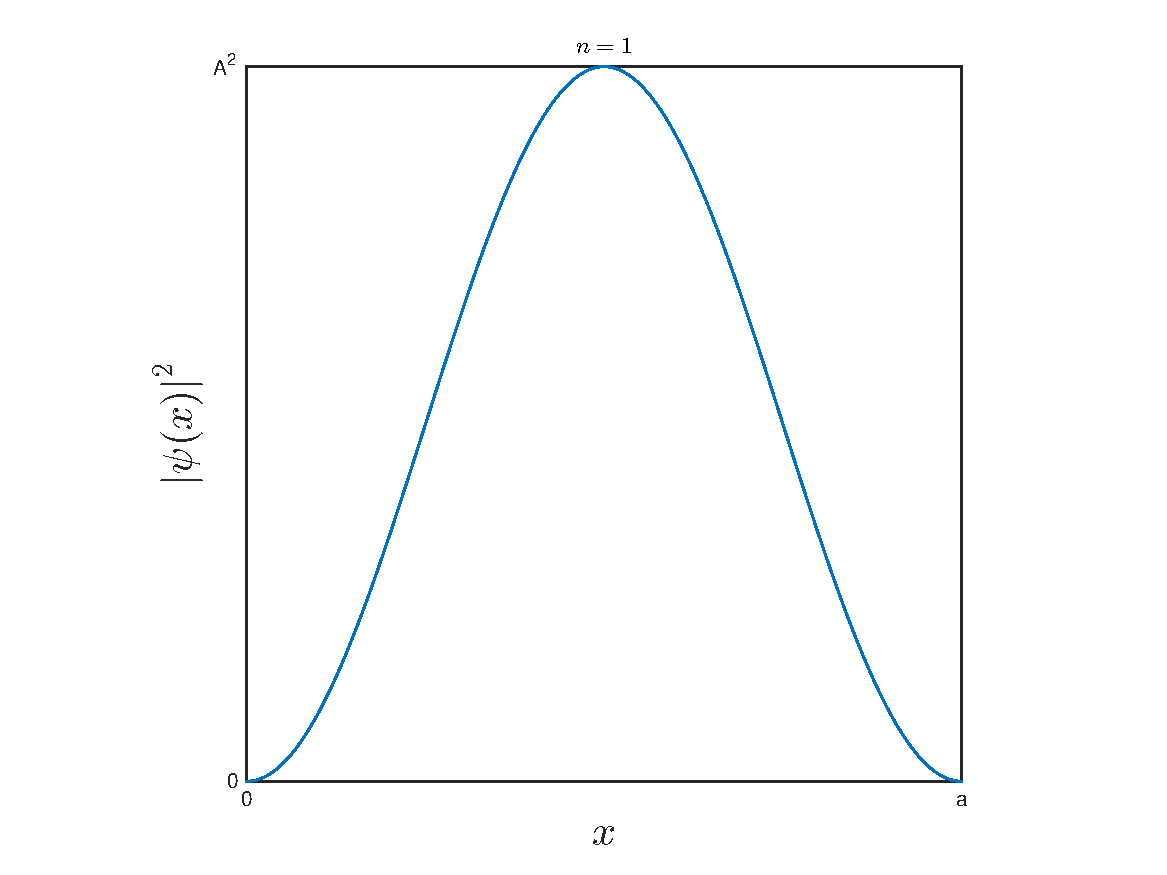
\includegraphics[width = 0.8\textwidth]{fig-probability_distributions_in_infinite_potential_wells_n=1.pdf}
	\caption{Probability distribution of $x$, with $n = 1$, in an infinite square well}
	\label{fig:Probability_distribution_of_$x$,_with_$n_=_1$,_in_an_infinite_square_well}
\end{figure}

\begin{figure}[h]
	\centering
	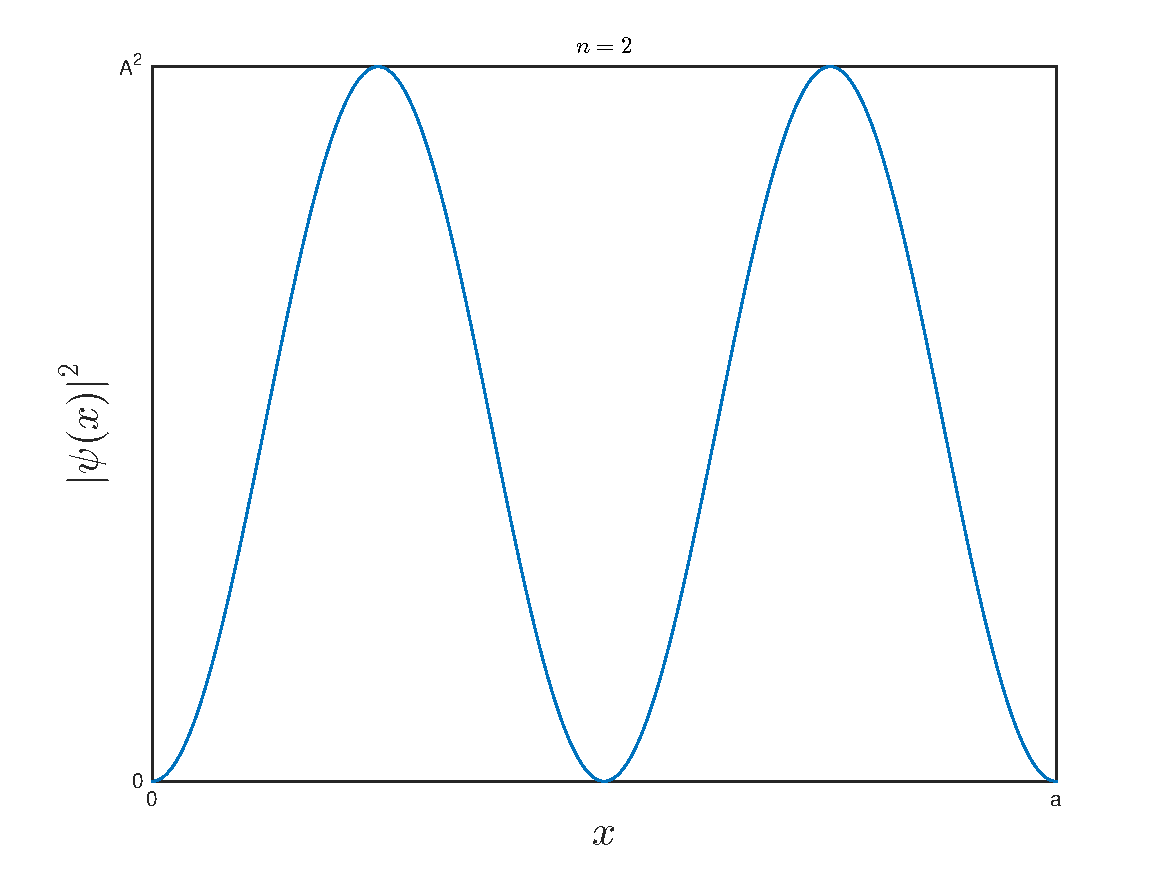
\includegraphics[width = 0.8\textwidth]{fig-probability_distributions_in_infinite_potential_wells_n=2.pdf}
	\caption{Probability distribution of $x$, with $n = 2$, in an infinite square well}
	\label{fig:Probability_distribution_of_$x$,_with_$n_=_2$,_in_an_infinite_square_well}
\end{figure}
Therefore, as these states are stationary
\begin{align*}
	\Psi(x,t) &= \sum\limits_{n = 1}^{\infty} c_n \sqrt{\frac{2}{a}} \sin\left( \frac{n \pi}{a} x \right) e^{-\frac{i E_n t}{\hbar}}
\end{align*}

\begin{question}
	The wave function of a particle of mass $m$ in an infinite square well from $x = 0$ to $x = a$, at time $t = 0$ is given by
	\begin{align*}
		\psi(x,0) &= A x (a - x)
	\end{align*}
	for $0 < x < a$.\\
	\begin{enumerate}
		\item
			Find the general wave function $\psi(x,t)$.
		\item
			What is the probability of measuring the following energies at time $t = 0$?
			\begin{enumerate}
				\item $E_1 = \frac{\pi^2 \hbar^2}{2 m a^2}$
				\item $E_2 = \frac{4 \pi^2 \hbar^2}{2 m a^2}$
				\item $E_3 = \frac{9 \pi^2 \hbar^2}{2 m a^2}$
			\end{enumerate}
	\end{enumerate}
\end{question}

\begin{solution}
	\begin{enumerate}[leftmargin=*]
		\item
			\begin{align*}
				1 &= \int\limits_{0}^{a} A^2 x^2 (a - x)^2 \dif x
			\end{align*}
			Therefore, solving,
			\begin{align*}
				A &= \sqrt{\frac{30}{a^5}}
			\end{align*}
			Therefore,
			\begin{align*}
				A x (a - x) &= \sum\limits_{n = 1}^{\infty} c_n \sqrt{\frac{2}{a}} \sin\left( \frac{n \pi}{a} x \right)
			\end{align*}
			Therefore,
			\begin{align*}
				c_n &= \int\limits_{0}^{a} \sqrt{\frac{2}{a}} \sin\left( \frac{n \pi}{a} x \right) A x (a - x) \dif x\\
				&= \sqrt{\frac{2}{a}} A a \int\limits_{0}^{a} \sin\left( \frac{n \pi}{a} x \right) \dif x - \sqrt{\frac{2}{a}} A \int\limits_{0}^{a} \sin\left( \frac{n \pi}{a} x \right) x^2 \dif x\\
			\end{align*}
			Therefore,
			\begin{align*}
				c_n &=
					\begin{cases}
						0 &;\quad n \text{ is even}\\
						\frac{8 \sqrt{15}}{n^3 \pi^3} &;\quad n \text{ is odd}\\
					\end{cases}
			\end{align*}
			Therefore,
			\begin{align*}
				\psi(x,t) &= \sum\limits_{n = 1,3,5,\dots} \sqrt{\frac{2}{a}} \frac{8 \sqrt{15}}{n^3 \pi^3} \sin\left( \frac{n \pi}{a} x \right) e^{-\frac{i E_n t}{\hbar}}
			\end{align*}
			where
			\begin{align*}
				E_n &= \frac{n^2 \pi^2 \hbar^2}{2 m a^2}
			\end{align*}
		\item
			\begin{enumerate}[leftmargin=*]
				\item
					\begin{align*}
						P(E = E_1) &= |c_1|^2\\
						&= \left( \frac{8 \sqrt{15}}{\pi^3} \right)\\
						&= 0.9986
					\end{align*}
				\item
					\begin{align*}
						P(E = E_2) &= |c_2|^2
						\marginnote
						{
							For even $n$, $c_n$ is zero.
						}\\
						&= 0
					\end{align*}
				\item
					\begin{align*}
						P(E = E_3) &= |c_3|^2\\
						&= \left( \frac{8 \sqrt{15}}{27 \pi^3} \right)\\
						&= 0.0014
					\end{align*}
			\end{enumerate}
	\end{enumerate}
\end{solution}

\begin{question}
	A particle with mass $m$ in an infinite square wall, has initial wave function
	\begin{align*}
		\psi(x,0) &= A \left( \psi_1(x) + \psi_2(x) \right)
	\end{align*}
	\begin{enumerate}
		\item
			Find $A$.
		\item
			Find the general wave function $\psi(x,t)$.
		\item
			What is the probability of measuring the following energies at time $t = 0$?
			\begin{enumerate}
				\item $E_1 = \frac{\pi^2 \hbar^2}{2 m a^2}$
				\item $E_2 = \frac{4 \pi^2 \hbar^2}{2 m a^2}$
			\end{enumerate}
		\item
			Find the wave function if the energy is measured to be $E_1$.
		\item
			Find the expectation value of $x$.
	\end{enumerate}
\end{question}

\begin{solution}
	\begin{enumerate}[leftmargin=*]
		\item
			As the square of the coefficients represents the probability of a particular value,
			\begin{align*}
				1 &= \sum\limits_{n = 1}^{\infty} |c_n|^2\\
				&= 2 A^2\\
				\therefore \frac{1}{\sqrt{2}} &= A
			\end{align*}
		\item
			\begin{align*}
				\psi(x,t) &= A \left( \psi_1(x) e^{-\frac{i E_1 t}{\hbar}} + \psi_2(x) e^{-\frac{i E_2 t}{\hbar}} \right)\\
				&= \frac{1}{\sqrt{2}} \left( \sqrt{\frac{2}{a}} \sin\left( \frac{\pi}{a} x \right) e^{-\frac{i E_1 t}{\hbar}} + \sqrt{\frac{2}{a}} \sin\left( \frac{2 \pi}{a} x \right) e^{-\frac{i E_2 t}{\hbar}} \right)
			\end{align*}
			where
			\begin{align*}
				E_1 &= \frac{\pi^2 \hbar^2}{2 m a^2}\\
				E_2 &= \frac{4 \pi^2 \hbar^2}{2 m a^2}
			\end{align*}
		\item
			\begin{enumerate}[leftmargin=*]
				\item
					\begin{align*}
						P(E = E_1) &= |c_1|^2\\
						&= \left| \frac{1}{\sqrt{2}} e^{-\frac{i E_1 t}{\hbar}} \right|^2\\
						&= \frac{1}{2}
					\end{align*}
				\item
					\begin{align*}
						P(E = E_2) &= |c_2|^2\\
						&= \left| \frac{1}{\sqrt{2}} e^{-\frac{i E_2 t}{\hbar}} \right|^2\\
						&= \frac{1}{2}
					\end{align*}
			\end{enumerate}
		\item
			If $E$ is measured to be $E_1$, then the wave function collapsed to
			\begin{align*}
				\psi(x) &= \psi_1(x) e^{-\frac{i E_1 t}{\hbar}}
			\end{align*}
		\item
			At time $t$,
			\begin{align*}
				\langle x \rangle_t &= \int\limits_{0}^{a} x \left| \psi(x,t) \right|^2 \dif x\\
				&= A^2 \int\limits_{0}^{a} x \left( {\psi_1}^*(x) e^{\frac{i E_1 t}{\hbar}} + {\psi_2}^*(x) e^{\frac{i E_2 t}{\hbar}} \right) \left( \psi_1(x) e^{-\frac{i E_1 t}{\hbar}} + \psi_2(x) e^{-\frac{i E_2 t}{\hbar}} \right) \dif x\\
				&\neq \langle x \rangle_{t = 0}
			\end{align*}
	\end{enumerate}
\end{solution}

%===============================================================================
% Completed upto here
%===============================================================================

\section{Free Particles}

For a free particle,
\begin{align*}
	V(x) &= 0
\end{align*}
Therefore,
\begin{align*}
	\hat{H} \psi(x) &= E \psi(x)\\
	\therefore -\frac{\hbar^2}{2 m} \dod[2]{\psi(x)}{x} &= E \psi(x)\\
	\therefore \dod[2]{\psi(x)}{x} &= -\frac{2 E m \psi(x)}{\hbar^2}\\
	&= -k^2 \psi(x)
\end{align*}
where
\begin{align*}
	k &= \sqrt{\frac{2 m E}{\hbar^2}}
\end{align*}
Therefore,
\begin{align*}
	\psi(x) &= A e^{i k x}
\end{align*}
However, this wave function is not normalizable.
Hence, a free particle cannot exist in a stationary state.\\

The general solution to the time-dependent Schrödinger equation is a linear combination of separable solutions, i.e.
\begin{align*}
	\Psi(x,t) &= \frac{1}{\sqrt{2 \pi}} \int\limits_{-\infty}^{\infty} \varphi(k) e^{i \left( k x - \frac{\hbar k^2}{2 m} t \right)} \dif k
\end{align*}
This function can be normalized, but it carries a multiple $k$s, and hence multiple energies and speeds.

\begin{definition}[Wave packet]
	A solution of the form
	\begin{align*}
		\Psi(x,t) &= \frac{1}{\sqrt{2 \pi}} \int\limits_{-\infty}^{\infty} \varphi(k) e^{i \left( k x - \frac{\hbar k^2}{2 m} t \right)} \dif k
	\end{align*}
	is called a wave packet.
\end{definition}

Therefore, for $t = 0$,
\begin{align*}
	\Psi(x,0) &= \frac{1}{\sqrt{2 \pi}} \int\limits_{-\infty}^{\infty} \varphi(k) e^{i k x} \dif k
\end{align*}
Therefore,
\begin{align*}
	\varphi(k) &= \frac{1}{\sqrt{2 \pi}} \int\limits_{-\infty}^{\infty} \Psi(x,0) e^{-i k x} \dif x
\end{align*}

\begin{question}
	A free particle, initially localized as
	\begin{align*}
		\psi(x,0) &=
			\begin{cases}
				A &;\quad x \in (-a,a)\\
				0 &;\quad x \notin (-a,a)\\
			\end{cases}
	\end{align*}
	where $A$ and $a$ are real and positive.\\
	Find $\psi(x,t)$.
\end{question}

\begin{solution}
	\begin{align*}
		1 &= \int\limits_{-\infty}^{\infty} \left| \psi(x,0) \right|^2 \dif x\\
		&= \int\limits_{-a}^{a} A^2 \dif x\\
		&= 2 a A^2
	\end{align*}
	Therefore,
	\begin{align*}
		A &= \frac{1}{\sqrt{2 a}}
	\end{align*}
	Therefore, taking the inverse Fourier transform,
	\begin{align*}
		\tilde{\psi}(k) &= \frac{1}{\sqrt{2 \pi}} \int\limits_{-\infty}^{\infty} \psi(x,0) e^{-i k x} \dif x\\
		&= \frac{1}{\sqrt{2 \pi}} \frac{1}{\sqrt{2 a}} \int\limits_{-a}^{a} e^{-i k x} \dif x\\
		&= \frac{1}{\sqrt{2 \pi}} \frac{1}{\sqrt{2 a}} \int\limits_{-a}^{a} e^{-i k x} \dif x\\
		&= \frac{1}{\sqrt{4 \pi a}} \left. \frac{1}{-i k} e^{-i k x} \right|_{-a}^{a}\\
		&= \frac{1}{\sqrt{4 \pi a}} \frac{1}{-i k} \left( e^{-i k a} - e^{i k a} \right)\\
		&= \frac{1}{\sqrt{\pi a}} \frac{1}{k} \frac{e^{i k a} - e^{-i k a}}{2 i}\\
		&= \frac{1}{k \sqrt{\pi a}} \sin(k a)
	\end{align*}
	Therefore,
	\begin{align*}
		\psi(x,t) &= \frac{1}{\sqrt{2 \pi}} \int\limits_{-\infty}^{\infty} \tilde{\psi}(k) e^{i k x} e^{-\frac{i E t}{\hbar}} \dif x\\
		&= \frac{1}{\sqrt{2 \pi^2 a}} \int\limits_{-\infty}^{\infty} \frac{\sin(k a)}{k} e^{i k x} e^{-\frac{i k^2 \hbar}{2 m} t} \dif k
	\end{align*}
	If $a$ is very small,
	\begin{align*}
		\tilde{\psi}(k) &= \frac{\sin(k a)}{k \sqrt{\pi a}}\\
		&= \frac{k a}{k \sqrt{\pi a}}\\
		&= \sqrt{\frac{a}{\pi}}
	\end{align*}
	If $a$ is very large,
	\begin{align*}
		\tilde{\psi}(k) &= \frac{\sin(k a)}{k \sqrt{\pi a}}\\
		&= \sqrt{\frac{a}{\pi}} \frac{\sin(k a)}{k a}\\
		&= \sqrt{\frac{a}{\pi}} \sinc(k a)
	\end{align*}
\end{solution}

\section{Finite Potential Wells}

\begin{definition}[Bound state]
	An eigenfunction of $\hat{H}$, which satisfies
	\begin{align*}
		\lim\limits_{x \to \infty} \psi(x) &= 0\\
		\lim\limits_{x \to -\infty} \psi(x) &= 0
	\end{align*}
	is called a bound state.
\end{definition}

\begin{definition}[Scattering state]
	An eigenfunction of $\hat{H}$, which satisfies
	\begin{align*}
		\lim\limits_{x \to \infty} \psi(x) &\neq 0\\
		\lim\limits_{x \to -\infty} \psi(x) &\neq 0
	\end{align*}
	is called a scattering state.
\end{definition}

\begin{theorem}
	A particle in a finite or infinite well is in a bound state.
\end{theorem}

\begin{theorem}
	A free particle is in a scattering state.
\end{theorem}

Consider a finite square well such that
\begin{align*}
	V(x) &=
		\begin{cases}
			-V_0 &;\quad x \in (-a,a)\\
			0 &;\quad x \notin (-a,a)\\
		\end{cases}
\end{align*}
~\\
Consider a particle with energy $-V_0 < E < 0$.\\
For $x < -a$,
\begin{align*}
	V &= 0
\end{align*}
Therefore,
\begin{align*}
	\dod[2]{\psi(x)}{x} &= -\frac{2 m E}{\hbar^2} \psi(x)
\end{align*}
Let
\begin{align*}
	k &= \sqrt{-\frac{2 m E}{\hbar^2}}
\end{align*}
Therefore if $E < 0$, $k$ is real.\\
Therefore,
\begin{align*}
	\dod[2]{\psi(x)}{x} &= k^2 \psi(x)
\end{align*}
Therefore,
\begin{align*}
	\psi(x) &= A e^{k x} + B e^{-k x}
\end{align*}
For the wave function to be normalizable, $\lim\limits_{x \to \infty} \psi(x)$ must be zero.\\
Therefore,
\begin{align*}
	0 &= \lim\limits_{x \to -\infty} \psi(x)\\
	&= \lim\limits_{x \to -\infty} A e^{k x} + B e^{-k x}
\end{align*}
Therefore $B$ must be zero.\\
Therefore,
\begin{align*}
	\psi(x) &= A e^{k x}
\end{align*}
Similarly, for $x > a$,
\begin{align*}
	\psi(x) &= C e^{-k x}
\end{align*}
where
\begin{align*}
	k &= \sqrt{-\frac{2 m E}{\hbar^2}}
\end{align*}
~\\
For $-a < x < a$,
\begin{align*}
	\dod[2]{\psi}{x} &= -\frac{2 m}{\hbar} \left( E - V(x) \right) \psi(x)\\
	&= -\frac{2 m}{\hbar} (E + V_0) \psi(x)
\end{align*}
Let
\begin{align*}
	\beta &= \sqrt{\frac{2 m (E + V_0)}{\hbar^2}}
\end{align*}
Therefore,
\begin{align*}
	\dod[2]{\psi(x)}{x} &= -\beta^2 \psi(x)
\end{align*}
Therefore,
\begin{align*}
	\psi(x) &= D \cos(\beta x) + F \sin(\beta x)
\end{align*}
~\\
Therefore,
\begin{align*}
	\psi(x) &=
		\begin{cases}
			A e^{k x} &;\quad x < -a\\
			D \cos(\beta x) + F \sin(\beta x) &;\quad -a < x < a\\
			C e^{-k x} &;\quad a < x\\
		\end{cases}
\end{align*}
where
\begin{align*}
	k &= \sqrt{-\frac{2 m E}{\hbar^2}}\\
	\beta &= \sqrt{\frac{2 m (E + V_0)}{\hbar^2}}
\end{align*}

\begin{theorem}
	If $V(x)$ is an even function, then the eigenfunctions of $\hat{H}$ are either odd or even.
\end{theorem}

\subsection{Even Wave Functions for Finite Potential Wells}

If $\psi(x)$ is even,
\begin{align*}
	\psi(x) &=
		\begin{cases}
			A e^{k x} &;\quad x < -a\\
			D \cos(\beta x) &;\quad -a < x < a\\
			C e^{-k x} &;\quad a < x\\
		\end{cases}
\end{align*}
As $\left| \psi(x) \right|^2$ represents probability, $\psi(x)$ must always be continuous.\\
As the well is finite, the jump in the expression of $V(x)$ is also finite.
Hence, $\psi'(x)$ must always be continuous.\\
Therefore, as $\psi(x)$ is always continuous,
\begin{align*}
	A e^{-k a} &= D \cos(-\beta a)\\
\end{align*}
Therefore, as $\psi'(x)$ is always continuous,
\begin{align*}
	k A e^{-k a} &= \beta D \cos(\beta a)
\end{align*}
Similarly, for $x = a$,
\begin{align*}
	C e^{-k a} &= D \cos(\beta a)\\
	-k C e^{-k a} &= -\beta D \sin(\beta a)
\end{align*}
Therefore,
\begin{align*}
	A &= C
\end{align*}
Therefore,
\begin{align*}
	k &= \beta \tan(\beta a)
\end{align*}
where
\begin{align*}
	k &= \sqrt{\frac{-2 m E}{\hbar^2}}\\
	\beta &= \sqrt{\frac{2 m (E + V_0)}{\hbar^2}}
\end{align*}
Let
\begin{align*}
	z &= \beta a\\
	y &= k a
\end{align*}
Therefore,
\begin{align*}
	k &= \beta \tan(\beta a)\\
	\therefore k a &= \beta a \tan(\beta a)\\
	\therefore y &= z \tan(z)
\end{align*}
Also,
\begin{align*}
	\beta^2 + k^2 &= \frac{2 m V_0}{\hbar^2}\\
	\therefore z^2 + y^2 &= a^2 \left( \beta^2 + z^2 \right)\\
	&= \frac{2 m V_0 a^2}{\hbar^2}
\end{align*}
Let
\begin{align*}
	{R_0}^2 &= \frac{2 m V_0 a^2}{\hbar^2}
\end{align*}
Therefore,
\begin{align*}
	z^2 + y^2 &= {R_0}^2
\end{align*}
As $a$, $k$, and $B$ are real and positive, $z$ and $y$ also must be real and positive.\\
Therefore,
\begin{figure}[H]
	\centering
	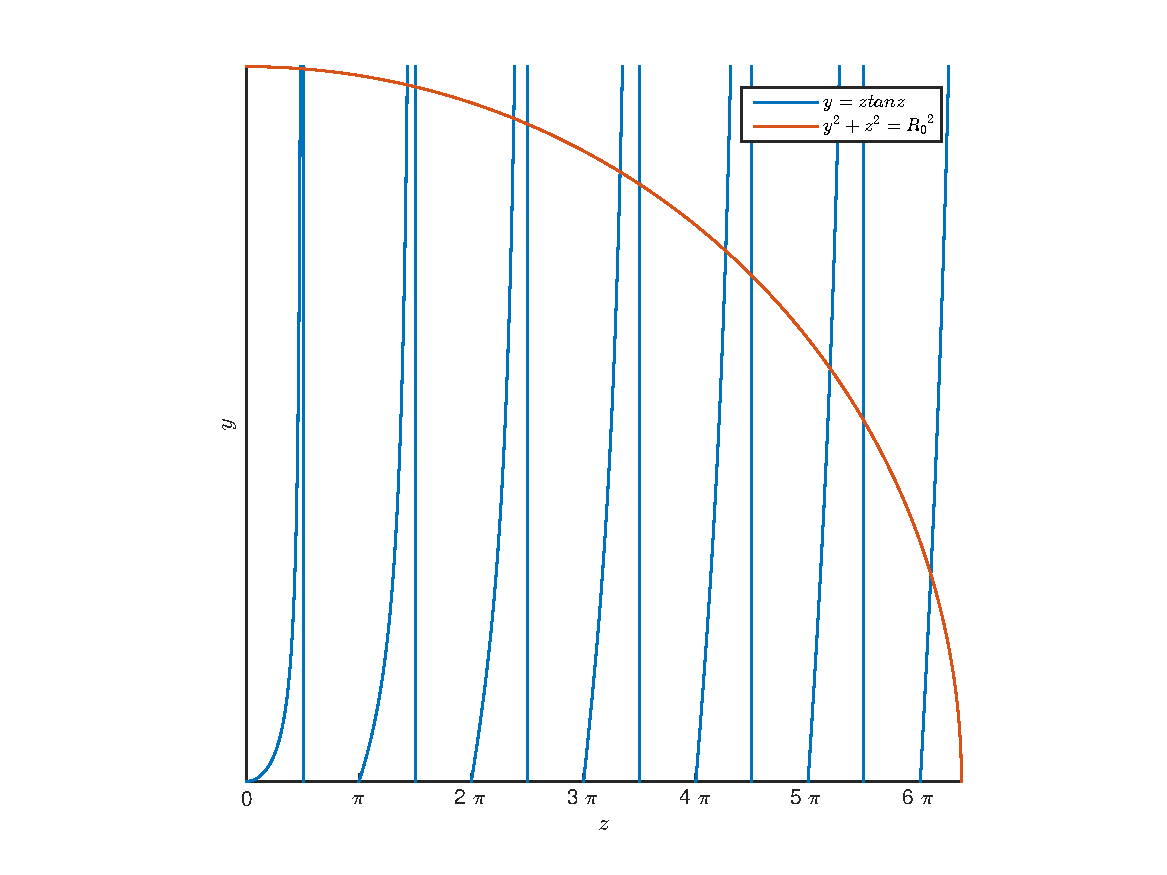
\includegraphics[width = \textwidth]{fig-graphical_solution_for_allowed_energy_levels_for_even_wave_functions_in_finite_potential_well.pdf}
\end{figure}
As the two graphs must intersect at least once, the equation has at least one solution.\\
If $R_0 < \pi$, the graphs intersect exactly once.
Hence, if $R_0 < \pi$, there exists a single solution.\\
If $R_0 \to \infty$, there are infinitely many solutions, $z = \frac{n \pi}{2}$, where $n$ is odd.
Hence,
\begin{align*}
	z_n &= \frac{n \pi}{2}\\
	\therefore \beta_n &= \frac{n \pi}{2 a}
\end{align*}

\begin{question}
	The potential is given by
	\begin{align*}
		V(x) &=
			\begin{cases}
				\infty &;\quad x < 0\\
				0 &;\quad 0 < x < L\\
				V_0 &;\quad L < x\\
			\end{cases}
	\end{align*}
	Solve for the bound states for $E < V_0$.
\end{question}

\begin{solution}
	For $x < 0$,
	\begin{align*}
		\psi(x) &= 0
	\end{align*}
	For $0 < x < L$,
	\begin{align*}
		\psi(x) &= A \sin(k x) + B \cos(k x)
	\end{align*}
	where
	\begin{align*}
		k &= \sqrt{\frac{2 m E}{\hbar^2}}
	\end{align*}
	For $x > L$,
	\begin{align*}
		\psi(x) &= C e^{-\alpha x}
	\end{align*}
	where
	\begin{align*}
		\alpha &= \sqrt{\frac{2 m (V_0 - E)}{\hbar^2}}
	\end{align*}
	For $\psi$ to be continuous at $x = L$, and $\psi$ and $\psi'$ to be continuous at $x = 0$,
	\begin{align*}
		B &= 0\\
		A \sin(k L) &= C e^{-\alpha L}\\
		k A \cos(k L) &= -\alpha C e^{-\alpha L}
	\end{align*}
	Therefore,
	\begin{align*}
		k \cot(k L) &= -\alpha\\
		\therefore k L \cot(k L) &= -\alpha L
	\end{align*}
	Let
	\begin{align*}
		z &= k L\\
		y &= \alpha L
	\end{align*}
	Therefore,
	\begin{align*}
		z \cot(z) &= -y
	\end{align*}
	Also,
	\begin{align*}
		\alpha^2 + k^2 &= \frac{2 m V_0}{\hbar^2}\\
		\therefore \alpha^2 L^2 + k^2 L^2 &= \frac{2 m V_0 L^2}{\hbar^2}\\
		\therefore y^2 + z^2 &= \frac{2 m V_0 L^2}{\hbar^2}
	\end{align*}
\end{solution}

\subsection{Odd Wave Functions for Finite Potential Wells}

If $\psi(x)$ is odd,
\begin{align*}
	\psi(x) &=
		\begin{cases}
			A e^{k x} &;\quad x < -a\\
			F \sin(\beta x) &;\quad -a < x < a\\
			C e^{-k x} &;\quad a < x\\
		\end{cases}
\end{align*}
As $\left| \psi(x) \right|^2$ represents probability, $\psi(x)$ must always be continuous.\\
As the well is finite, the jump in the expression of $V(x)$ is also finite.
Hence, $\psi'(x)$ must always be continuous.\\
Therefore, as $\psi(x)$ is always continuous,
\begin{align*}
	A e^{-k a} &= F \sin(-\beta a)\\
\end{align*}
Therefore, as $\psi'(x)$ is always continuous,
\begin{align*}
	k A e^{-k a} &= \beta F \cos(-\beta a)
\end{align*}
Similarly, for $x = a$,
\begin{align*}
	C e^{-k a} &= F \sin(\beta a)\\
	-k C e^{-k a} &= \beta F \cos(\beta a)
\end{align*}
Therefore,
\begin{align*}
	A &= -C
\end{align*}
Therefore,
\begin{align*}
	-k &= \beta \cot(\beta a)
\end{align*}
where
\begin{align*}
	k &= \sqrt{\frac{-2 m E}{\hbar^2}}\\
	\beta &= \sqrt{\frac{2 m (E + V_0)}{\hbar^2}}
\end{align*}
Let
\begin{align*}
	z &= \beta a\\
	y &= k a
\end{align*}
Therefore,
\begin{align*}
	k &= -\beta \cot(\beta a)\\
	\therefore k a &= -\beta a \cot(\beta a)\\
	\therefore y &= -z \cot(z)
\end{align*}
Also,
\begin{align*}
	\beta^2 + k^2 &= \frac{2 m V_0}{\hbar^2}\\
	\therefore z^2 + y^2 &= a^2 \left( \beta^2 + z^2 \right)\\
	&= \frac{2 m V_0 a^2}{\hbar^2}
\end{align*}
Let
\begin{align*}
	{R_0}^2 &= \frac{2 m V_0 a^2}{\hbar^2}
\end{align*}
Therefore,
\begin{align*}
	z^2 + y^2 &= {R_0}^2
\end{align*}
As $a$, $k$, and $B$ are real and positive, $z$ and $y$ also must be real and positive.\\
Therefore,
\begin{figure}[H]
	\centering
	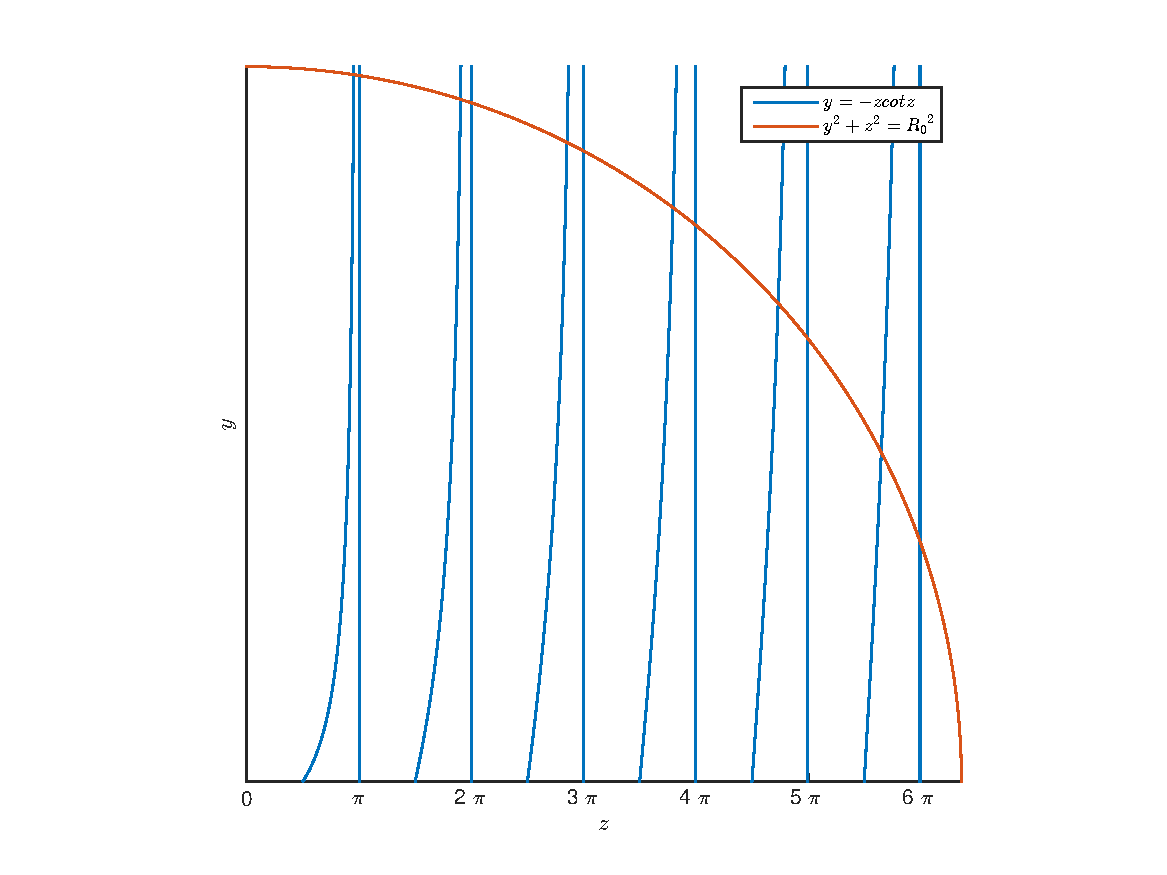
\includegraphics[width = \textwidth]{fig-graphical_solution_for_allowed_energy_levels_for_odd_wave_functions_in_finite_potential_well.pdf}
\end{figure}
If $R_0 < \frac{\pi}{2}$, the two graphs do not intersect.
Therefore, there is no solution.\\
If $R_0 \to \infty$, there are infinitely many solution, $z = n \pi$, where $n$ is positive.
\begin{align*}
	z_n &= n \pi\\
	\therefore \beta_n &= \frac{n \pi}{a}
\end{align*}

\section{$\delta(x)$ Potential}

Consider a potential
\begin{align*}
	V(x) &= -V_0 \delta(x)
\end{align*}
Therefore, for $x < 0$,
\begin{align*}
	\dod[2]{\psi}{x} &= -\frac{2 m}{\hbar^2} \left( E - V(x) \right) \psi\\
	&= -\frac{2 m E}{\hbar^2} \psi
\end{align*}
Let
\begin{align*}
	k &= \sqrt{-\frac{2 m E}{\hbar^2}}
\end{align*}
Therefore, for $E < 0$, $k$ is real.\\
Therefore,
\begin{align*}
	\dod[2]{\psi}{x} &= k^2 \psi
\end{align*}
Therefore,
\begin{align*}
	\psi(x) &= A e^{k x} + B e^{-k x}
\end{align*}
If $x \to \infty$, as the function is normalizable, $\psi = 0$.\\
Therefore,
\begin{align*}
	B &= 0
\end{align*}
Similarly, for $x > 0$,
\begin{align*}
	\psi(x) &= C e^{k x} + D e^{-k x}
\end{align*}
If $x \to -\infty$, as the function is normalizable, $\psi = 0$.\\
Therefore,
\begin{align*}
	C &= 0
\end{align*}
Therefore,
\begin{align*}
	\psi(x) &=
		\begin{cases}
			A e^{k x} &;\quad x < 0\\
			C e^{-k x} &;\quad x > 0\\
		\end{cases}
\end{align*}
Therefore, as $\psi(x)$ represents probability, it is continuous at $x = 0$.\\
Therefore,
\begin{align*}
	A &= C
\end{align*}
Therefore,
\begin{align*}
	\psi(x) &=
		\begin{cases}
			A e^{k x} &;\quad x < 0\\
			A e^{-k x} &;\quad x > 0\\
		\end{cases}
\end{align*}
Therefore,
\begin{align*}
	\psi'(x) &=
		\begin{cases}
			A k e^{k x} &;\quad x < 0\\
			-A k e^{-k x} &;\quad x > 0\\
		\end{cases}
\end{align*}
By the time independent Schrödinger equation,
\begin{align*}
	\psi''(x) &= -\frac{2 m}{\hbar^2} \left( E + V_0 \delta(x) \right) \psi
\end{align*}
Therefore,
\begin{align*}
	\int\limits_{-\varepsilon}^{\varepsilon} \psi''(x) \dif x &= -\frac{2 m}{\hbar^2} \left( E + V_0 \delta(x) \right) \psi(x) \dif x\\
	\therefore \psi'(\varepsilon) - \psi'(-\varepsilon) &= -\frac{2 m}{\hbar^2} \int\limits_{-\varepsilon}^{\varepsilon} E \psi(x) \dif x - \frac{2 m}{\hbar^2} \int\limits_{-\varepsilon}^{\varepsilon} V_0 \delta(x) \psi(x) \dif x\\
	&= -\frac{2 m}{\hbar^2} \left( E \psi(0) \cdot 2 \varepsilon \right) - \frac{2 m}{\hbar^2} V_0 \psi(0)\\
	&= -\frac{2 m}{\hbar^2} V_0 \psi(0)\\
	\therefore -k A - k A &= -\frac{2 m}{\hbar^2} V_0 A\\
	\therefore k &= \frac{m V_0}{\hbar^2}
\end{align*}
Therefore,
\begin{align*}
	k &= \sqrt{-\frac{2 m E}{\hbar^2}}\\
	\therefore E &= -\frac{k^2 \hbar^2}{2 m}\\
	&= -\frac{m {V_0}^2}{2 \hbar^2}
\end{align*}
Normalizing,
\begin{align*}
	A &= \sqrt{k}\\
	&= \sqrt{\frac{m V_0}{\hbar^2}}
\end{align*}

\section{Tunneling}

Consider a potential
\begin{align*}
	V(x) &=
		\begin{cases}
			0 &;\quad x < 0\\
			V_0 &;\quad x > 0\\
		\end{cases}
\end{align*}
Therefore, for $x < 0$,
\begin{align*}
	\dod[2]{\psi(x)}{x} &= -\frac{2 m}{\hbar^2} \left( E - V(x) \right) \psi(x)\\
	&= -\frac{2 m}{\hbar^2} E \psi(x)
\end{align*}
Let
\begin{align*}
	k_1 &= \frac{2 m E}{\hbar^2}
\end{align*}
Therefore,
\begin{align*}
	\psi'' &= -{k_1}^2 \psi
\end{align*}
Therefore, for $x > 0$,
\begin{align*}
	\dod[2]{\psi(x)}{x} &= -\frac{2 m}{\hbar^2} \left( E - V(x) \right) \psi(x)\\
	&= -\frac{2 m}{\hbar^2} (E - V_0) \psi(x)
\end{align*}
Let
\begin{align*}
	k_2 &= -\frac{2 m (E - V_0)}{\hbar^2}
\end{align*}
Therefore,
\begin{align*}
	\psi'' &= {k_2}^2 \psi
\end{align*}
Therefore,
\begin{align*}
	\psi(x) &=
		\begin{cases}
			A e^{i k_1 x} + B e^{-i k_1 x} &;\quad x < 0\\
			C e^{k_2 x} + D e^{-k_2 x} &;\quad x > 0\\
		\end{cases}
\end{align*}
For the function to be normalizable, for $x \to \infty$, $\psi = 0$.\\
Therefore,
\begin{align*}
	C &= 0
\end{align*}
Therefore,
\begin{align*}
	\psi(x) &=
		\begin{cases}
			A e^{i k_1 x} + B e^{-i k_1 x} &;\quad x < 0\\
			D e^{-k_2 x} &;\quad x > 0\\
		\end{cases}
\end{align*}

\subsection{$\delta$ Barrier}

Consider a potential
\begin{align*}
	V(x) &= V_0 \delta(x)
\end{align*}
Consider a single particle approaching the $\delta$ barrier from the left.\\
Therefore, solving the time independent Schrödinger equation,
\begin{align*}
	\psi(x) &=
		\begin{cases}
			A e^{i k x} + B e^{-i k x} &;\quad x < 0\\
			C e^{i k x} + D e^{-i k x} &;\quad 0 < x\\
		\end{cases}
\end{align*}
where
\begin{align*}
	k &= \sqrt{\frac{2 m E}{\hbar^2}}
\end{align*}
Therefore, $A e^{i k x}$ represents the incident wave, $B e^{-i k x}$ represents the reflected wave, and $C e^{i k x}$ represents the transmitted wave.\\
As a single particle approaches the barrier from the left, the wave represented by $D e^{-i k x}$ does not exist.
Hence,
\begin{align*}
	D &= 0
\end{align*}
Therefore,
\begin{align*}
	\psi(x) &=
		\begin{cases}
			A e^{i k x} + B e^{-i k x} &;\quad x < 0\\
			C e^{i k x} &;\quad 0 < x\\
		\end{cases}
\end{align*}
As $\psi(x)$ is continuous at $x = 0$,
\begin{align*}
	A + B &= C
\end{align*}
Therefore, solving,
\begin{align*}
	\psi(x) &=
		\begin{cases}
			i k \left( A e^{i k x} - B e^{-i k x} \right) &;\quad x < 0\\
			i k C e^{i k x} &;\quad 0 < x\\
		\end{cases}
\end{align*}
As the barrier is a Dirac Delta function,
\begin{align*}
	\psi'(\varepsilon) - \psi'(-\varepsilon) &= \frac{2 m v_0}{\hbar^2} \psi(0)
\end{align*}
Therefore,
\begin{align*}
	(i k C) - (i k A - i k B) &= \frac{2 m v_0}{\hbar^2} \psi(0)
\end{align*}
Let
\begin{align*}
	\beta &= \frac{m v_0}{\hbar^2 k}
\end{align*}
Therefore,
\begin{align*}
	\frac{B}{A} &= \frac{-i \beta}{1 + i \beta}\\
	\frac{C}{A} &= \frac{1}{1 + i \beta}
\end{align*}
Similarly, if
\begin{align*}
	V(x) &= -V_0 \delta(x)
\end{align*}
then,
\begin{align*}
	\psi'(\varepsilon) - \psi'(-\varepsilon) &= -\frac{2 m v_0}{\hbar^2} \psi(0)
\end{align*}
Therefore,
\begin{align*}
	(i k C) - (i k A - i k B) &= -\frac{2 m v_0}{\hbar^2} \psi(0)
\end{align*}
Let
\begin{align*}
	\beta &= \frac{m v_0}{\hbar^2 k}
\end{align*}
Therefore,
\begin{align*}
	\frac{B}{A} &= \frac{i \beta}{1 + i \beta}\\
	\frac{C}{A} &= \frac{1}{1 - i \beta}
\end{align*}

\subsection{Double $\delta$ Barrier}

Consider a potential
\begin{align*}
	V(x) &= -\alpha \left( \delta(x + a) + \delta(x - a) \right)
\end{align*}
Therefore,
\begin{align*}
	\psi(x) &=
		\begin{cases}
			A e^{k x} &;\quad x < -a\\
			B e^{k x} + C e^{-k x} &;\quad -a < x < a\\
			D e^{-k x} &;\quad a < x\\
		\end{cases}
\end{align*}
where
\begin{align*}
	k &= \sqrt{-\frac{2 m E}{\hbar^2}}
\end{align*}
Therefore,
\begin{align*}
	\psi(-a + \varepsilon) &= \psi(-a - \varepsilon)\\
	\psi(a + \varepsilon) &= \psi(a - \varepsilon)\\
	\psi'(-a + \varepsilon) - \psi'(-a - \varepsilon) &= -\frac{2 m \alpha}{\hbar^2} \psi(-a)\\
	\psi'(a + \varepsilon) - \psi'(a - \varepsilon) &= -\frac{2 m \alpha}{\hbar^2} \psi(a)
\end{align*}
As $V(x)$ is even, the wave function $\psi(x)$ can be split into odd and even parts, i.e. $\psi_{\text{even}}(x)$ and $\psi_{\text{odd}}(x)$\\
Therefore, for $\psi_{\text{even}}(x)$,
\begin{align*}
	A &= D\\
	B &= C
\end{align*}
Therefore,
\begin{align*}
	\psi_{\text{even}}(x) &=
		\begin{cases}
			A e^{k x} &;\quad x < -a\\
			B \left( e^{k x} + e^{-k x} \right) &;\quad -a < x < a\\
			A e^{-k x} &;\quad a < x\\
		\end{cases}
\end{align*}
Therefore,
\begin{align*}
	\psi'(x) &=
		\begin{cases}
			k A e^{k x} &;\quad x < -a\\
			k B \left( e^{k x} - e^{-k x} \right) &;\quad -a < x < a\\
			-k A e^{-k x} &;\quad a < x\\
		\end{cases}
\end{align*}
Therefore,
\begin{align*}
	\psi(-a + \varepsilon) &= \psi(-a - \varepsilon)\\
	\therefore A e^{-k a} & B \left( e^{-k a} + e^{k a} \right)\\
	\psi'(-a + \varepsilon) - \psi'(-a - \varepsilon) &= -\frac{2 m \alpha}{\hbar^2} \psi(-a)\\
	\therefore k B \left( e^{-k a} - e^{k a} \right) - k A e^{-k a} &= -\frac{2 m \alpha}{\hbar^2} A e^{-k a}
\end{align*}
Therefore, solving,
\begin{align*}
	A &= B \left( e^{2 k a} + 1 \right)\\
	B \left( e^{2 k a} - 1 \right) &= A \left( \frac{2 m \alpha}{\hbar^2 k} - 1 \right)
\end{align*}
Let
\begin{align*}
	z &= 2 k a\\
	c &= \frac{\hbar^2}{2 a m \alpha}
\end{align*}
Therefore,
\begin{align*}
	e^{-2 k a} &= \frac{\hbar^2 k}{m \alpha} - 1\\
	\therefore e^{-z} &= c z - 1
\end{align*}
Therefore, this equation has exactly one solution.
\begin{figure}[H]
	\centering
	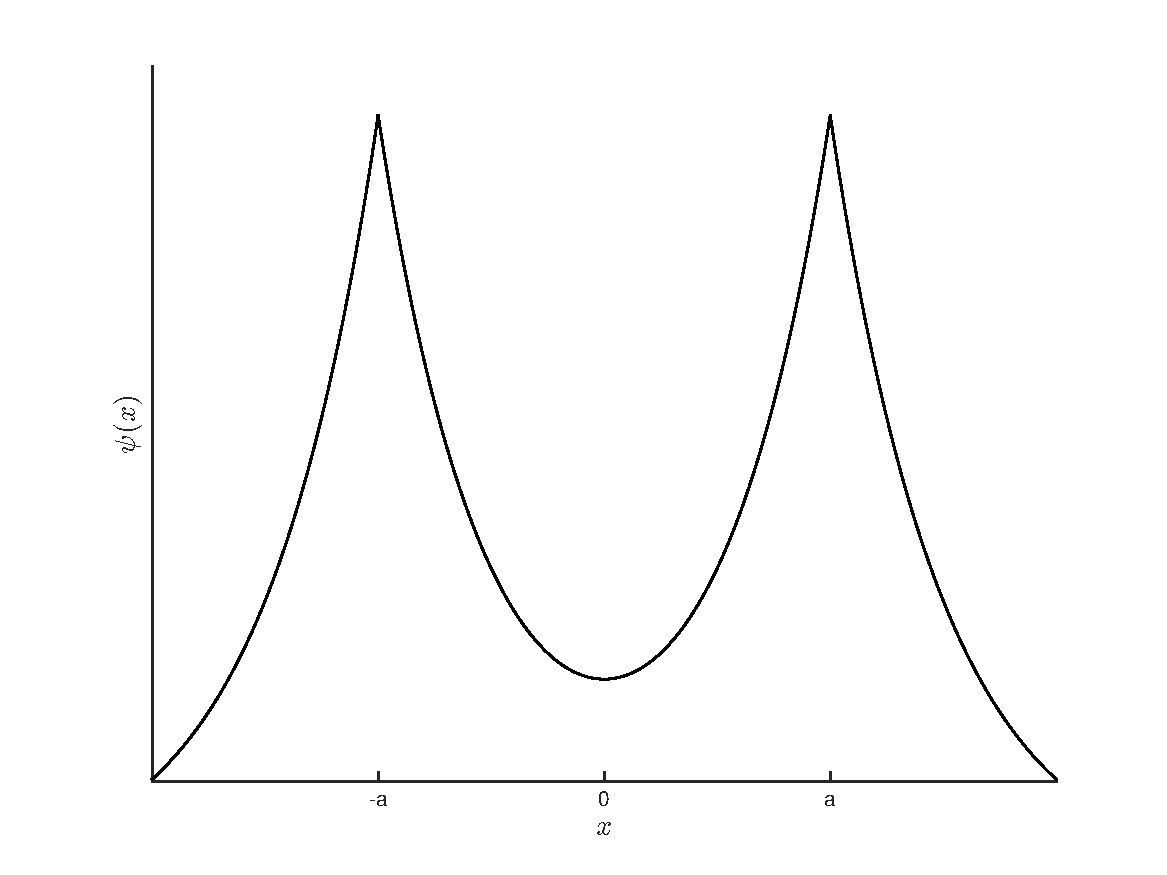
\includegraphics[width = \textwidth]{fig-even_solution_for_double_delta_barrier.pdf}
\end{figure}

Therefore, for $\psi_{\text{odd}}(x)$,
\begin{align*}
	A &= -D\\
	B &= -C
\end{align*}
Therefore,
\begin{align*}
	\psi_{\text{even}}(x) &=
		\begin{cases}
			-A e^{k x} &;\quad x < -a\\
			B \left( e^{k x} - e^{-k x} \right) &;\quad -a < x < a\\
			A e^{-k x} &;\quad a < x\\
		\end{cases}
\end{align*}

\section{Probability Current}

\begin{definition}[Probability current]
	The rate at which the probability distribution passes through the position $x$ is defined to be the probability current.
	It is denoted as
	\begin{align*}
		J(x,t) &= \frac{i \hbar}{2 m} \left( \psi \dpd{\psi^*}{x} - \psi^* \dpd{\psi}{x} \right)
	\end{align*}
\end{definition}

\subsection{$\delta$ Barrier}

Consider a potential
\begin{align*}
	V(x) &= V_0 \delta(x)
\end{align*}
Therefore, the wave function is
\begin{align*}
	\psi(x) &=
		\begin{cases}
			A e^{i k x} + B e^{-i k x} &;\quad x < 0\\
			C e^{i k x} &;\quad x > 0\\
		\end{cases}
\end{align*}
Let the incident, reflected, and transmitted wave functions be
\begin{align*}
	\psi_I &= A e^{i k x}\\
	\psi_R &= B e^{-i k x}\\
	\psi_T &= C e^{i k x}
\end{align*}
Therefore,
\begin{align*}
	\psi_I(x) &= A e^{i k x}\\
	\psi_I(x,t) &= A e^{i k x} e^{-\frac{i E t}{\hbar}}\\
	{\psi_I}^*(x,t) &= A^* e^{-i k x} e^{\frac{i E t}{\hbar}}
\end{align*}
Therefore,
\begin{align*}
	\dpd{\psi_I}{x} &= i k A e^{i k x} e^{-\frac{i E t}{\hbar}}\\
	\dpd{{\psi_I}^*}{x} &= -i k A^* e^{-i k x} e^{\frac{i E t}{\hbar}}
\end{align*}
Therefore, the probability current for the incident wave is
\begin{align*}
	J(x,t) &= \frac{i \hbar}{2 m} \left( \psi \dpd{\psi^*}{x} - \psi^* \dpd{\psi}{x} \right)\\
	J_I(x,t) &= \frac{i \hbar}{2 m} \left( \psi_I \dpd{{\psi_I}^*}{x} - {\psi_I}^* \dpd{\psi_I}{x} \right)\\
	&= \frac{i \hbar}{2 m} \left( -i k |A|^2 - i k |A|^2 \right)\\
	&= \frac{\hbar |A|^2 k}{m}
\end{align*}
Similarly, the probability current for the reflected wave is
\begin{align*}
	J(x,t) &= \frac{i \hbar}{2 m} \left( \psi \dpd{\psi^*}{x} - \psi^* \dpd{\psi}{x} \right)\\
	J_R(x,t) &= \frac{i \hbar}{2 m} \left( \psi_R \dpd{{\psi_R}^*}{x} - {\psi_R}^* \dpd{\psi_R}{x} \right)\\
	&= \frac{i \hbar}{2 m} \left( i k |A|^2 + i k |A|^2 \right)\\
	&= -\frac{\hbar |A|^2 k}{m}
\end{align*}
Similarly, the probability current for the incident wave is
\begin{align*}
	J(x,t) &= \frac{i \hbar}{2 m} \left( \psi \dpd{\psi^*}{x} - \psi^* \dpd{\psi}{x} \right)\\
	J_T(x,t) &= \frac{i \hbar}{2 m} \left( \psi_T \dpd{{\psi_T}^*}{x} - {\psi_T}^* \dpd{\psi_T}{x} \right)\\
	&= \frac{i \hbar}{2 m} \left( -i k |A|^2 - i k |A|^2 \right)\\
	&= \frac{\hbar |A|^2 k}{m}
\end{align*}
Let the transmission and reflection coefficients be $T$ and $R$ respectively.
Therefore, substituting the boundary conditions,
\begin{align*}
	T &= \frac{|J_T|}{|J_I|}\\
	&= \frac{|C|^2}{|A|^2}\\
	&= \frac{1}{1 + \frac{m {V_0}^2}{2 \hbar^2 E}}\\
	R &= \frac{|J_R|}{|J_I|}\\
	&= \frac{|B|^2}{|A|^2}\\
	&= \frac{1}{1 + \frac{2 \hbar^2 E}{m {V_0}^2}}
\end{align*}
Therefore,
\begin{align*}
	T + R &= 1
\end{align*}
This is consistent with the expectations, as the total energy must be conserved.\\
The fact that $T \neq 0$ shows that even though the barrier exists, the particle does not bounce back, but instead tunnels through th barrier.
A classical particle would not exhibit such a behaviour.

\subsection{Finite Barrier}

Consider a potential
\begin{align*}
	V(x) &=
		\begin{cases}
			0 &;\quad x < 0\\
			V_0 &;\quad 0 < x < L\\
			0 &;\quad L < x\\
		\end{cases}
\end{align*}
Therefore, this potential can be considered to be
\begin{align*}
	V(x) &= V_1(x) - V_2(x)
\end{align*}
where
\begin{align*}
	V_1(x) &=
		\begin{cases}
			0 &;\quad x < 0\\
			V_0 &;\quad x > 0\\
		\end{cases}\\
	V_2(x) &=
		\begin{cases}
			0 &;\quad x < L\\
			V_0 &;\quad x > L\\
		\end{cases}
\end{align*}
Consider a single particle approaching the barrier from the left,
Hence, due to tunnelling, a quantum particle can go through this barrier, and the wave function is
\begin{align*}
	\psi(x) &=
		\begin{cases}
			A e^{i k_1 x} + B e^{-i k_1 x} &;\quad x < 0\\
			C e^{k_2 x} + D e^{-k_2 x} &;\quad 0 < x < L\\
			F e^{i k_1 x} + G e^{-i k_1 x} &;\quad L < x\\
		\end{cases}
\end{align*}
where
\begin{align*}
	k_1 &= \sqrt{\frac{2 m E}{\hbar^2}}\\
	k_1 &= \sqrt{-\frac{2 m (E - V_0)}{\hbar^2}}
\end{align*}
Therefore, solving as for the $\delta$ barrier,
\begin{align*}
	T &= \frac{|J_T|}{|J_I|}\\
	&= \frac{|F|^2}{|A|^2}\\
	&= \frac{4 {k_1}^2 {k_2}^2}{\left( {k_1}^2 + {k_2}^2 \right) \sinh^2 (k_2 L) + 4 {k_1}^2 {k_2}^2}\\
	R &= \frac{|J_R|}{|J_I|}\\
	&= \frac{|B|^2}{|A|^2}\\
	&= \frac{\left( {k_1}^2 + {k_2}^2 \right) \sinh^2 (k_2 L)}{\left( {k_1}^2 + {k_2}^2 \right) \sinh^2 (k_2 L) + 4 {k_1}^2 {k_2}^2}
\end{align*}

\section{Quantum Harmonic Oscillator}

Consider a potential
\begin{align*}
	V(x) &= \frac{1}{2} m \omega^2 x^2
\end{align*}
Therefore,
\begin{align*}
	\hat{H} &= \frac{\hat{p}^2}{2 m} + \frac{1}{2} m \omega^2 \hat{x}^2
\end{align*}
and
\begin{align*}
	\hat{H} \psi(x) &= E \psi(x)
\end{align*}
Therefore,
\begin{align*}
	\left( m \omega \hat{x} + i \hat{p} \right) \left( m \omega \hat{x} - i \hat{p} \right) &= \left( m \omega \hat{x} \right)^2 - i m \omega \hat{x} \hat{p} + i m \omega \hat{p} \hat{x} + \hat{p}^2\\
	&= \left( m \omega \hat{x} \right)^2 + i m \omega \left[ \hat{p} , \hat{x} \right] + \hat{p}^2
	\marginnote
	{
		$\left[ \hat{p} , \hat{x} \right]$ is the commutation of $\hat{p}$ and $\hat{x}$.
	}\\
	&= \left( m \omega \hat{x} \right)^2 + i m \omega (- i \hbar) + \hat{p}^2\\
	&= \left( m \omega \hat{x} \right)^2 + m \omega \hbar + \hat{p}^2\\
	\therefore \hat{p}^2 + \left( m \omega \hat{x} \right)^2 &= \left( m \omega \hat{x} + i \hat{p} \right) \left( m \omega \hat{x} - i \hat{p} \right) - m \omega \hbar
\end{align*}
Therefore,
\begin{align*}
	\hat{H} &= \frac{1}{2 m} \left( \hat{p} + m^2 \omega^2 \hat{x}^2 \right)\\
	&= \frac{1}{2 m} \left( \hat{p} + \left( m \omega \hat{x} \right)^2 \right)\\
	&= \frac{1}{2 m} \left( \left( m \omega \hat{x} + i \hat{p} \right) \left( m \omega \hat{x} - i \hat{p} \right) - m \omega \hbar \right)\\
	&= \hbar \omega \left( \frac{1}{\sqrt{2 m \hbar \omega}} \left( m \omega \hat{x} + i \hat{p} \right) \frac{1}{\sqrt{2 m \hbar \omega}} \left( m \omega \hat{x} - i \hat{p} \right) - \frac{1}{2} \right)
\end{align*}

\begin{definition}[Lowering and Raising Operators]
	The raising operator $\hat{a}_+$ and the lowering operator $\hat{a}_-$ are defined as
	\begin{align*}
		\hat{a}_+ &= \frac{1}{\sqrt{2 m \hbar \omega}} \left( m \omega \hat{x} - i \hat{p} \right)\\
		\hat{a}_- &= \frac{1}{\sqrt{2 m \hbar \omega}} \left( m \omega \hat{x} + i \hat{p} \right)
	\end{align*}
\end{definition}

Therefore,
\begin{align*}
	\hat{H} &= \hbar \omega \left( \hat{a}_- \hat{a}_+ - \frac{1}{2} \right)
\end{align*}
The commutation of $\hat{a}_-$ and $\hat{a}_+$ is
\begin{align*}
	\left[ \hat{a}_- , \hat{a}_+ \right] &= \frac{1}{2 m \hbar \omega} \left[ m \omega \hat{x} + i \hat{p} , m \omega \hat{x} - i \hat{p} \right]\\
	&= \frac{1}{2 m \hbar \omega} \left( \left( m \omega \hat{x} + i \hat{p} \right) \left( m \omega \hat{x} - i \hat{p} \right) - \left( m \omega \hat{x} - i \hat{p} \right) \left( m \omega \hat{x} + i \hat{p} \right) \right)\\
	&= \frac{1}{2 m \hbar \omega} \left( \left( m \omega \hat{x} \right)^2 + \hat{p}^2 + m \omega \hbar - \left( m \omega \hat{x} \right)^2 - \hat{p}^2 - \left( i m \omega \hat{x} \hat{p} - i m \omega \hat{p} \hat{x} \right) \right)\\
	&= \frac{1}{2 m \hbar \omega} \left( \left( m \omega \hat{x} \right)^2 + \hat{p}^2 + m \omega \hbar - \left( m \omega \hat{x} \right)^2 - \hat{p}^2 - i m \omega \left[ \hat{x} , \hat{p} \right] \right)\\
	&= \frac{1}{2 m \hbar \omega} \left( \left( m \omega \hat{x} \right)^2 + \hat{p}^2 + m \omega \hbar - \left( m \omega \hat{x} \right)^2 - \hat{p}^2 - i m \omega (i \hbar) \right)\\
	&= \frac{1}{2 m \hbar \omega} \left( \left( m \omega \hat{x} \right)^2 + \hat{p}^2 + m \omega \hbar - \left( m \omega \hat{x} \right)^2 - \hat{p}^2 + m \omega \hbar \right)\\
	&= \frac{1}{2 m \hbar \omega} \left( m \omega \hbar + m \omega \hbar \right)\\
	&= 1
\end{align*}
Therefore,
\begin{align*}
	\left[ \hat{a}_- , \hat{a}_+ \right] &= 1\\
	\left[ \hat{a}_+ , \hat{a}_- \right] &= -1
\end{align*}
The commutation of $\hat{H}$ and $\hat{a}_+$ is
\begin{align*}
	\left[ \hat{H} , \hat{a}_+ \right] &= \left[ \hbar \omega \left( \hat{a}_- \hat{a}_+ - \frac{1}{2} \right) , \hat{a}_+ \right]\\
	&= \hbar \omega \left( \hat{a}_- \hat{a}_+ - \frac{1}{2} \right) a_+ - \hbar \omega a_+ \left( \hat{a}_- \hat{a}_+ - \frac{1}{2} \right)\\
	&= \hbar \omega \left( \hat{a}_- \hat{a}_+ \hat{a}_+ - \frac{1}{2} \hat{a}_+ - \hat{a}_+ \hat{a}_- \hat{a}_+ + \frac{1}{2} \hat{a}_+ \right)\\
	&= \hbar \omega \left[ \hat{a}_- , \hat{a}_+ \right] \hat{a}_+\\
	&= \hbar \omega \hat{a}_+
\end{align*}
Similarly,
\begin{align*}
	\left[ \hat{H} , \hat{a}_- \right] &= -\hbar \omega \hat{a}_-
\end{align*}

\subsection{Effect of $\hat{a}_{\pm}$ on $\psi(x)$}

Let $E$ be an eigenvalue of $\hat{H}$ corresponding to the eigenfunction $\psi(x)$.\\
Therefore,
\begin{align*}
	\hat{H} \psi(x) &= E \psi(x)
\end{align*}
Therefore,
\begin{align*}
	H \hat{a}_+ \psi(x) &= \left( \hbar \omega \hat{a}_+ + \hat{a}_+ \hat{H} \right) \psi(x)\\
	&= \hbar \omega \hat{a}_+ \psi(x) + E \hat{a}_+ \psi(x)\\
	&= (E + \hbar \omega) \hat{a}_+ \psi(x)
\end{align*}
Therefore, $\hat{a}_+ \psi(x)$ is also an eigenfunction of $\hat{H}$ with eigenvalue $(E + \hbar \omega)$.\\
Similarly, $\hat{a}_- \psi(x)$ is also an eigenfunction of $\hat{H}$ with eigenvalue $(E - \hbar \omega)$.\\
~\\
Hence, as the difference between any two consecutive eigenvalues of $H$ is $\hbar \omega$, all eigenvalues are evenly spaced.
Therefore, the energy levels form a ladder as in Figure \ref{fig:Energy_Level_Ladder_for_Quantum_Harmonic_Oscillator}.
Hence, the raising operator can be used in order to go up the ladder, and the lowering operator to go down the ladder.
\begin{figure}[h]
	\centering
	\begin{tikzpicture}
		\def\yMIN{-3};
		\def\yMAX{3};

		\def\l{4};

		\begin{scope}
			\foreach \y in {\yMIN,...,\yMAX}
			{
				\draw (0,\y) -- (\l,\y) node [right] {$E + (\y \hbar \omega)$};
			}
		\end{scope}
	\end{tikzpicture}
	\caption{Energy Level Ladder for Quantum Harmonic Oscillator}
	\label{fig:Energy_Level_Ladder_for_Quantum_Harmonic_Oscillator}
\end{figure}
As the potential $V(x)$ has a minimum value, the ladder is not infinite at its lower end, but is limited from below.\\
~\\
Let the lowest possible eigenfunction be $\psi_0$.
As it is not possible to go lower than this state, the eigenfunction obtained after using the lowering operator on $\psi_0$ must be non-normalizable.
Therefore, as $\psi(x) \equiv 0$ is non-normalizable, let
\begin{align*}
	\hat{a}_- \psi_0 &= 0
\end{align*}
Therefore,
\begin{align*}
	0 &= \frac{1}{\sqrt{2 m \hbar \omega}} \left( m \omega \hat{x} + i \hat{p} \right) \psi_0\\
	&= \left( m \omega \hat{x} + i (-i \hbar) \dpd{}{x} \right) \psi_0\\
	&= \left( m \omega \hat{x} + \hbar \dpd{}{x} \right) \psi_0
\end{align*}
Therefore, solving,
\begin{align*}
	\psi_0(x) &= \left( \frac{m \omega}{\hbar \pi} \right)^{\frac{1}{4}} e^{-\frac{m \omega}{2 \hbar} x^2}
\end{align*}
Therefore, the lowest eigenfunction is a Gaussian function.\\
All other eigenfunctions can be obtained by applying $\hat{a}_+$ repeatedly on $\psi_0$.\\
~\\
Let the eigenvalue of $\hat{H}$ corresponding to $\psi_0$ be $E_0$.
Therefore,
\begin{align*}
	E_0 \psi_0 &= \hat{H} \psi_0\\
	&= \hbar \omega \left( \hat{a}_+ \hat{a}_- + \frac{1}{2} \right) \psi_0\\
	&= \hbar \omega \hat{a}_+ \cancelto{0}{\hat{a}_- \psi_0} + \frac{1}{2} \hbar \omega \psi_0\\
	&= 0 + \frac{1}{2} \hbar \omega \psi_0\\
	&= \frac{1}{2} \hbar \omega \psi_0
\end{align*}
Therefore,
\begin{align*}
	E_0 &= \frac{1}{2} \hbar \omega
\end{align*}
Therefore,
\begin{align*}
	E_n &= \hbar \omega \left( \frac{1}{2} + n \right)
\end{align*}
Let the state obtained after using the raising or lowering operator be
\begin{align*}
	\hat{a}_+ \psi_n &= c_n \psi_{n + 1}\\
	\hat{a}_- \psi_n &= d_n \psi_{n - 1}
\end{align*}
Let
\begin{align*}
	f(x) &= \hat{a}_+ \psi_n\\
	g(x) &= \psi_n
\end{align*}
Therefore, the identity
\begin{align*}
	\int\limits_{-\infty}^{\infty} f^*(x) \left( \hat{a}_{\pm} g(x) \right) \dif x &= \int\limits_{-\infty}^{\infty} \left( \hat{a}_{\mp} f(x) \right)^* g(x) \dif x
\end{align*}
implies
\begin{align*}
	\int\limits_{-\infty}^{\infty} \left( \hat{a}_+ \psi_n \right)^* \left( \hat{a}_+ \psi_n \right) \dif x &= \int\limits_{-\infty}^{\infty} \left( \hat{a}_- \hat{a}_+ \psi_n \right)^* \psi_n \dif x\\
	&= \int\limits_{-\infty}^{\infty} \left( \left( \frac{\hat{H}}{\hbar \omega} + \frac{1}{2} \right) \psi_n \right)^* \psi_n \dif x\\
	&= \int\limits_{-\infty}^{\infty} \left( \left( n + \frac{1}{2} + \frac{1}{2} \right) \psi_n \right)^* \psi_n \dif x\\
	&= \int\limits_{-\infty}^{\infty} \left( (n + 1) \psi_n \right)^* \psi_n \dif x\\
	&= (n + 1) \int\limits_{-\infty}^{\infty} {\psi_n}^* \psi_n \dif x
	\marginnote
	{
		As $\psi_n$ is normalized, $\int\limits_{-\infty}^{\infty} {\psi_n}^* \psi_n \dif x = 1$
	}\\
	&= (n + 1) (1)\\
	\therefore \int\limits_{-\infty}^{\infty} \left( c_n \psi_{n + 1} \right)^* \left( c_n \psi_{n + 1} \right) \dif x &= n + 1\\
	\therefore |c_n|^2 \int\limits_{-\infty}^{\infty} {\psi_{n + 1}}^* \psi_{n + 1} \dif x &= n + 1
\end{align*}
For $\psi_{n + 1}$ to be normalized,
\begin{align*}
	\int\limits_{-\infty}^{\infty} {\psi_{n + 1}}^* \psi_{n + 1} \dif x &= 1
\end{align*}
Therefore,
\begin{align*}
	|c_n|^2 &= n + 1
\end{align*}
Therefore,
\begin{align*}
	c_n &= \sqrt{n + 1}
\end{align*}
Similarly,
\begin{align*}
	d_n &= \sqrt{n}
\end{align*}
Therefore,
\begin{align*}
	\hat{a}_+ \psi_n &= \sqrt{n + 1} \psi_{n + 1}\\
	\hat{a}_- \psi_n &= \sqrt{n} \psi_{n - 1}
\end{align*}
Therefore,
\begin{align*}
	\psi_{n + 1} &= \frac{1}{\sqrt{n + 1}} \hat{a}_+ \psi_n\\
	&= \frac{1}{\sqrt{n - 1}} \hat{a}_+ \left( \frac{1}{\sqrt{n}} \hat{a}_+ \psi_{n - 1} \right)\\
	&= \frac{1}{\sqrt{n - 1}} \frac{1}{\sqrt{n}} \hat{a}_+ \hat{a}_+ \psi_{n - 1}\\
	&= \frac{1}{\sqrt{n}} \frac{1}{\sqrt{n - 1}} \left( \hat{a}_+ \right)^2 \psi_{n - 1}\\
	&\vdots\\
	&= \frac{1}{\sqrt{n!}} \left( \hat{a}_+ \right)^n \psi_0
\end{align*}
Therefore, solving,
\begin{align*}
	\psi_n(x) &= \left( \frac{m \omega}{h \pi} \right)^{\frac{1}{4}} \frac{1}{\sqrt{2^n n!}} e^{-\frac{m \omega x^2}{2 \hbar}} H_n \left( \sqrt{\frac{m \omega}{\hbar} x} \right)
\end{align*}
where $H_i$ are the Hermite polynomials, which are given by
\begin{align*}
	H_n(x) &= (-1)^n e^{x^2} \dod[n]{}{x} e^{-x^2}
\end{align*}
Therefore,
\begin{align*}
	H_0 &= 1\\
	H_1 &= 2 x\\
	H_2 &= 4 x^2 - 2\\
	H_3 &= 8 x^3 - 12 x\\
	H_4 &= 16 x^4 - 48 x^2 + 12\\
	&\vdots
\end{align*}

\subsection{Potential Energy}

Let the potential energy for the harmonic oscillator be $V$.\\
Therefore, the expectation value of $V$ for the $n$th state of the harmonic oscillator is
\begin{align*}
	\langle V \rangle &= \left\langle \frac{1}{2} m \omega^2 \hat{x}^2 \right\rangle\\
	&= \frac{1}{2} m \omega^2 \int\limits_{-\infty}^{\infty} {\psi_n}^* \hat{x}^2 \psi_n \dif x
\end{align*}
Also,
\begin{align*}
	\hat{x} &= \sqrt{\frac{\hbar}{2 m \omega}} \left( \hat{a}_+ + \hat{a}_- \right)
\end{align*}
Therefore, substituting and solving,
\begin{align*}
	\langle V \rangle &= \frac{\hbar \omega}{2} \left( n + \frac{1}{2} \right)\\
	&= \frac{E_n}{2}
\end{align*}

\begin{question}
	Consider a quantum harmonic oscillator with
	\begin{align*}
		V(x) &= \frac{1}{2} m \omega^2 x^2
	\end{align*}
	Assume
	\begin{align*}
		\psi(x,0) &= \frac{1}{\sqrt{2}} \left( \psi_0(x) + i \psi_1(x) \right)
	\end{align*}
	\begin{enumerate}
		\item
			At $t = 0$, what is the probability of measuring the energy to be $\frac{3}{2} \hbar \omega$?
		\item
			At $t = 0$, what is the probability of measuring the energy to be $\frac{11}{2} \hbar \omega$?
		\item
			At $t = 0$, the energy is measured and found to be the maximum possible value.
			What is the state of the system after measurement?
	\end{enumerate}
\end{question}

\begin{solution}
	\begin{enumerate}[leftmargin=*]
		\item
			\begin{align*}
				E_n &= \hbar \omega \left( n + \frac{1}{2} \right)
			\end{align*}
			Therefore, if
			\begin{align*}
				E &= \frac{3}{2} \hbar \omega
			\end{align*}
			then $n = 1$.\\
			Therefore, the probability of measuring the given energy is the probability of $n$ being $1$.\\
			Therefore,
			\begin{align*}
				P\left( E = \frac{3}{2} \hbar \omega \right) &= |c_2|^2\\
				&= \left| \frac{i}{\sqrt{2}} \right|^2\\
				&= \frac{1}{2}
			\end{align*}
		\item
			\begin{align*}
				E_n &= \hbar \omega \left( n + \frac{1}{2} \right)
			\end{align*}
			Therefore, if
			\begin{align*}
				E &= \frac{11}{2} \hbar \omega
			\end{align*}
			then $n = 5$.\\
			As the wave function at $t = 0$ is a combination of $\psi_0$ and $\psi_1$ only, the probability of $n$ being $5$, and hence the probability of measuring the given energy is $0$.
		\item
			As the energy is measured to be the maximum possible, i.e. $E_1$, the wave function collapses to $\psi_1(x)$.
	\end{enumerate}
\end{solution}

\begin{question}
	Consider a quantum particle of mass $m$ in the potential
	\begin{align*}
		V(x) &=
			\begin{cases}
				\infty &;\quad x < 0\\
				\frac{1}{2} m \omega^2 x^2 &;\quad x > 0\\
			\end{cases}
	\end{align*}
	Find the allowed energies of the particles.
\end{question}

\begin{solution}
	If $x < 0$, $V(x) = \infty$.\\
	Therefore,
	\begin{align*}
		\psi(x) &= 0
	\end{align*}
	If $x > 0$, the wave function is that for a quantum harmonic oscillator.\\
	Therefore,
	\begin{align*}
		\psi(x) &= \left( \frac{m \omega}{\hbar \pi} \right)^{\frac{1}{4}} \frac{1}{\sqrt{2^n n!}} e^{-\frac{m \omega x^2}{2 \hbar}} H_n \left( \sqrt{\frac{m \omega}{\hbar}} x \right)
	\end{align*}
	Therefore,
	\begin{align*}
		\psi(x) &=
			\begin{cases}
				0 :\quad x < 0\\
				\left( \frac{m \omega}{\hbar \pi} \right)^{\frac{1}{4}} \frac{1}{\sqrt{2^n n!}} e^{-\frac{m \omega x^2}{2 \hbar}} H_n \left( \sqrt{\frac{m \omega}{\hbar}} x \right) &;\quad x > 0\\
			\end{cases}
	\end{align*}
	For $\psi$ to be continuous,
	\begin{align*}
		\psi(0) &= 0
	\end{align*}
	Therefore, solving, the boundary conditions are satisfied by odd $n$ only.\\
	Therefore,
	\begin{align*}
		E_n &= \hbar w \left( n + \frac{1}{2} \right)
	\end{align*}
	Therefore, the spacing between the energy levels is $2 \hbar \omega$
\end{solution}

\section{3D Harmonic Oscillator}

\begin{table}[h]
	\centering
	\begin{tabular}{l l l}
		\toprule
		1D Schrödinger Equation & 3D Schrödinger Equation\\
		\midrule
		$\displaystyle \psi(x,t)$ & $\displaystyle \psi(x,y,z,t)$\\
		$\displaystyle \int\limits_{-\infty}^{\infty} |\psi|^2 \dif x = 1$ & $\displaystyle \iiint\limits_{-\infty}^{\infty} |\psi|^2 \dif x \dif y \dif z = 1$\\
		$\displaystyle \hat{H} = \frac{{\hat{p}_x}^2}{2 m} + V(x)$ & $\displaystyle \hat{H} = \frac{{\hat{p}_x}^2 + {\hat{p}_y}^2 + {\hat{p}_z}^2}{2 m} + V(x,y,z)$\\
		$\displaystyle \hat{H} = -\frac{i \hbar}{m} \left( \dpd[2]{}{x} + \dpd[2]{}{y} + \dpd[2]{}{z} \right) + V(x,y,z)$ & $\displaystyle \hat{H} = -\frac{i \hbar}{m} \left( \dpd[2]{}{x} \right) + V(x,y,z)$\\
		$\Psi(x,t) = \psi(x) \varphi(t)$ & $\Psi(x,y,z,t) = \psi(x,y,z) \varphi(t)$\\
		$\varphi(t) = e^{-\frac{i E t}{\hbar}}$ & $\varphi(t) = e^{-\frac{i E t}{\hbar}}$\\
		$\Psi(x,t) = \sum c_n \psi_n(x) e^{-\frac{i E t}{\hbar}}$ & $\Psi(x,y,z,t) = \sum c_n \psi_n(x,y,z) e^{-\frac{i E t}{\hbar}}$\\
		\bottomrule
	\end{tabular}
	\caption{Comparison of 1D and 3D Schrödinger Equations}
	\label{tab:Comparison_of_1D_and_3D_Schrodinger_Equations}
\end{table}

The Hamiltonian operator in 3D is
\begin{align*}
	\hat{H} &= -\frac{\hbar^2}{2 m} \left( \dpd[2]{}{x} + \dpd[2]{}{y} + \dpd[2]{}{z} \right) + \frac{1}{2} m \omega^2 \left( x^2 + y^2 + z^2 \right)
\end{align*}
Let $E$ be the eigenvalue of $\hat{H}$ corresponding to $\psi(x,y,z)$.\\
Therefore,
\begin{align*}
	\hat{H} \psi(x,y,z) &= E \psi(x,y,z)
\end{align*}
Separating the variables, let
\begin{align*}
	\psi(x,y,z) &= \psi_x(x) \psi_y(y) \psi_z(z)
\end{align*}
Therefore,
\begin{align*}
	\left( -\frac{\hbar}{2 m} \dpd[2]{}{x} + \frac{1}{2} m \omega^2 x^2 \right) \psi_x(x) &= E_n \psi_x(x)\\
	\left( -\frac{\hbar}{2 m} \dpd[2]{}{y} + \frac{1}{2} m \omega^2 y^2 \right) \psi_y(y) &= E_m \psi_y(y)\\
	\left( -\frac{\hbar}{2 m} \dpd[2]{}{z} + \frac{1}{2} m \omega^2 z^2 \right) \psi_z(z) &= E_l \psi_z(z)
\end{align*}
Therefore,
\begin{align*}
	E &= E_n + E_m + E_l\\
	&= \frac{3}{2} \hbar \omega + \hbar \omega (n + m + l)
\end{align*}

\begin{question}
	Consider a single particle in a 3D infinite well of side $a$, which is equivalent to a single particle in a box of side $a$, cornered at $(0,0,0)$.
	The potential is given by
	\begin{align*}
		V(x,y,z) &=
			\begin{cases}
				0 &;\quad \text{inside the box}\\
				\infty &;\quad \text{outside the box}\\
			\end{cases}
	\end{align*}
	Find the wave function of the particle.
\end{question}

\begin{solution}
	As the potential outside the box is infinite, for any point outside the box,
	\begin{align*}
		\psi(x) &= 0
	\end{align*}
	For a point inside the box,
	\begin{align*}
		\hat{H} &= -\frac{\hbar^2}{2 m} \left( \dpd[2]{}{x} + \dpd[2]{}{y} + \dpd[2]{}{z} \right)
	\end{align*}
	Let $E$ be the eigenvalue of $\hat{H}$ corresponding to $\psi(x,y,z)$.
	Therefore,
	\begin{align*}
		\hat{H} \psi(x,y,z) &= E \psi(x,y,z)
	\end{align*}
	Therefore, separating the variables,
	\begin{align*}
		\psi(x,y,z) &= \psi_x(x) \psi_y(y) \psi_z(z)
	\end{align*}
	Therefore,
	\begin{align*}
		\hat{H} \psi(x,y,z) &= E \psi(x,y,z)\\
		\therefore \hat{H} \left( \psi_x(x) \psi_y(y) \psi_z(z) \right) &= E \psi_x(x) \psi_y(y) \psi_z(z)\\
		\therefore -\frac{\hbar^2}{2 m} \left( {\psi_x}'' \psi_y \psi_z + \psi_x {\psi_y}'' \psi_z + \psi_x \psi_y {\psi_z}'' \right) &= E \psi_x \psi_y \psi_z\\
		\therefore \frac{{\psi_x}''}{\psi_x} + \frac{{\psi_y}''}{\psi_y} + \frac{{\psi_z}''}{\psi_z} &= -\frac{2 m E}{\hbar^2}
	\end{align*}
	Let
	\begin{align*}
		k_x &= \sqrt{-\frac{{\psi_x}''}{\psi_x}}\\
		k_y &= \sqrt{-\frac{{\psi_y}''}{\psi_y}}\\
		k_z &= \sqrt{-\frac{{\psi_z}''}{\psi_z}}\\
		k &= \sqrt{\frac{2 m E}{\hbar^2}}
	\end{align*}
	Therefore,
	\begin{align*}
		{k_x}^2 + {k_y}^2 + {k_z}^2 &= k^2
	\end{align*}
	Therefore,
	\begin{align*}
		\psi_x(x) &= A \sin(k_x x) + B \cos(k_x x)\\
		\psi_y(y) &= C \sin(k_y y) + D \cos(k_y y)\\
		\psi_z(z) &= F \sin(k_z z) + G \cos(k_z z)
	\end{align*}
	Therefore, as $\psi$ is continuous at $(0,0,0)$, solving,
	\begin{align*}
		B &= 0\\
		D &= 0\\
		G &= 0\\
		k_x a &= n_x \pi\\
		k_y a &= n_y \pi\\
		k_z a &= n_z \pi\\
	\end{align*}
	Therefore,
	\begin{align*}
		\psi_x(x) &= A \sin(k_x x)\\
		\psi_y(y) &= C \sin(k_y y)\\
		\psi_z(z) &= F \sin(k_z z)
	\end{align*}
	Therefore,
	\begin{align*}
		\psi(x,y,z) &= N \sin\left( \frac{n_x \pi}{a} x \right) + \sin\left( \frac{n_y \pi}{a} y \right) + \sin\left( \frac{n_z \pi}{a} z \right)
	\end{align*}
	Therefore, normalizing,
	\begin{align*}
		\int\limits_{-\infty}^{\infty} |\psi|^2 \dif x \dif y \dif z &= 1
	\end{align*}
	Therefore, solving,
	\begin{align*}
		N &= \left( \sqrt{\frac{2}{a}} \right)^3
	\end{align*}
	Therefore,
	\begin{align*}
		E &= \frac{k^2 \hbar^2}{2 m}\\
		&= \frac{\left( {k_x}^2 + {k_y}^2 + {k_z}^2 \right) \hbar^2}{2 m}\\
		&= \frac{\left( \left( \frac{n_x \pi}{a} \right)^2 + \left( \frac{n_y \pi}{a} \right)^2 + \left( \frac{n_z \pi}{a} \right)^2 \right) \hbar^2}{2 m}
	\end{align*}
	Therefore, there is degeneracy in the energies, i.e., for different combinations of $n_x$, $n_y$, $n_z$, there exist different wave functions with same energy.
\end{solution}


\section{Angular Momentum}

\begin{definition}[Angular momentum operators]
	The angular momentum operators in the $x$, $y$, $z$ directions are defined as
	\begin{align*}
		\hat{L}_x &= \hat{y} \hat{p}_z - \hat{z} \hat{p}_y\\
		\hat{L}_y &= \hat{z} \hat{p}_x - \hat{x} \hat{p}_z\\
		\hat{L}_z &= \hat{x} \hat{p}_y - \hat{y} \hat{p}_x
	\end{align*}
	where $\hat{x}$, $\hat{y}$, $\hat{z}$ are the position operators in the $x$, $y$, $z$ directions respectively, and $\hat{p}_x$, $\hat{p}_y$, $\hat{p}_z$ are the momentum operators in the $x$, $y$, $z$ directions respectively.
\end{definition}

\section{Commutation Relations for 3D Operators}

\begin{theorem}
	\begin{align*}
		\left[ \hat{i},\hat{j} \right] &= i \hbar \delta_{i j}\\
		\left[ \hat{p}_i,\hat{p}_j \right] &= 0\\
		\left[ \hat{i},\hat{p}_i \right] &= 0
	\end{align*}
	where $i$, $j$ can be $x$, $y$, $z$.
\end{theorem}

\subsection{Angular Momentum Operators in Orthogonal Directions}

\begin{align*}
	\left[ \hat{L}_x,\hat{L}_y \right] &= \left( \hat{y} \hat{p}_z - \hat{z} \hat{p}_y \right) \left( \hat{z} \hat{p}_x - \hat{x} \hat{p}_x \right) - \left( \hat{z} \hat{p}_x - \hat{x} \hat{p}_z \right) \left( \hat{y} \hat{p}_z - \hat{z} \hat{p}_y \right)\\
	&= \quad \underbrace{\hat{y} \hat{p}_z \hat{z} \hat{p}_x}_{1} - \underbrace{\hat{y} \hat{p}_z \hat{x} \hat{p}_z}_{2} - \underbrace{\hat{z} \hat{p}_y \hat{z} \hat{p}_x}_{3} + \underbrace{\hat{z} \hat{p}_y \hat{x} \hat{p}_z}_{4}\\
	&\quad - \underbrace{\hat{z} \hat{p}_x \hat{y} \hat{p}_z}_{5} + \underbrace{\hat{z} \hat{p}_x \hat{z} \hat{p}_y}_{6} + \underbrace{\hat{x} \hat{p}_z \hat{y} \hat{p}_z}_{7} - \underbrace{\hat{x} \hat{p}_z \hat{z} \hat{p}_y}_{8}
\end{align*}
Therefore, term $2$ is
\begin{align*}
	\hat{y} \hat{p}_z \hat{x} \hat{p}_z &= \hat{y} \hat{x} \hat{p}_z \hat{p}_z
	\marginnote
	{
		$\left[ \hat{x},\hat{p}_z \right] = 0$
	}\\
	&= x y p_z p_x
	\marginnote
	{
		$\left[ \hat{y},\hat{x} \right] = 0$
	}\\
	&= x p_z y p_z
	\marginnote
	{
		$\left[ \hat{y},\hat{p}_z \right] = 0$
	}
\end{align*}
Therefore, term $2$ is equal to term $7$.\\
similarly, solving,
\begin{align*}
	\left[ \hat{L}_x,\hat{L}_y \right] &= i \hbar \hat{L}_z\\
	\left[ \hat{L}_y,\hat{L}_z \right] &= i \hbar \hat{L}_x\\
	\left[ \hat{L}_z,\hat{L}_x \right] &= i \hbar \hat{L}_y
\end{align*}

\subsection{Angular Momentum Operators and Square of Angular Momentum Operator}

\begin{align*}
	\left[ \hat{L}^2, \hat{L}_x \right] &= \left[ {\hat{L}_x}^2 + {\hat{L}_y}^2 + {\hat{L}_z}^2 , \hat{L}_x \right]\\
	&= {\hat{L}_x}^3 + \hat{L}_y \hat{L}_y \hat{L}_x + \hat{L}_z \hat{L}_z \hat{L}_x - {\hat{L}_x}^3 - \hat{L}_x \hat{L}_y \hat{L}_y - \hat{L}_x \hat{L}_z \hat{L}_z
\end{align*}
Therefore,
\begin{align*}
	\hat{L}_y \hat{L}_y \hat{L}_x &= -i \hbar \hat{L}_y \hat{L}_z + \hat{L}_y \hat{L}_x \hat{L}_y
	\marginnote
	{
		$\hat{L}_y \hat{L}_x = \left[ \hat{L}_y,\hat{L}_x \right] + \hat{L}_x \hat{L}_y = -i \hbar \hat{L}_z + \hat{L}_x \hat{L}_y$
	}\\
	&= -i \hbar \hat{L}_y \hat{L}_z - i \hbar \hat{L}_z \hat{L}_y + \hat{L}_x \hat{L}_y \hat{L}_y
\end{align*}
Similarly,
\begin{align*}
	\hat{L}_z \hat{L}_z \hat{L}_x &= i \hbar \hat{L}_z \hat{L}_y + i \hbar \hat{L}_y \hat{L}_z + \hat{L}_x \hat{L}_z \hat{L}_z
\end{align*}
Therefore, substituting and solving,
\begin{align*}
	\left[ \hat{L}^2,\hat{L}_x \right] &= 0
\end{align*}
Similarly,
\begin{align*}
	\left[ \hat{L}^2,\hat{L}_y \right] &= 0\\
	\left[ \hat{L}^2,\hat{L}_z \right] &= 0
\end{align*}
Therefore, as the commutation relations are zeros, the operators have common eigenfunctions.\\
Let $Y_{l m}$ be an eigenfunction of the momentum operator $\hat{L}_z$.\\
Therefore,
\begin{align*}
	\hat{L}_z Y_{l m} &= m \hbar Y_{l m}\\
	\hat{L}^2 Y_{l m} &= l (l + 1) \hbar^2 Y_{l m}
\end{align*}
where $m$ and $l$ are real constants.\\
Let
\begin{align*}
	\hat{L}_+ &= \hat{L}_x + i \hat{L}_y\\
	\hat{L}_- &= \hat{L}_x - i \hat{L}_y
\end{align*}
be two operators.\\
Therefore, the commutation relations on $\hat{L}_+$ and $\hat{L}_-$ are
\begin{align*}
	\left[ \hat{L}_z,\hat{L}_- \right] &= \hbar \hat{L}_+\\
	\left[ \hat{L}_z,\hat{L}_- \right] &= -\hbar \hat{L}_-\\
	\left[ \hat{L}^2,\hat{L}_+ \right] &= 0\\
	\left[ \hat{L}^2,\hat{L}_- \right] &= 0
\end{align*}

\subsection{Effect of $\hat{L}_{\pm}$ on $Y_{l m}$}

\begin{align*}
	\hat{L}_z \hat{L}_+ Y_{l m} &= \left( \hbar \hat{L}_+ + \hat{L}_+ \hat{L}_z \right) Y_{l m}
	\marginnote
	{
		$\hat{L}_z \hat{L}_+ = \left[ \hat{L}_z,\hat{L}_+ \right] + \hat{L}_+ \hat{L}_z = \hbar \hat{L}_+ + \hat{L}_+ \hat{L}_z$
	}\\
	&= \hbar (m + 1) \hat{L}_+ Y_{l m}
	\marginnote
	{
		$\hat{L}_z Y_{l m} = m \hbar + Y_{l m}$
	}
\end{align*}
Therefore, $\hat{L}_+ Y_{l m}$ is also an eigenfunction of $\hat{L}_z$, with eigenvalue $\hbar (m + 1)$.\\
Similarly,
\begin{align*}
	\hat{L}^2 \hat{L}_+ Y_{l m} &= \hat{L}_+ \hat{L}^2 Y_{l m}\\
	&= \hbar^2 l (l + 1) \hat{L}_+ Y_{l m}
\end{align*}
Therefore, $\hat{L}_+ Y_{l m}$ is also an eigenfunction of $\hat{L}^2$, but with the same eigenvalue, $\hbar^2 l (l + 1)$.

\newpage
\part{Solid State Physics}

\section{Lecturer Information}

\textbf{Tammy Ben-Yaacov}\\
~\\
E-mail: \href{mailto:tammybenyaacov@gmail.com}{tammybenyaacov@gmail.com}\\

\section{Required Reading}

\begin{enumerate}
	\item Streetman, B. Solid State Electronic Devices
\end{enumerate}

\section{Additional Reading}

\begin{enumerate}
	\item Kittel, Introduction to solid state physics, John Wiley \& Sons.
	\item Pierret. Advanced semiconductor Fundamentals, Prentice Hall.
	\item Ashcroft, Solid State Physics, Harcourt college publishers.
\end{enumerate}

\newpage
\section{Electrons}

\begin{definition}[Particle nature of electrons]
	An electron behaves as a negatively charged charge carrying particle.\\
	The magnitude of the charge on it is
	\begin{align*}
		q & = 1.602 \times 10^{-19} \coulomb
	\end{align*}
	Its mass is
	\begin{align*}
		m_0 & = 9.11 \times 10^{-31} \kilogram
	\end{align*}
\end{definition}

\begin{definition}[Wave nature of electrons]
	Electrons exhibit wave-like properties, in addition to particle-like properties.\\
	The energy transmitted by a wave is
	\begin{align*}
		E & = h \nu \\
                  & = \frac{h c}{\lambda}
	\end{align*}
	where
	\begin{align*}
		h       & = \text{Planck's constant} \left( 6.626 \times 10^{-34} \right) \\
		\nu     & = \text{frequency}                                              \\
		c       & = \text{speed of light}                                         \\
		\lambda & = \text{wavelength}
	\end{align*}
\end{definition}

\section{Semiconductors}

\begin{law}[Ohm's Law]
	The voltage across two points on a conductor is directly proportional to the current through the conductor.
	The constant of proportionality is called the resistance of the conductor.
	\begin{equation*}
		\frac{V}{I} = R
	\end{equation*}
	\label{Ohm's_Law}
\end{law}

\begin{law}[Microscopic Ohm's Law]
	\begin{equation*}
		\overrightarrow{J}  = \sigma \overrightarrow{E}
	\end{equation*}
	where $\overrightarrow{J}$ is the current density, $\sigma$ is the conductivity, $\overrightarrow{E}$ is the electric field in the resistor.
	\label{Microscopic_Ohm's_Law}
\end{law}

\begin{definition}[Resistivity]
	If
	\begin{equation*}
		R = \rho \frac{L}{A}
	\end{equation*}
	where $R$ is the resistance of the resistor, $L$ is the length of the resistor, and $A$ is the cross-sectional area of the resistor, then $\rho$ is called the resistivity of the resistor.\\
	$\sigma = \frac{1}{\rho}$ is called the conductivity of the resistor.\\
	They are constant for a particular material.
\end{definition}

\begin{figure}[H]
	\begin{tikzpicture}
		\begin{scope}
			\draw [green] (0,0) -- (3,0);
			\draw [yellow] (3,0) -- (6,0);
			\draw [-stealth, red] (6,0) -- (9,0);
			\node [right] at (9,0) {$\rho$};
		\end{scope}

		\begin{scope}
			\draw ($ (3,0) + (0,0.1) $) -- ($ (3,0) + (0,-0.1) $) node [below] {$10^{-5}$};

			\draw ($ (6,0) + (0,0.1) $) -- ($ (6,0) + (0,-0.1) $) node [below] {$10^6$};
		\end{scope}

		\begin{scope}
			\node [above] at (1.5,0) {Conductors};
			\node [above] at (4.5,0) {Semiconductors};
			\node [above] at (7.5,0) {Insulators};
		\end{scope}
	\end{tikzpicture}
\end{figure}

\subsection{Control Factors}

The major factors which affect the conductivity of a material are

\begin{enumerate}
	\item Temperature
	\item Chemical composition
		\begin{enumerate}
			\item Atomic bonding
			\item Crystal structure
			\item Charge carriers in the crystal
		\end{enumerate}
	\item Optical effects
	\item Doping
\end{enumerate}

\subsection{Chemical Makeup}

\begin{table}[H]
	\begin{tabular}{c c c c c}
		\toprule
		$\mathrm{II}$ & $\mathrm{III}$ & $\mathrm{IV}$ & $\mathrm{V}$ & $\mathrm{VI}$ \\
		\midrule
                              & B              & C             & N            & O             \\
		\midrule
                              & Al             & Si            & P            & S             \\
		\midrule
		Zn            & Ga             & Ge            & As           &               \\
		\midrule
		Cd            & In             &               &              &               \\
		\bottomrule
	\end{tabular}
\end{table}

Silicon is usually used as a semiconductor, as it
\begin{enumerate}
	\item is easily available, hence economical
	\item performs better at higher temperatures
	\item can be converted to silica on heating
\end{enumerate}

\begin{figure}[H]
	\Tree
	[
		.Semiconductors
		[
			.Elemental
		]
		[
			.Compound
			[
				.{Binary Compound SCs}
				[
					.{$\mathrm{III}$-$\mathrm{V}$}
					{
						GaAs, InP, GaN
					}
				]
				[
					.{$\mathrm{II}$-$\mathrm{VI}$}
					{
						ZnO
					}
				]
			]
			[
				.{Ternary Compound SCs}
				{
					AlGaAs, InGaN
				}
			]
		]
	]
	\caption{Classification of Semiconductors}
\end{figure}

\begin{question}
	A sample of Germanium has resistivity $\rho = 0.46 \ohm\metre$.
	The dimensions of the sample are
	\begin{align*}
		l & = 50 \si{\micro\metre}  \\
		h & = 0.2 \si{\micro\metre} \\
		w & = 1 \si{\micro\metre}
	\end{align*}
	Find the resistance of the sample and the conductivity of the material.
\end{question}

\begin{solution}
	\begin{align*}
		\rho & = 0.46 \si{\ohm\metre} \\
                     & = 46 \si{\ohm\centi\metre}
	\end{align*}
	Therefore,
	\begin{align*}
		\sigma & = \frac{1}{\rho}                     \\
                       & = \frac{1}{46 \si{\ohm\centi\metre}} \\
                       & = 0.022 \si{\per \ohm \per \centi\metre}
	\end{align*}
	Therefore,
	\begin{align*}
		l & = 50 \micro\metre \\
                  & = 50 \times 10^{-4} \centi\metre
	\end{align*}
	Therefore,
	\begin{align*}
		R & = \rho \frac{l}{A} \\
                  & = 11500 \times 10^{-4} \ohm
	\end{align*}
\end{solution}

\begin{question}
	A sample of Germanium has resistivity $\sigma$.
	The dimensions of the sample are as shown.
	\begin{figure}[H]
		\begin{tikzpicture}
			\def\C{3};
			\def\L{5};
			\def\B{2};
			\def\W{1};

			\begin{scope}
				\draw (0,0) -- (\L,0) -- (\L,\B) -- (0,\C) -- cycle;
				\draw [xshift = \W cm, yshift = \W cm] (0,0) -- (\L,0) -- (\L,\B) -- (0,\C) -- cycle;

				\draw (0,0) -- ++(\W,\W);
				\draw (\L,0) -- ++(\W,\W);
				\draw (\L,\B) -- ++(\W,\W);
				\draw (0,\C) -- ++(\W,\W);
			\end{scope}

			\begin{scope}[stealth-stealth]
				\draw [xshift = -10] (0,0) -- (0,\C) node [midway, left] {$C$};
				\draw [yshift = -10] (0,0) -- (\L,0) node [midway, below] {$L$};
				\draw [xshift = 10] ($ (\L,0) + (\W,\W) $) -- ($ (\L,\B) + (\W,\W) $) node [midway, right] {$B$};
				\draw [xshift = 10, yshift = -10] (\L,0) -- ++(\W,\W) node [midway, below right] {$W$};
			\end{scope}
		\end{tikzpicture}
	\end{figure}
	Find the relationship between $R$ and $\sigma$.
\end{question}

\begin{solution}
	Consider a slice with height $h$, width $w$, and thickness $\dif x$.
	Therefore, the cross-sectional area of the elemental slice is
	\begin{align*}
		\dif A & = w h                                    \\
                       & = w \left( \frac{B - C}{L} x + C \right) \\
                       & = w \left( \frac{B x - C (L - x)}{L} \right)
	\end{align*}
	Therefore,
	\begin{align*}
		\dif R & = \frac{\dif x}{\sigma w h} \\
                       & = \frac{L \dif x}{\sigma w \left( B x - C (L - x) \right)}
	\end{align*}
\end{solution}

\section{Types of Materials}

Atoms tend to arrange themselves in such a way that the resultant energy is minimized.

\begin{figure}[H]
	\Tree
	[
		.Materials
		[
			.Amorphous
			{
				\begin{varwidth}{4cm}
					No well-defined structure
				\end{varwidth}
			}
		]
		[
			.Polycrystalline
			{
				\begin{varwidth}{4cm}
					Many small regions, each having well organized atomic structure
				\end{varwidth}
			}
		]
		[
			.Crystalline
			{
				\begin{varwidth}{4cm}
					Long range 3D order of atoms, with repeating unit cells, throughout the entire solid
				\end{varwidth}
			}
		]
	]
	\caption{Classification of Materials}
\end{figure}

Semiconductor devices can use all of these types of materials.\\
\begin{figure}[H]
	\begin{tikzpicture}
		\def\h{2};
		\def\l{6};

		\begin{scope}
			\draw (0,0) rectangle ++(\l,\h);

			\node [left] at (0,\h/2) {$S$};

			\node at (\l/2,\h/2) {Si substrate (crystalline)};
		\end{scope}

		\begin{scope}[yshift = \h cm]
			\draw (0,0) rectangle ++(\l,\h);

			\node [left] at (0,\h/2) {$O$};

			\node at (\l/2,\h/2) {SiO$_2$ (amorphous)};
		\end{scope}

		\begin{scope}[yshift = 2*\h cm]
			\draw (0,0) rectangle ++(\l,\h);

			\node [left] at (0,\h/2) {$M$};

			\node at (\l/2,\h/2) {poly Si (polycrystalline)};
		\end{scope}
	\end{tikzpicture}
	\caption{MOS which uses all three types of materials}
\end{figure}

\section{Bohr's Model}

According to Bohr's model of the atom, electrons can have discrete energy levels only.
The electrons in an atom are arranged in the order of filling electronic shells, given by the Aufbau Principle.\\
The energy of a free electron is called $E_{\textnormal{vac}}$.
This is used as a reference energy.

\section{Atomic Bonding}

\begin{figure}[h]
	\centering
	\Tree
	[
		.Bonding
		[
			.{Metallic bonding}
		]
		[
			.{Ionic bonding}
		]
		[
			.{Covalent bonding}
			{
				\begin{varwidth}{4cm}
					sharing of electrons with nearest neighbours
				\end{varwidth}
			}
		]
	]
	\caption{Types of Atomic Bonds}
\end{figure}

\subsection{Covalent Bonds in Silicon}

\begin{figure}[h]
	\centering
	\begin{tikzpicture}
		\def\rn{0.3};
		\def\1r{1};
		\def\2r{2};
		\def\3r{3};

		\begin{scope}
			\filldraw (0,0) circle (\rn);
		\end{scope}

		\begin{scope}
			\draw (0,0) circle (\1r);

			\filldraw ($ (0,0) + ({0 + 10}:\1r) $) circle (2pt);
			\filldraw ($ (0,0) + ({0 - 10}:\1r) $) circle (2pt);
			\filldraw ($ (0,0) + ({90 + 10}:\1r) $) circle (2pt);
			\filldraw ($ (0,0) + ({90 - 10}:\1r) $) circle (2pt);
			\filldraw ($ (0,0) + ({180 + 10}:\1r) $) circle (2pt);
			\filldraw ($ (0,0) + ({180 - 10}:\1r) $) circle (2pt);
			\filldraw ($ (0,0) + ({270 + 10}:\1r) $) circle (2pt);
			\filldraw ($ (0,0) + ({270 - 10}:\1r) $) circle (2pt);
		\end{scope}

		\begin{scope}
			\draw (0,0) circle (\2r);

			\filldraw ($ (0,0) + ({0 + 10}:\2r) $) circle (2pt);
			\filldraw ($ (0,0) + ({0 - 10}:\2r) $) circle (2pt);
			\filldraw ($ (0,0) + ({90 + 10}:\2r) $) circle (2pt);
			\filldraw ($ (0,0) + ({90 - 10}:\2r) $) circle (2pt);
			\filldraw ($ (0,0) + ({180 + 10}:\2r) $) circle (2pt);
			\filldraw ($ (0,0) + ({180 - 10}:\2r) $) circle (2pt);
			\filldraw ($ (0,0) + ({270 + 10}:\2r) $) circle (2pt);
			\filldraw ($ (0,0) + ({270 - 10}:\2r) $) circle (2pt);
		\end{scope}

		\begin{scope}
			\draw (0,0) circle (\3r);

			\filldraw ($ (0,0) + ({0 + 10}:\3r) $) circle (2pt);
			\filldraw ($ (0,0) + ({0 - 10}:\3r) $) circle (2pt);
			\filldraw ($ (0,0) + ({90 + 10}:\3r) $) circle (2pt);
			\filldraw ($ (0,0) + ({90 - 10}:\3r) $) circle (2pt);
		\end{scope}
	\end{tikzpicture}
	\caption{Arrangement of electrons in a silicon atom, in shells according to Bohr's model}
\end{figure}

\begin{figure}[h]
	\centering
	\begin{tikzpicture}
		\def\xMIN{0};
		\def\xMAX{3};
		\def\yMIN{0};
		\def\yMAX{3};

		\begin{scope}
			\foreach \x in {\xMIN,...,\xMAX}
			{
				\draw [xshift = 5pt] (\x,{\xMIN - 1}) -- (\x,{\xMAX + 1});
				\draw [xshift = -5pt] (\x,{\xMIN - 1}) -- (\x,{\xMAX + 1});
			}

			\foreach \y in {\yMIN,...,\yMAX}
			{
				\draw [yshift = 5pt] ({\yMIN - 1},\y) -- ({\yMAX + 1},\y);
				\draw [yshift = -5pt] ({\yMIN - 1},\y) -- ({\yMAX + 1},\y);
			}
		\end{scope}

		\begin{scope}
			\foreach \x in {\xMIN,...,\xMAX}
			{
				\foreach \y in {\yMIN,...,\yMAX}
				{
					\filldraw [white] ($ (\x,\y) + (-10pt,-10pt) $) rectangle ($ (\x,\y) + (10pt,10pt) $);
					\draw (\x,\y) circle (10pt) node {Si};
				}
			}
		\end{scope}
	\end{tikzpicture}
	\caption{2D model of bonding in silicon}
\end{figure}

In a silicon crystal, the silicon atoms are packed tightly and periodically, i.e. in a repeating pattern.
The atomic density for silicon is approximately $10^{23}$ atoms per \si{\cubic\centi\metre}.\\
This arrangement of silicon atoms in crystalline form acts as a conductor only at certain temperatures.
At low temperatures, i.e. around 0 \kelvin, the electrons are tightly bound, and hence the crystal behaves as an insulator.
However, at higher temperatures, the additional thermal energy may be sufficient to break bonds, and hence produce free electrons.\\
This property of silicon and other semiconductors makes it possible to control their conductivity.

\section{Basics of Crystal Structure}

\begin{definition}[Crystal lattice]
	The periodic arrangement of atoms in a crystal is called crystal lattice.
\end{definition}

\begin{definition}[Lattice constant]
	The distance between two adjacent atoms in a crystal lattice is called the lattice constant.\\
	It is denoted by $a$.\\
	It is determined by the attractive and repulsive forces acting on the atoms.
	The lattice constant corresponds to the lowest energy in the crystal.
	\begin{figure}[h]
		\centering
		\begin{tikzpicture}
			\def\xMIN{0};
			\def\xMAX{3};
			\def\yMIN{0};
			\def\yMAX{3};

			\foreach \x in {\xMIN,...,\xMAX}
			{
				\foreach \y in {\yMIN,...,\yMAX}
				{
					\draw (\x,\y) circle (3pt);
				}
			}

			\draw [stealth-stealth, yshift = 5pt] (\xMIN,\yMIN) -- ++(1,0) node [midway, above] {$a$};
		\end{tikzpicture}
		\caption{Crystal lattice and lattice constant}
	\end{figure}
\end{definition}

\begin{definition}[Unit cell]
	A volume which is repeated throughout the crystal is called the unit cell.
	It is used to represent the entire crystal lattice.
	\begin{asy}
		import three;
		settings.render=8;
		settings.prc=false;
		size(10cm);
		
		currentprojection=orthographic(
		camera=(4.5,2.4,1),
		up=(-0.00139501368508954,-0.000275076822729568,0.00702970309857882),
		target=(4.44089209850063e-16,4.44089209850063e-16,4.44089209850063e-16),
		zoom=0.50016345138754);
		
		material spherecolor = material(diffusepen=black, ambientpen=gray(0.1), specularpen=white);
		material cylcolor = material(diffusepen=black, ambientpen=black);
		
		real cylRadius = 0.005;
		real sphereRadius = 0.2;
		
		void drawRod(triple a, triple b) {
		  surface rod = extrude(scale(cylRadius)*unitcircle, axis=length(b-a)*Z);
		  triple orthovector = cross(Z, b-a);
		  if (length(orthovector) > .01) {
		    real angle = aCos(dot(Z, b-a) / length(b-a));
		    rod = rotate(angle, orthovector) * rod;
		  }
		  draw(shift(a)*rod, surfacepen=cylcolor);
		}
		
		void drawSphere(triple center) {
		     draw(shift(center)*scale3(sphereRadius)*unitsphere, surfacepen=spherecolor);
		}
		
		triple a = (0,0,0);
		triple b = (0,0,1);
		triple c = (0,1,0);
		triple d = (0,1,1);
		triple e = (1,0,0);
		triple f = (1,0,1);
		triple g = (1,1,0);
		triple h = (1,1,1);
		
		drawSphere(a);
		drawSphere(b);
		drawSphere(c);
		drawSphere(d);
		drawSphere(e);
		drawSphere(f);
		drawSphere(g);
		drawSphere(h);
		
		drawRod(a,b);
		drawRod(c,d);
		drawRod(e,f);
		drawRod(g,h);

		drawRod(a,c);
		drawRod(b,d);
		drawRod(e,g);
		drawRod(f,h);

		drawRod(a,e);
		drawRod(b,f);
		drawRod(c,g);
		drawRod(d,h);
	\end{asy}
\end{definition}

\begin{definition}
	The atomic packing factor defined to be
	\begin{align*}
		\text{APF} &= \frac{\text{volume filled by atoms}}{\text{total volume of unit cell}}
	\end{align*}
\end{definition}

\subsection{Simple Cubic Lattice}

\begin{figure}[h]
	\centering
	\begin{asy}
		import three;
		settings.render=8;
		settings.prc=false;
		size(10cm);
		
		currentprojection=orthographic(
		camera=(4.5,2.4,1),
		up=(-0.00139501368508954,-0.000275076822729568,0.00702970309857882),
		target=(4.44089209850063e-16,4.44089209850063e-16,4.44089209850063e-16),
		zoom=0.50016345138754);
		
		material spherecolor = material(diffusepen=black, ambientpen=gray(0.1), specularpen=white);
		material cylcolor = material(diffusepen=black, ambientpen=black);
		
		real cylRadius = 0.005;
		real sphereRadius = 0.2;
		
		void drawRod(triple a, triple b) {
		  surface rod = extrude(scale(cylRadius)*unitcircle, axis=length(b-a)*Z);
		  triple orthovector = cross(Z, b-a);
		  if (length(orthovector) > .01) {
		    real angle = aCos(dot(Z, b-a) / length(b-a));
		    rod = rotate(angle, orthovector) * rod;
		  }
		  draw(shift(a)*rod, surfacepen=cylcolor);
		}
		
		void drawSphere(triple center) {
		     draw(shift(center)*scale3(sphereRadius)*unitsphere, surfacepen=spherecolor);
		}
		
		triple a = (0,0,0);
		triple b = (0,0,1);
		triple c = (0,1,0);
		triple d = (0,1,1);
		triple e = (1,0,0);
		triple f = (1,0,1);
		triple g = (1,1,0);
		triple h = (1,1,1);
		
		drawSphere(a);
		drawSphere(b);
		drawSphere(c);
		drawSphere(d);
		drawSphere(e);
		drawSphere(f);
		drawSphere(g);
		drawSphere(h);
		
		drawRod(a,b);
		drawRod(c,d);
		drawRod(e,f);
		drawRod(g,h);

		drawRod(a,c);
		drawRod(b,d);
		drawRod(e,g);
		drawRod(f,h);

		drawRod(a,e);
		drawRod(b,f);
		drawRod(c,g);
		drawRod(d,h);
	\end{asy}
	\caption{Simple cubic lattice (SC)}
\end{figure}

The number of atoms per unit cell are
\begin{align*}
	\text{atoms per unit cell} &= \underbrace{\frac{1}{8}}_{\text{atoms per corner}} \times \underbrace{8}_{\text{number of corners}}\\
	&= 1
\end{align*}
The atomic packing factor is
\begin{align*}
	\text{APF} &= \frac{\overbrace{\frac{4}{3} \pi r^3}^{\text{volume of 1 atom}} \times \overbrace{1}^{\text{number of atoms}}}{\underbrace{a^3}_{\text{volume of unit cell}}}
	&= \frac{\overbrace{\frac{4}{3} \pi \left( \frac{a}{2} \right)^3}^{\text{volume of 1 atom}} \times \overbrace{1}^{\text{number of atoms}}}{\underbrace{a^3}_{\text{volume of unit cell}}}\\
	&= \frac{\pi}{6}
\end{align*}

\subsection{Face Centred Cubic Lattice}

\begin{figure}[h]
	\centering
	\begin{asy}
		import three;
		settings.render=8;
		settings.prc=false;
		size(10cm);
		
		currentprojection=orthographic(
		camera=(4.5,2.4,1),
		up=(-0.00139501368508954,-0.000275076822729568,0.00702970309857882),
		target=(4.44089209850063e-16,4.44089209850063e-16,4.44089209850063e-16),
		zoom=0.50016345138754);
		
		material spherecolor = material(diffusepen=black, ambientpen=gray(0.1), specularpen=white);
		material cylcolor = material(diffusepen=black, ambientpen=black);
		
		real cylRadius = 0.005;
		real sphereRadius = 0.2;
		
		void drawRod(triple a, triple b) {
		  surface rod = extrude(scale(cylRadius)*unitcircle, axis=length(b-a)*Z);
		  triple orthovector = cross(Z, b-a);
		  if (length(orthovector) > .01) {
		    real angle = aCos(dot(Z, b-a) / length(b-a));
		    rod = rotate(angle, orthovector) * rod;
		  }
		  draw(shift(a)*rod, surfacepen=cylcolor);
		}
		
		void drawSphere(triple center) {
		     draw(shift(center)*scale3(sphereRadius)*unitsphere, surfacepen=spherecolor);
		}
		
		triple a = (0,0,0);
		triple b = (0,0,1);
		triple c = (0,1,0);
		triple d = (0,1,1);
		triple e = (1,0,0);
		triple f = (1,0,1);
		triple g = (1,1,0);
		triple h = (1,1,1);
		
		triple i = (0.5,0.5,0);
		triple j = (0.5,0,0.5);
		triple k = (0,0.5,0.5);
		triple l = (0.5,0.5,1);
		triple m = (0.5,1,0.5);
		triple n = (1,0.5,0.5);

		drawSphere(a);
		drawSphere(b);
		drawSphere(c);
		drawSphere(d);
		drawSphere(e);
		drawSphere(f);
		drawSphere(g);
		drawSphere(h);

		drawSphere(i);
		drawSphere(j);
		drawSphere(k);
		drawSphere(l);
		drawSphere(m);
		drawSphere(n);
		
		drawRod(a,b);
		drawRod(c,d);
		drawRod(e,f);
		drawRod(g,h);

		drawRod(a,c);
		drawRod(b,d);
		drawRod(e,g);
		drawRod(f,h);

		drawRod(a,e);
		drawRod(b,f);
		drawRod(c,g);
		drawRod(d,h);
	\end{asy}
	\caption{Face centred cubic lattice (FCC)}
\end{figure}

The number of atoms per unit cell are
\begin{align*}
	\text{atoms per unit cell} &=\quad \underbrace{\frac{1}{8}}_{\text{atoms per corner}} \times \underbrace{8}_{\text{number of corners}}\\
	&\quad + \underbrace{\frac{1}{2}}_{\text{atoms per face}} \times \underbrace{6}_{\text{number of faces}}\\
	&= 4
\end{align*}
The atomic packing factor is
\begin{align*}
	\text{APF} &= \frac{\overbrace{\frac{4}{3} \pi r^3}^{\text{volume of 1 atom}} \times \overbrace{1}^{\text{number of atoms}}}{\underbrace{a^3}_{\text{volume of unit cell}}}
	&= \frac{\overbrace{\frac{4}{3} \pi \left( \frac{a}{2 \sqrt{2}} \right)^3}^{\text{volume of 1 atom}} \times \overbrace{4}^{\text{number of atoms}}}{\underbrace{a^3}_{\text{volume of unit cell}}}\\
	&= \frac{\pi}{3 \sqrt{2}}
\end{align*}

\subsection{Body Centred Cubic Lattice}

\begin{figure}[h]
	\centering
	\begin{asy}
		import three;
		settings.render=8;
		settings.prc=false;
		size(10cm);
		
		currentprojection=orthographic(
		camera=(4.5,2.4,1),
		up=(-0.00139501368508954,-0.000275076822729568,0.00702970309857882),
		target=(4.44089209850063e-16,4.44089209850063e-16,4.44089209850063e-16),
		zoom=0.50016345138754);
		
		material spherecolor = material(diffusepen=black, ambientpen=gray(0.1), specularpen=white);
		material cylcolor = material(diffusepen=black, ambientpen=black);
		
		real cylRadius = 0.005;
		real sphereRadius = 0.2;
		
		void drawRod(triple a, triple b) {
		  surface rod = extrude(scale(cylRadius)*unitcircle, axis=length(b-a)*Z);
		  triple orthovector = cross(Z, b-a);
		  if (length(orthovector) > .01) {
		    real angle = aCos(dot(Z, b-a) / length(b-a));
		    rod = rotate(angle, orthovector) * rod;
		  }
		  draw(shift(a)*rod, surfacepen=cylcolor);
		}
		
		void drawSphere(triple center) {
		     draw(shift(center)*scale3(sphereRadius)*unitsphere, surfacepen=spherecolor);
		}
		
		triple a = (0,0,0);
		triple b = (0,0,1);
		triple c = (0,1,0);
		triple d = (0,1,1);
		triple e = (1,0,0);
		triple f = (1,0,1);
		triple g = (1,1,0);
		triple h = (1,1,1);

		triple i = (0.5,0.5,0.5);
		
		drawSphere(a);
		drawSphere(b);
		drawSphere(c);
		drawSphere(d);
		drawSphere(e);
		drawSphere(f);
		drawSphere(g);
		drawSphere(h);

		drawSphere(i);
		
		drawRod(a,b);
		drawRod(c,d);
		drawRod(e,f);
		drawRod(g,h);

		drawRod(a,c);
		drawRod(b,d);
		drawRod(e,g);
		drawRod(f,h);

		drawRod(a,e);
		drawRod(b,f);
		drawRod(c,g);
		drawRod(d,h);
	\end{asy}
	\caption{Body centred cubic lattice (BCC)}
\end{figure}

The number of atoms per unit cell are
\begin{align*}
	\text{atoms per unit cell} &= \underbrace{\frac{1}{8}}_{\text{atoms per corner}} \times \underbrace{8}_{\text{number of corners}} + \underbrace{1}_{\text{atom at centre}}\\
	&= 2
\end{align*}
%The atomic packing factor is
%\begin{align*}
%	\text{APF} &= \frac{\overbrace{\frac{4}{3} \pi r^3}^{\text{volume of 1 atom}} \times \overbrace{1}^{\text{number of atoms}}}{\underbrace{a^3}_{\text{volume of unit cell}}}
%	&= \frac{\overbrace{\frac{4}{3} \pi \left( \frac{a}{2} \right)^3}^{\text{volume of 1 atom}} \times \overbrace{1}^{\text{number of atoms}}}{\underbrace{a^3}_{\text{volume of unit cell}}}\\
%	&= \frac{\pi}{6}
%\end{align*}

\section{Basics of Crystal Growth}

\begin{definition}
	Epitaxy is the growth of layers, called epitaxial layers, on top of a thicker substrate layer.\\
	Homoepitaxy is growing an epitaxial layer of the same material as the substrate.
	Heteroepitaxy is growing an epitaxial layer of a material different from the substrate.
	\begin{figure}[H]
		\begin{tikzpicture}
			\def\h{2};
			\def\l{6};
	
			\begin{scope}
				\draw (0,0) rectangle ++(\l,\h);
	
				\node at (\l/2,\h/2) {substrate (wafer)};
			\end{scope}
	
			\begin{scope}[yshift = \h cm]
				\draw (0,0) rectangle ++(\l,0.5*\h);
	
				\node at (\l/2,\h/4) {Layer 1};
			\end{scope}
	
			\begin{scope}[yshift = 1.5*\h cm]
				\draw (0,0) rectangle ++(\l,0.5*\h);
	
				\node at (\l/2,\h/4) {Layer 2};
			\end{scope}
	
			\begin{scope}
				\draw [decorate, decoration = brace, xshift = -10pt] (0,\h) -- (0,2*\h) node [midway, left] {epitaxial layers};
			\end{scope}
		\end{tikzpicture}
		\caption{Epitaxial layers}
	\end{figure}
\end{definition}

Due to different properties of the materials which make up the substrate and epitaxial layers, there are certain constraints on the possible combinations.\\
These factors include
\begin{enumerate}
	\item lattice constants
	\item crystal structure
\end{enumerate}

\subsection{Lattice Matching}

If there is a difference between the lattice constants of the materials of two adjacent layers, there is a stress or strain generated, due to the interaction of the different lattices.\\
To minimize this stress, a technique called lattice matching is used.\\
~\\
Suppose the lattice constants of AlAs, InAs, and GaAs are as shown in the graph.
\begin{figure}[H]
	\centering
	\begin{tikzpicture}[scale = 1.5]
		\def\xMIN{0};
		\def\xMAX{5};
		\def\yMIN{0};
		\def\yMAX{5};

		\coordinate (GaAs) at (2,1.5);
		\coordinate (AlAs) at (1,3);
		\coordinate (InAs) at (4,1);

		\begin{scope}[gray, -stealth]
			\draw (\xMIN,0) -- (\xMAX,0) node [right] {lattice constant \angstrom};
			\draw (0,\yMIN) -- (0,\yMAX) node [above] {$E_{\textnormal{gap}}$};
		\end{scope}

		\begin{scope}
			\filldraw (GaAs) circle (2pt) node [below left] {GaAs};
			\filldraw (AlAs) circle (2pt) node [above left] {AlAs};
			\filldraw (InAs) circle (2pt) node [right] {InAs};
		\end{scope}

		\begin{scope}
			\draw (AlAs) -- (InAs) node [midway, above right] {In$_x$Al$_{1 - x}$As};
			\draw (InAs) -- (GaAs) node [midway, below] {In$_x$Ga$_{1 - x}$As};
			\draw (GaAs) -- (AlAs) node [midway, left] {Al$_x$Ga$_{1 - x}$As};
		\end{scope}

		\begin{scope}[dashed]
			\draw (GaAs) -- ++(90:2);
		\end{scope}
	\end{tikzpicture}
	\caption{Lattice matching}
\end{figure}
If the substrate used is GaAs, and the epitaxial layer is made of InAlAs, then the composition of the epitaxial layer of InAlAs can be determined graphically.\\
The straight line connecting the points representing AlAs and InAs represents all possible values of In$_x$Al$_{1 - x}$As, with $x$ varying from $0$ to $1$, with $0$ corresponding to AlAs, and $1$ corresponding to InAs.\\
Therefore, the ideal material for the epitaxial layer, is the composition of In$_x$Al$_{1 - x}$As with lattice constant equal to that of GaAs.

\section{Thermal Motion}

\begin{definition}[Ionization energy]
	The energy needed to break a bond and free an electron is called the binding energy, or the ionization energy.
\end{definition}

\begin{definition}[Thermal motion]
	The motion of electrons due to the thermal energy provided, is called thermal motion.
	This motion is random in nature, with all electrons moving around, rotating, and interacting, i.e. colliding with other electrons.
\end{definition}

\begin{theorem}
	From statistical mechanics, which models the motion of free electrons, the thermal energy of an electron is
	\begin{align*}
		E_{\textnormal{thermal}} &= \frac{3}{2} k T
	\end{align*}
	where $k$ is Boltzmann's constant, and $T$ is the temperature in kelvin.\\
	Hence, the average velocity of an electron is
	\begin{align*}
		v &= \sqrt{\frac{3 k T}{m}}
	\end{align*}
\end{theorem}

\subsection{Thermal Generation of Carriers}

\begin{definition}[EHP]
	A pair of a free electron, and a positive charge called a hole is called an electron-hole pair, or an EHP.
	Both the electron and the hole are mobile, and can contribute to conduction.
	\begin{figure}[H]
		\centering
		\begin{tikzpicture}
			\def\l{4};
			\def\eValence{1};
			\def\eConduction{3};

			\newcommand{\drawEnergyLevel}[1]
			{
				\draw (0,#1) -- (\l,#1)
			}

			\newcommand{\drawEnergyGap}[4]
			{
				\draw [|<->|] (#3,#1) -- (#3,#2) node [midway, left] {#4}
			}

			\begin{scope}
				\drawEnergyLevel{\eValence} node [right] {$E_V$};
				\drawEnergyLevel{\eConduction} node [right] {$E_C$};
			\end{scope}

			\begin{scope}
				\drawEnergyGap{\eValence}{\eConduction}{-1}{$E_{\textnormal{gap}}$};
			\end{scope}

			\begin{scope}
				\foreach \x in {0,...,\l}
				{
					\filldraw ($ (\x,\eValence) + (0,-4pt) $) circle (2pt);
				}

				\draw [fill = white] ($ (2,\eValence) + (0,-4pt) $) circle (2pt) node [below] {\scriptsize mobile hole};
				\filldraw ($ (2,\eConduction) + (0,4pt) $) circle (2pt) node [above] {\scriptsize mobile electron};
			\end{scope}
		\end{tikzpicture}
		\caption{EHP}
	\end{figure}
\end{definition}

\section{Effective Mass}

\begin{definition}[Effective mass]
	To account for influences of the crystal lattice, altered values of particle masses are used.\\
	These values are called effective masses of particles.
	They indicate how an electron will accelerate in the presence of an external force.\\
	For silicon, the effective masses of electrons and holes are
	\begin{align*}
		{m_n}^* &= 0.25 m_0\\
		{m_p}^* &= 0.5 m_0
	\end{align*}
	where $m_0$ is the real mass of an electron.
\end{definition}

\section{Intrinsic Semiconductors}

\begin{definition}[Intrinsic carrier concentration]
	The concentration of electrons, which is equal to the concentration of holes, in a material is called the intrinsic carrier concentration.
	It is denoted by $n_i$.\\
	Therefore,
	\begin{equation*}
		n = p = n_i
	\end{equation*}
\end{definition}

\subsection{Effect of Energy Band Gap on Intrinsic Carrier Concentration}

If the energy band gap increases, electrons need more energy to go from the valence band to the conduction band.
Therefore, at a specific temperature, the intrinsic carrier concentration decreases as the energy band gap increases.

\subsection{Thermal Generation and Recombination}

\begin{definition}[Generation of an EHP]
	The process of creation of an EHP, which occurs due to an electron transitioning to the ionization band is called generation of an EHP.
	The rate of generation of EHPs is denoted by $G$.
\end{definition}

\begin{definition}[Recombination]
	The process of destruction of an EHP, which occurs when an electron transitions back to an empty state, is called recombination.
	The rate of recombination of EHPs is denoted by $R$.
\end{definition}

For a steady state concentration to be maintained at a given temperature, the recombination of EHPs must take place at the same rate at which they are generated, i.e.,
\begin{align*}
	R &= G
\end{align*}
Therefore,
\begin{align*}
	G &= \alpha_i n p\\
	&= \alpha_i {n_i}^2\\
	&= R
\end{align*}
where $\alpha_i$ is the recombination coefficient.\\
At thermal equilibrium,
\begin{align*}
	n p &= {n_i}^2
\end{align*}

\section{Extrinsic Semiconductors}

\begin{definition}[Doping]
	The process of introducing atoms into the crystals of a semiconducting material is called doping.\\
	The newly introduced materials are called dopants or impurities.\\
	The dopant atoms either donate or accept electrons, and hence increase the conductivity, as compared to the intrinsic conductivity.
\end{definition}

\begin{definition}[Dopant concentration]
	Dopant concentration is defined as the number of donors or acceptors per unit volume.\\
	Typically the values range from $10^{12}$ to $10^{19}$ donors or acceptors per \si{\cubic\centi\metre}.
\end{definition}

\begin{figure}[h]
	\centering
	\begin{tikzpicture}
		\def\l{4};
		\def\eValence{1};
		\def\eConduction{4};
		\def\eDonor{3.5};
		\def\eAcceptor{1.5};

		\newcommand{\drawEnergyLevel}[1]
		{
			\draw (0,#1) -- (\l,#1)
		}

		\newcommand{\drawEnergyGap}[4]
		{
			\draw [|<->|] (#3,#1) -- (#3,#2) node [midway, left] {#4}
		}

		\begin{scope}
			\drawEnergyLevel{\eValence} node [right] {$E_{\text{valence}}$};
			\drawEnergyLevel{\eConduction} node [right] {$E_{\text{conduction}}$};
			\drawEnergyLevel{\eDonor} node [right] {$E_{\text{donor}}$};
			\drawEnergyLevel{\eAcceptor} node [right] {$E_{\text{acceptor}}$};
		\end{scope}

		\begin{scope}
			\drawEnergyGap{\eValence}{\eConduction}{-3}{$E_{\textnormal{gap}}$};
		\end{scope}
	\end{tikzpicture}
	\caption{Typical Energy Diagram for Doped Material}
\end{figure}

\subsection{N-type Material}

\begin{figure}[h]
	\centering
	\chemfig{Si=P(=[::90]Si)(=[::0]Si)(=[::-90]Si)}
	\caption{Silicon lattice with phosphorus doping}
\end{figure}

Consider a silicon lattice doped with phosphorus atoms.\\
Four of the five valence electrons of the phosphorus atoms form covalent bonds with the adjacent silicon atoms.
The extra electron, which is loosely bound, is donated to the lattice, and hence is available for conduction.\\
Such a material is called a N-type material.

\subsection{P-type Material}

\begin{figure}[h]
	\centering
	\chemfig{Si=B(=[::90]Si)(=[::0]Si)(=[::-90]Si)}
	\caption{Silicon lattice with boron doping}
\end{figure}

Consider a silicon lattice doped with boron atoms.\\
The three valence electrons of the boron atoms form covalent bonds with the adjacent silicon atoms.
Therefore, there is one missing electron, as compared to the original lattice.
Hence, there is a hole per acceptor atom in the lattice, which is available for conduction.\\
Such a material is called a P-type material.

\subsection{Thermal Equilibrium}

\begin{table}[H]
	\centering
	\begin{tabular}{l l l}
		\toprule
		Type of Material & Majority Carriers & Minority Carriers\\
		\midrule
		\multirow{2}{*}{N-type ($N_d >> n_i,p$)} & Electrons & Holes\\
		& $n = N_d$ & $p = \frac{{n_i}^2}{n}$\\
		\midrule
		\multirow{2}{*}{P-type ($N_a >> n_i,n$)} & Holes & Electrons\\
		& $p = N_a$ & $n = \frac{{n_i}^2}{p}$\\
		\bottomrule
	\end{tabular}
	\caption{Concentration of charge carriers in N-type and P-type materials}
\end{table}

\subsection{Dependence of Carrier Concentration on Temperature}

\begin{figure}[h]
	\centering
	\begin{tikzpicture}
		\def\xMIN{0};
		\def\xMAX{10};
		\def\yMIN{0};
		\def\yMAX{9};

		\def\intrinsicRegionThreshold{3};
		\def\extrinsicRegionThreshold{7};

		\def\Nd{4}

		\begin{scope}[-stealth]
			\draw (\xMIN,0) -- (\xMAX,0) node [right] {$\frac{1}{T}$ (\si{\per\kelvin})};
			\draw (0,\yMIN) -- (0,\yMAX) node [above] {$\log n$ (\si{\per\cubic\centi\meter})};
		\end{scope}

		\begin{scope}[dashed]
			\draw (\intrinsicRegionThreshold,\yMIN) -- (\intrinsicRegionThreshold,\yMAX);
			\draw (\extrinsicRegionThreshold,\yMIN) -- (\extrinsicRegionThreshold,\yMAX);
			\draw (\xMIN,\Nd) node [left] {$N_d$} -- (\xMAX,\Nd);
		\end{scope}

		\begin{scope}
			\draw [rounded corners = 10pt] ($ (\extrinsicRegionThreshold,\Nd) + (2,-2) $) -- (\extrinsicRegionThreshold,\Nd) -- (\intrinsicRegionThreshold,\Nd) -- ++(-2,2);
		\end{scope}

		\begin{scope}
			\draw [decorate, decoration = {brace, mirror}, yshift = -10] (\xMIN,\yMIN) -- (\intrinsicRegionThreshold,\yMIN) node [midway, below] {intrinsic};
			\draw [decorate, decoration = {brace, mirror}, yshift = -10] (\intrinsicRegionThreshold,\yMIN) -- (\extrinsicRegionThreshold,\yMIN) node [midway, below] {extrinsic};
			\draw [decorate, decoration = {brace, mirror}, yshift = -10] (\extrinsicRegionThreshold,\yMIN) -- (\xMAX,\yMIN) node [midway, below] {ionization};
		\end{scope}
	\end{tikzpicture}
	\caption{Carrier concentration and temperature regions}
	\label{fig:Carrier_concentration_and_temperature_regions}
\end{figure}

At very low temperatures, i.e. close to absolute zero, the number of free electrons are almost zero.
As the temperature increases, donor atoms start ionizing, and hence the number of free electrons increases.
This range of temperature, up to the temperature at which all donor atoms are ionized is called the ionization region.\\
After the temperature at which all donor atoms are ionized, up to the temperature at which the in the host atoms start ionizing and generating EHPs, is called the extrinsic region.
In this region, the number of free electrons is equal to the number of electrons donated by the dopant atoms, i.e. $n = N_d$.\\
After the temperature at which the host atoms start ionizing, the number of electrons is equal to the sum of the number of electrons donated by the dopant atoms, and the number of thermally generated EHPs.
This region is called the intrinsic region.

\section{Energy Band Model}

\begin{figure}[h]
	\centering
	\begin{tikzpicture}
		\def\l{4};
		\def\eValence{1};
		\def\eConduction{4};

		\newcommand{\drawEnergyLevel}[1]
		{
			\draw (0,#1) -- (\l,#1)
		}

		\newcommand{\drawEnergyGap}[4]
		{
			\draw [|<->|] (#3,#1) -- (#3,#2) node [midway, left] {#4}
		}

		\begin{scope}
			\drawEnergyLevel{\eValence} node [right] {$E_V$};
			\drawEnergyLevel{\eConduction} node [right] {$E_C$};
		\end{scope}

		\begin{scope}
			\drawEnergyGap{\eValence}{\eConduction}{-1}{$E_{\textnormal{gap}}$};
		\end{scope}

		\begin{scope}
			\node [below] at (\l/2,\eValence) {Valence Band};
			\node [above] at (\l/2,\eConduction) {Conduction Band};
		\end{scope}
	\end{tikzpicture}
	\caption{Energy Bands}
\end{figure}

\begin{definition}
	The energy of a free electron is called $E_{\text{vacuum}}$.
\end{definition}

\begin{definition}
	The energy level of the $n$th shell in an atom is denoted by $E_n$.
\end{definition}

\subsection{Splitting of Energy Levels}

The energy levels of electrons in an atom can be represented as
\begin{figure}[H]
	\centering
	\begin{tikzpicture}
		\def\l{4};
		\def\eVacuum{5};

		\newcommand{\drawEnergyLevel}[1]
		{
			\draw (0,#1) -- (\l,#1)
		}

		\newcommand{\drawEnergyGap}[4]
		{
			\draw [|<->|] (#3,#1) -- (#3,#2) node [midway, left] {#4}
		}

		\begin{scope}
			\drawEnergyLevel{\eVacuum} node [right] {$E_{\text{vacuum}}$};

			\foreach \e in {1,2,3}
			{
				\drawEnergyLevel{\e} node [right] {$E_\e$};
			}

			\node at (\l/2,4) {$\vdots$};
		\end{scope}
	\end{tikzpicture}
	\caption{Energy Levels in a Single Atom}
\end{figure}

According to Pauli's Exclusion Principle, no two electrons can occupy the same energy level.
Hence, if two atoms are brought close to each other, the energy levels of the shells split, and form new energy levels, which can be represented as
\begin{figure}[H]
	\centering
	\begin{tikzpicture}
		\def\l{4};
		\def\eVacuum{5};

		\newcommand{\drawEnergyLevel}[1]
		{
			\draw (0,#1) -- (\l,#1)
		}

		\newcommand{\drawEnergyGap}[4]
		{
			\draw [|<->|] (#3,#1) -- (#3,#2) node [midway, left] {#4}
		}

		\begin{scope}
			\drawEnergyLevel{\eVacuum} node [right] {$E_{\text{vacuum}}$};

			\foreach \e in {1,2,3}
			{
				\drawEnergyLevel{\e cm + 2pt};
				\drawEnergyLevel{\e cm - 2pt};
			}

			\node at (\l/2,4) {$\vdots$};
		\end{scope}
	\end{tikzpicture}
	\caption{Split Energy Levels in two Atoms}
\end{figure}

Therefore, in the limiting case, if an infinite number of atoms are brought together to form a crystal, the split energy levels form ranges of energy which can be occupied by electrons.
These energy ranges are called energy bands.
\begin{figure}[H]
	\centering
	\begin{tikzpicture}
		\def\l{4};
		\def\eVacuum{5};

		\newcommand{\drawEnergyLevel}[1]
		{
			\draw (0,#1) -- (\l,#1)
		}

		\newcommand{\drawEnergyGap}[4]
		{
			\draw [|<->|] (#3,#1) -- (#3,#2) node [midway, left] {#4}
		}

		\begin{scope}
			\draw [fill = lightgray] ($ (0,\eVacuum) + (0,20pt) $) -- (0,\eVacuum) -- (\l,\eVacuum) -- ($ (\l,\eVacuum) + (0,20pt) $) node [below right] {$E_{\text{vacuum}}$};

			\foreach \e in {1,2,3}
			{
				\filldraw [fill = lightgray] ($ (0,\e) + (0,-5pt) $) rectangle ($ (\l,\e) + (0,5pt) $);
			}

			\node at (\l/2,4) {$\vdots$};
		\end{scope}
	\end{tikzpicture}
	\caption{Energy Bands in a Crystal}
\end{figure}

For a semiconductor, the energy bands can be represented as
\begin{figure}[H]
	\centering
	\begin{tikzpicture}
		\def\l{4};
		\def\eVacuum{5};
		\def\eConduction{4};
		\def\eValence{2};
		

		\newcommand{\drawEnergyLevel}[1]
		{
			\draw (0,#1) -- (\l,#1)
		}

		\newcommand{\drawEnergyBand}[2]
		{
			\filldraw [fill = lightgray] ($ (0,#1) + (0,-#2) $) rectangle ($ (\l,#1) + (0,#2) $)
		}

		\newcommand{\drawEnergyGap}[4]
		{
			\draw [|<->|] (#3,#1) -- (#3,#2) node [midway, left] {#4}
		}

		\begin{scope}
			\drawEnergyBand{\eVacuum}{0.5};

			\foreach \e in {\eValence - 2, \eValence - 3}
			{
				\drawEnergyBand{\e}{5pt};
			}	

			\drawEnergyBand{\eConduction}{0.5};

			\drawEnergyBand{\eValence}{0.5};
		\end{scope}

		\begin{scope}
			\node at (\l/2,\eVacuum) {Free states};
			\node at (\l/2,\eConduction) {Conduction band};
			\node at (\l/2,\eValence) {Valence band};
			\node [right] at (\l,\eValence - 2.5) {Tightly bound bands};
		\end{scope}
	\end{tikzpicture}
	\caption{Energy Bands in a Semiconductor Crystal}
\end{figure}

\begin{definition}
	The energy gap between $E_{\text{vacuum}}$ and $E_{\text{conduction}}$ is called the electron affinity for that particular material.
	It is denoted by $q \chi$.
\end{definition}

\begin{definition}
	The intrinsic energy level is denoted by $E_i$.
\end{definition}

\begin{figure}[h]
	\centering
	\begin{tikzpicture}[scale = 1.5]
		\def\l{4};
		\def\eVacuum{5};
		\def\eConduction{4};
		\def\eValence{2};
		\def\eIntrinsic{3};
		

		\newcommand{\drawEnergyLevel}[1]
		{
			\draw (0,#1) -- (\l,#1)
		}

		\newcommand{\drawEnergyBand}[2]
		{
			\filldraw [fill = lightgray] ($ (0,#1) + (0,-#2) $) rectangle ($ (\l,#1) + (0,#2) $)
		}

		\newcommand{\drawEnergyGap}[4]
		{
			\draw [|<->|] (#3,#1) -- (#3,#2) node [midway, left] {#4}
		}

		\begin{scope}
			\drawEnergyLevel{\eVacuum} node [right] {$E_{\text{vacuum}}$};
			\drawEnergyLevel{\eConduction} node [right] {$E_{\text{conduction}}$};
			\drawEnergyLevel{\eIntrinsic} node [right] {$E_{\text{intrinsic}}$};
			\drawEnergyLevel{\eValence} node [right] {$E_{\text{valence}}$};
		\end{scope}

		\begin{scope}
			\drawEnergyGap{\eVacuum}{\eConduction}{-2}{$q \chi$};
			\drawEnergyGap{\eConduction}{\eValence}{-1}{$E_{\text{gap}}$};
			\drawEnergyGap{\eConduction}{\eIntrinsic}{-2}{$\frac{1}{2} E_{\text{gap}}$};
		\end{scope}
	\end{tikzpicture}
	\caption{Energy Gaps for a Perfect Semiconductor}
\end{figure}

\section{Presence of an Electric Field in the Energy Band Model}

Suppose a voltage $V$ is applied across a semiconductor.\\
Therefore,
\begin{align*}
	\overrightarrow{E} &= -\dod{V}{x}\\
	&= \frac{1}{q} \dod{E_i}{x}
\end{align*}
where $E_i$ is the intrinsic energy level.\\
Due to the electric field generated, the electrons move towards the positive terminal and the holes towards the negative terminal.\\
Let the potential difference be applied such that the electric field generated is directed towards the left.\\
Hence, the energy bands are modified, and a slope is generated in the bands.
Therefore, the energy bands which were originally represented as in Figure~\ref{fig:Energy_Bands_for_a_Perfect_Semiconductor},
\begin{figure}[h]
	\centering
	\begin{tikzpicture}[scale = 1.5]
		\def\l{4};
		\def\eConduction{4};
		\def\eValence{2};
		\def\shift{1};
		

		\newcommand{\drawEnergyLevel}[1]
		{
			\draw (0,#1) -- (\l,#1)
		}

		\newcommand{\drawEnergyBand}[2]
		{
			\filldraw [fill = lightgray] ($ (0,#1) + (0,-#2) $) rectangle ($ (\l,#1) + (0,#2) $)
		}

		\newcommand{\drawEnergyGap}[4]
		{
			\draw [|<->|] (#3,#1) -- (#3,#2) node [midway, left] {#4}
		}

		\begin{scope}
			\drawEnergyBand{\eConduction}{0.5};
			\drawEnergyBand{\eValence}{0.5};
		\end{scope}

		\begin{scope}
			\node [left] at (0,\eConduction) {Conduction band};
			\node [left] at (0,\eValence) {Valence band};
		\end{scope}
	\end{tikzpicture}
	\caption{Energy Bands for a Perfect Semiconductor}
	\label{fig:Energy_Bands_for_a_Perfect_Semiconductor}
\end{figure}
will now be represented as in Figure~\ref{fig:Energy_Bands_for_a_Perfect_Semiconductor_in_Presence_of_an_Electric_Field}.
\begin{figure}[h]
	\centering
	\begin{tikzpicture}[scale = 1.5]
		\def\l{4};
		\def\eConduction{4};
		\def\eValence{2};
		\def\shift{1};

		\newcommand{\drawEnergyLevel}[1]
		{
			\draw (0,#1) -- (\l,#1)
		}

		\newcommand{\drawEnergyBand}[2]
		{
			\filldraw [fill = lightgray] ($ (0,#1) + (0,-#2) $) rectangle ($ (\l,#1) + (0,#2) $)
		}

		\newcommand{\drawEnergyGap}[4]
		{
			\draw [|<->|] (#3,#1) -- (#3,#2) node [midway, left] {#4}
		}

		\begin{scope}
			\draw [fill = lightgray] ($ (0,\eConduction) + (0,0.5) $) -- ($ (0,\eConduction) + (0,-0.5) $) --($ (\l,\eConduction) + (0,-1) + (0,-0.5) $) -- ($ (\l,\eConduction) + (0,-1) + (0,0.5) $) -- cycle;
			\draw [fill = lightgray] ($ (0,\eValence) + (0,0.5) $) -- ($ (0,\eValence) + (0,-0.5) $) --($ (\l,\eValence) + (0,-1) + (0,-0.5) $) -- ($ (\l,\eValence) + (0,-1) + (0,0.5) $) -- cycle;
		\end{scope}

		\begin{scope}
			\node [left] at (0,\eConduction) {Conduction band};
			\node [left] at (0,\eValence) {Valence band};
		\end{scope}
	\end{tikzpicture}
	\caption{Energy Bands for a Perfect Semiconductor in Presence of an Electric Field}
	\label{fig:Energy_Bands_for_a_Perfect_Semiconductor_in_Presence_of_an_Electric_Field}
\end{figure}
Hence, the electrons in the energy bands tend to move to the right.\\
This behaviour is analogous to the behaviour of water in tilted pipes, with the water representing the electrons and the air representing the holes.\\
In general, the direction of the electric field is the same as the slope of the energy bands.

\begin{question}
	Given an electric field
	\begin{align*}
		\overrightarrow{E}(x) &= -c \frac{\dod{n}{x}}{n}
	\end{align*}
	where
	\begin{align*}
		c &= \frac{k T}{q}\\
		&= 0.026 \electronvolt (\text{at room temperature})
	\end{align*}
	The doping profile is given to be
	\begin{align*}
		n(x) &= N_d(x)\\
		&= N_0 e^{-\alpha x}
	\end{align*}
	\begin{enumerate}
		\item Find $\overrightarrow{E}(x)$.
		\item If $\alpha = 1 \si{\per\micro\metre}$, what is $\overrightarrow{E}(x)$?
		\item Sketch the energy band diagram.
	\end{enumerate}
\end{question}

\begin{solution}
	\begin{enumerate}[leftmargin=*]
		\item
			\begin{align*}
				\dod{n}{x} &= N_0 \dod{e^{-\alpha x}}{x}\\
				&= -N_0 \alpha e^{-\alpha x}
			\end{align*}
			Therefore,
			\begin{align*}
				\overrightarrow{E}(x) &= -c \frac{-N_0 \alpha e^{-\alpha x}}{N_0 e^{-\alpha x}}\\
				&= \frac{c N_0 \alpha e^{-\alpha x}}{N_0 e^{-\alpha x}}\\
				&= c \alpha
			\end{align*}
		\item
			\begin{align*}
				\overrightarrow{E}(x) &= c \alpha\\
				&= (0.026 \si{\volt}) (1 \si{\per\micro\metre})\\
				&= 260 \si{\volt\per\centi\metre}
			\end{align*}
		\item
			As the electric field is positive, the slope of the energy bands also must be positive.
			As the electric field is constant, the energy bands must be linear.\\
			Therefore, the energy band diagram is
			\begin{figure}[H]
				\centering
				\begin{tikzpicture}[scale = 1.5]
					\def\l{4};
					\def\eConduction{4};
					\def\eValence{2};
					\def\shift{1};
			
					\newcommand{\drawEnergyLevel}[1]
					{
						\draw (0,#1) -- (\l,#1)
					}
			
					\newcommand{\drawEnergyBand}[2]
					{
						\filldraw [fill = lightgray] ($ (0,#1) + (0,-#2) $) rectangle ($ (\l,#1) + (0,#2) $)
					}
			
					\newcommand{\drawEnergyGap}[4]
					{
						\draw [|<->|] (#3,#1) -- (#3,#2) node [midway, left] {#4}
					}
			
					\begin{scope}
						\draw [fill = lightgray] ($ (0,\eConduction) + (0,0.5) $) -- ($ (0,\eConduction) + (0,-0.5) $) --($ (\l,\eConduction) + (0,1) + (0,-0.5) $) -- ($ (\l,\eConduction) + (0,1) + (0,0.5) $) -- cycle;
						\draw [fill = lightgray] ($ (0,\eValence) + (0,0.5) $) -- ($ (0,\eValence) + (0,-0.5) $) --($ (\l,\eValence) + (0,1) + (0,-0.5) $) -- ($ (\l,\eValence) + (0,1) + (0,0.5) $) -- cycle;
					\end{scope}
			
					\begin{scope}
						\node [left] at (0,\eConduction) {Conduction band};
						\node [left] at (0,\eValence) {Valence band};
					\end{scope}
				\end{tikzpicture}
			\end{figure}
	\end{enumerate}
\end{solution}

\begin{question}
	The electric field through a sample is given to be as shown.
	\begin{figure}[H]
		\centering
		\begin{tikzpicture}
			\def\xMIN{0};
			\def\xMAX{9};
			\def\yMIN{0};
			\def\yMAX{6};

			\begin{scope}[-stealth]
				\draw (\xMIN,0) -- (\xMAX,0) node [right] {$x$};
				\draw (0,\yMIN) -- (0,\yMAX) node [above] {$\overrightarrow{E}$};
			\end{scope}

			\begin{scope}
				\draw (0,0) -- (2,0) -- (4,2) -- (6,0) -- (8,0);
			\end{scope}
		\end{tikzpicture}
	\end{figure}
	Sketch the energy levels with respect to $x$.
\end{question}

\begin{solution}
	\begin{figure}[H]
		\centering
		\begin{tikzpicture}
			\def\xMIN{0};
			\def\xMAX{9};
			\def\yMIN{0};
			\def\yMAX{6};

			\def\eConductionInitial{3};
			\def\eConductionFinal{6};

			\def\eIntrinsicInitial{2};
			\def\eIntrinsicFinal{5};

			\def\eValenceInitial{1};
			\def\eValenceFinal{4};
			
			\begin{scope}[-stealth]
				\draw (\xMIN,0) -- (\xMAX,0) node [right] {$x$};
				\draw (0,\yMIN) -- (0,\yMAX) node [above] {$E$};
			\end{scope}

			\begin{scope}
				\draw (0,\eConductionInitial) -- (2,\eConductionInitial);
				\draw (2,\eConductionInitial) to [out = 0, in = 180] (6,\eConductionFinal);
				\draw (6,\eConductionFinal) -- (8,\eConductionFinal);

				\node [left] at (0,\eConductionInitial) {$E_C$};
				\node [right] at (8,\eConductionFinal) {$E_C$};
			\end{scope}

			\begin{scope}[dashed]
				\draw (0,\eIntrinsicInitial) -- (2,\eIntrinsicInitial);
				\draw (2,\eIntrinsicInitial) to [out = 0, in = 180] (6,\eIntrinsicFinal);
				\draw (6,\eIntrinsicFinal) -- (8,\eIntrinsicFinal);

				\node [left] at (0,\eValenceInitial) {$E_V$};
				\node [right] at (8,\eValenceFinal) {$E_V$};
			\end{scope}

			\begin{scope}
				\draw (0,\eValenceInitial) -- (2,\eValenceInitial);
				\draw (2,\eValenceInitial) to [out = 0, in = 180] (6,\eValenceFinal);
				\draw (6,\eValenceFinal) -- (8,\eValenceFinal);

				\node [left] at (0,\eIntrinsicInitial) {$E_i$};
				\node [right] at (8,\eIntrinsicFinal) {$E_i$};
			\end{scope}


		\end{tikzpicture}
	\end{figure}
\end{solution}

\section{Movement of Carriers in Semiconductor Crystals}

The motion of charge carriers in a semiconductor crystal is affected by the interactions within the crystal.
The collisions between the charge carriers affects their movement.

\begin{definition}[Scattering processes]
	The change in direction of movement of charge carriers, due to collisions is called scattering processes.
\end{definition}

\begin{definition}[Mean free path]
	The average distance between collision is called the mean free path.
	It is denoted by $l_m$.
\end{definition}

\begin{definition}[Time between collisions]
	The average time between collision is called the mean free path.
	It is denoted by $\tau_m$.
\end{definition}

\subsection{Drift}

Consider an electric field $\overrightarrow{E}$ applied on a sample.
Therefore the net motion of the electrons is in the direction opposite to that of the electric field, and the net motion of the holes is in the direction of the electric field.

\begin{definition}[Drift]
	The motion of charge carriers which is driven by electric fields is called drift.
\end{definition}

The acceleration of the charge carriers due to the external electric field is balanced by the deceleration of the charge carriers due to collisions.\\
Therefore, on a microscopic level, the motion of the charge carriers is random, and on a macroscopic level, the charge carriers move with a constant velocity.
\begin{definition}[Average drift velocity]
	The average velocity of charge carriers, on a macroscopic scale, is called the average drift velocity.
\end{definition}

The force on a charge carrier is given by
\begin{align*}
	\overrightarrow{F} &= q \overrightarrow{E}
\end{align*}
Therefore,
\begin{align*}
	\overrightarrow{F} \tau_m &= q \overrightarrow{E} \tau_m\\
	&= m^* v_d\\
	\therefore v_d &= \frac{q \tau_m}{m^*} \overrightarrow{E}
\end{align*}

\begin{definition}[Mobility]
	The ease with which electrons and holes can flow through the crystal is called mobility.
	It is denoted by $\mu$.
	It is defined to be
	\begin{align*}
		\mu &= \frac{q \tau}{m^*}
	\end{align*}
	where $q$ is the charge on the particle, $\tau$ is the average time between collisions, and $m^*$ is the effective mass.\\
	Mobility is the ratio between the drift velocity of electrons or holes, and the electric field acting on them.
\end{definition}

Therefore,
\begin{align*}
	\mu &= \frac{q \tau_m}{m^*}
\end{align*}
As the effective mass of an electron is less than that of a hole, the mobility of an electron is more than that of a hole.\\
For silicon, at room temperature, the mobilities of electrons and holes are
\begin{align*}
	\mu_n &= 1000 \si{\centi\metre\squared\per\volt\per\second}\\
	\mu_p &= 400 \si{\centi\metre\squared\per\volt\per\second}
\end{align*}

\begin{figure}[H]
	\centering
	\begin{tikzpicture}
		\def\xMIN{0};
		\def\xMAX{9};
		\def\yMIN{0};
		\def\yMAX{6};

		\def\vSaturationN{3};
		\def\vSaturationP{2};
		\def\eCritical{2};

		\begin{scope}[-stealth]
			\draw (\xMIN,0) -- (\xMAX,0) node [right] {$\overrightarrow{E} (\si{\volt\per\centi\metre})$};
			\draw (0,\yMIN) -- (0,\yMAX) node [above] {$v_d (\si{\centi\metre\per\second})$};
		\end{scope}

		\begin{scope}[rounded corners = 10pt]
			\draw (0,0) -- node [midway, left] {$\text{slope} = \mu_n$} (\eCritical,\vSaturationN) -- (\xMAX,\vSaturationN);
			\draw (0,0) -- node [midway, right] {$\text{slope} = \mu_p$} (\eCritical,\vSaturationP) -- (\xMAX,\vSaturationP);
		\end{scope}

		\begin{scope}
			\filldraw (\eCritical,0) circle (1pt) node [below] {$E_{\text{critical}}$};
			\filldraw (0,\vSaturationN) circle (1pt) node [left] {$v_{{\text{saturation}}_n}$};
			\filldraw (0,\vSaturationP) circle (1pt) node [left] {$v_{{\text{saturation}}_p}$};
		\end{scope}

	\end{tikzpicture}
\end{figure}

\subsubsection{Current Density due to Net Drift}

\begin{definition}[Direction of current due to drift of electrons]
	The direction of the current generated due to the net drift of electrons is defined to be in the direction opposite to the drift velocity of the electrons.
\end{definition}

\begin{definition}[Direction of current due to drift of holes]
	The direction of the current generated due to the net drift of holes is defined to be in the direction of the drift velocity of the holes.
\end{definition}

\begin{theorem}[Current density due to net drift]
	The current density due to the drift of electrons is
	\begin{align*}
		J_{\text{drift}_n} &= -q n v_{d_n}\\
		&= q n \mu_n \overrightarrow{E}
	\end{align*}
	The current density due to the drift of holes is
	\begin{align*}
		J_{\text{drift}_p} &= q p v_{d_p}\\
		&= q p \mu_p \overrightarrow{E}
	\end{align*}
	Therefore, the net current density is
	\begin{align*}
		J_{\text{drift}_{\text{total}}} &= J_{\text{drift}_n} + J_{\text{drift}_p}\\
		&= q n \mu_n \overrightarrow{E} + q n \mu_p \overrightarrow{E}\\
		&= q (n \mu_n + p \mu_p) \overrightarrow{E}
	\end{align*}
\end{theorem}

\begin{theorem}
	\begin{align*}
		\sigma &= q (n \mu_n + p \mu_p)
	\end{align*}
\end{theorem}

\begin{proof}
	\begin{align*}
		J &= \sigma \overrightarrow{E}\\
		&= q (n \mu_n + p \mu_p) \overrightarrow{E}
	\end{align*}
	Therefore,
	\begin{align*}
		\sigma &= q (n \mu_n + p \mu_p)
	\end{align*}
\end{proof}

\begin{theorem}
	For a N-type material,
	\begin{align*}
		\sigma &= \sigma_n\\
		&= q n \mu_n
	\end{align*}
\end{theorem}

\begin{proof}
	For a N-type material, $n >> p$.\\
	Therefore,
	\begin{align*}
		\sigma &= q (n \mu_n + p \mu_p)\\
		&= q n \mu_n
	\end{align*}
\end{proof}

\begin{theorem}
	For a P-type material,
	\begin{align*}
		\sigma &= \sigma_p\\
		&= q p \mu_p
	\end{align*}
\end{theorem}

\begin{proof}
	For a P-type material, $p >> n$.\\
	Therefore,
	\begin{align*}
		\sigma &= q (n \mu_n + p \mu_p)\\
		&= q p \mu_p
	\end{align*}
\end{proof}

\begin{question}
	A sample of a P-type material with length $l = 10 \si{\micro\metre}$ is connected to a voltage of $V = 10 \volt$.
	The dopant concentration in the material is $N_a = 10^{17} \si{\per\centi\metre\cubed}$.\\
	Find the drift velocity of the holes and the current density.
\end{question}

\begin{solution}
	\begin{align*}
		\mu_p &= \frac{q \tau}{m^*}\\
		&= \frac{\left( 1.6 \times 10^{-19} \coulomb \right) \left( 10^{-13} \second \right)}{0.5 \times 9.11 \times 10^{-31} \kilogram}\\
		&= 0.035 \si{\metre\squared\per\volt\per\second}
	\end{align*}
	Therefore,
	\begin{align*}
		v_{\text{drift}_p} &= \mu_p E\\
		&= \mu_p \frac{V}{l}\\
		&= \left( 350 \si{\centi\metre\squared\per\volt\per\second} \right) \left( 10^4 \si{\volt\per\centi\metre} \right)\\
		&= 3.5 \times 10^6 \si{\centi\metre\per\second}
	\end{align*}
	As the material is $P$ type,
	\begin{align*}
		J_{\text{drift}} &= J_{\text{drift}_p}\\
		&= q p \mu_p E\\
		&= q p v_{\text{drift}_p}\\
		&= \left( 1.6 \times 10^{-19} \coulomb \right) \left( 10^{17} \si{\per\centi\metre\cubed} \right) \left( 3.5 \times 10^6 \si{\centi\metre\per\second} \right)\\
		&= 5.6 \times 10^4 \si{\ampere\per\centi\metre\squared}
	\end{align*}
\end{solution}

\subsection{Scattering Mechanisms that Influence Electron and Hole Mobility}

\begin{definition}[Lattice scattering]
	The scattering of charge carriers due to interaction with atoms in the crystal lattice is called lattice scattering.
\end{definition}

In this scattering, there are collisions of moving carriers due to disturbances in the semiconductor.
Therefore, as the velocity of the moving carriers increases with temperature, lattice scattering dominates the mobility at high temperature.

\begin{definition}[Impurity scattering]
	The scattering of charge carriers due to crystal defects is called impurity scattering.
\end{definition}

In this scattering, the fixed charges dispersed throughout the crystal exert forces on the charge carriers.\\
A slow moving carrier is likely to be scattered more strongly due to interaction, than a fast moving carrier.
Therefore, impurity scattering dominates the mobility of the charge carriers at low temperature.

\begin{figure}[h]
	\centering
	\begin{tikzpicture}
		\def\xMIN{0};
		\def\xMAX{6};
		\def\yMIN{0};
		\def\yMAX{4};


		\begin{scope}[-stealth]
			\draw (\xMIN,0) -- (\xMAX,0) node [right] {$T$};
			\draw (0,\yMIN) -- (0,\yMAX) node [above] {$\mu$ (log scale)};
		\end{scope}

		\begin{scope}[rounded corners = 30pt]
			\draw (1,1) -- (3,3) -- (5,1);
		\end{scope}

		\begin{scope}
			\node [left] at (2,2) {impurity scattering};
			\node [right] at (4,2) {lattice scattering};
		\end{scope}
	\end{tikzpicture}
	\caption{Effect of Temperature on Mobility}
	\label{fig:Effect_of_Temperature_on_Mobility}
\end{figure}

The temperature range for the graph in Figure \ref{fig:Effect_of_Temperature_on_Mobility} is in the extrinsic region corresponding to the graph in Figure \ref{fig:Carrier_concentration_and_temperature_regions}.
Therefore, the graph of $n \mu$ with respect to $\frac{1}{T}$ is as in Figure \ref{fig:Effect_of_Doping_Concentration_and_Temperature_on_Mobility}.
Hence, as $J$ and $\sigma$ are directly proportional to $n \mu$, they exhibit a similar relation to the temperature.

\begin{figure}[h]
	\centering
	\begin{tikzpicture}
		\def\xMIN{0};
		\def\xMAX{10};
		\def\yMIN{0};
		\def\yMAX{9};

		\def\intrinsicRegionThreshold{3};
		\def\extrinsicRegionThreshold{7};

		\def\Nd{4}

		\begin{scope}[-stealth]
			\draw (\xMIN,0) -- (\xMAX,0) node [right] {$\frac{1}{T}$};
			\draw (0,\yMIN) -- (0,\yMAX) node [above] {$n \mu$ (log scale)};
		\end{scope}

		\begin{scope}[dashed]
			\draw (\intrinsicRegionThreshold,\yMIN) -- (\intrinsicRegionThreshold,\yMAX);
			\draw (\extrinsicRegionThreshold,\yMIN) -- (\extrinsicRegionThreshold,\yMAX);
		\end{scope}

		\begin{scope}
			\draw [rounded corners = 20pt] ($ (\extrinsicRegionThreshold,\Nd) + (2,-2) $) -- (\extrinsicRegionThreshold,\Nd) -- ($ (\intrinsicRegionThreshold,\Nd) + (2,2) $) -- (\intrinsicRegionThreshold,\Nd) -- ++(-2,2);
		\end{scope}

		\begin{scope}
			\draw [decorate, decoration = {brace, mirror}, yshift = -10] (\xMIN,\yMIN) -- (\intrinsicRegionThreshold,\yMIN) node [midway, below] {intrinsic};
			\draw [decorate, decoration = {brace, mirror}, yshift = -10] (\intrinsicRegionThreshold,\yMIN) -- (\extrinsicRegionThreshold,\yMIN) node [midway, below] {extrinsic};
			\draw [decorate, decoration = {brace, mirror}, yshift = -10] (\extrinsicRegionThreshold,\yMIN) -- (\xMAX,\yMIN) node [midway, below] {ionization};
		\end{scope}
	\end{tikzpicture}
	\caption{Effect of Doping Concentration and Temperature on Mobility}
	\label{fig:Effect_of_Doping_Concentration_and_Temperature_on_Mobility}
\end{figure}

\subsection{Diffusion}

\begin{definition}[Diffusion]
	The motion of charge carriers from regions of higher concentration to regions of lower concentration, is called diffusion.
	It is a gradient driven motion.
\end{definition}

\begin{definition}[Direction of current due to diffusion of electrons]
	The direction of the current generated due to the diffusion of electrons is defined to be in the direction opposite to the movement of the electrons.
\end{definition}

\begin{definition}[Direction of current due to diffusion of holes]
	The direction of the current generated due to the diffusion of electrons is defined to be in the direction of the movement of the holes.
\end{definition}

\subsubsection{Current Density due to Net Diffusion}

\begin{definition}[Direction of current due to diffusion of electrons]
	The direction of the current generated due to the diffusion of electrons is defined to be opposite to the direction of the movement of electrons, and hence in the direction of increase in concentration of electrons with respect to position.
\end{definition}

\begin{definition}[Direction of current due to diffusion of holes]
	The direction of the current generated due to the diffusion of holes is defined to be in the direction of the movement of holes, and hence opposite to the direction of increase in concentration of holes with respect to position.
\end{definition}

\begin{theorem}[Current density due to diffusion]
	The current density due to the diffusion of electrons is
	\begin{align*}
		J_{\text{diffusion}_n} &= q D_n \dod{n}{x}
	\end{align*}
	The current density due to the diffusion of holes is
	\begin{align*}
		J_{\text{diffusion}_p} &= -q D_p \dod{p}{x}
	\end{align*}
	where $D_n$ and $D_p$ are positive constants.
\end{theorem}

\begin{theorem}
	\begin{align*}
		D_n &= \frac{1}{3} v_{\text{thermal}_n} l
	\end{align*}
	where the motion of electrons is from $x = l$ to $x = -l$.
\end{theorem}

\begin{proof}
	Consider a N-type sample with some doping profile.
	The flux through a cross-section at $x = 0$ is
	\begin{align*}
		F &= \frac{1}{6} v_{\text{thermal}} \left( n(-l) - n(l) \right)
		\marginnote
		{
			The $\frac{1}{6}$ is due to the fact that an electron can move through 3 spatial dimensions, with 2 directions of flow each.
		}
	\end{align*}
	where electrons move from $x = l$ to $x = -l$.\\
	Therefore,
	\begin{align*}
		J_{\text{diffusion}_n} &= -q F\\
		&= (-q) \left( -\frac{1}{3} v_{\text{thermal}} l \dod{n}{x} \right)\\
		&= q \left( \frac{1}{2} v_{\text{thermal}} l \right) \dod{n}{x}\\
	\end{align*}
	Therefore,
	\begin{align*}
		D_n &= \frac{1}{3} v_{\text{thermal}_n} l
	\end{align*}
\end{proof}

\begin{theorem}
	\begin{align*}
		D_p &= \frac{1}{3} v_{\text{thermal}_p} l
	\end{align*}
	where the motion of holes is from $x = l$ to $x = -l$.
\end{theorem}

\begin{question}
	A sample of N-type material has doping profile as shown.
	\begin{figure}[H]
		\centering
		\begin{tikzpicture}
			\def\xMIN{0};
			\def\xMAX{4};
			\def\yMIN{0};
			\def\yMAX{3};

			\begin{scope}[-stealth]
				\draw (\xMIN,0) -- (\xMAX,0) node [right] {$x$};
				\draw (0,\yMIN) -- (0,\yMAX) node [above] {$N_d(x)$};
			\end{scope}

			\begin{scope}
				\draw (0,2) -- (3,0);
			\end{scope}
		\end{tikzpicture}
	\end{figure}
	Sketch the graph of the current density with respect to $x$.
\end{question}

\begin{solution}
	\begin{figure}[H]
		\centering
		\begin{tikzpicture}
			\def\xMIN{0};
			\def\xMAX{4};
			\def\yMIN{-3};
			\def\yMAX{3};

			\begin{scope}[-stealth]
				\draw (\xMIN,0) -- (\xMAX,0) node [right] {$x$};
				\draw (0,\yMIN) -- (0,\yMAX) node [above] {$N_d(x)$};
			\end{scope}

			\begin{scope}
				\draw (0,-1) -- (3,-1);
			\end{scope}
		\end{tikzpicture}
	\end{figure}
\end{solution}

\begin{question}
	A sample has doping profile as shown.
	\begin{figure}[H]
		\centering
		\begin{tikzpicture}
			\def\xMIN{0};
			\def\xMAX{4};
			\def\yMIN{0};
			\def\yMAX{5};

			\begin{scope}[-stealth]
				\draw (\xMIN,0) -- (\xMAX,0) node [right] {$x$};
				\draw (0,\yMIN) -- (0,\yMAX) node [above] {$N(x)$};
			\end{scope}

			\begin{scope}
				\draw [samples = 100, smooth, domain = 0:3] plot (\x,{pow(1.6,\x) - 1}) node [right] {$N_d(x)$};
				\draw [samples = 100, smooth, domain = 0:3] plot (\x,{pow(1.6,3 - \x) - 1}) node [above right] {$N_a(x)$};
			\end{scope}
		\end{tikzpicture}
	\end{figure}
	Sketch the graph of the current density with respect to $x$.
\end{question}

\begin{solution}
	The current densities due to the diffusion of electrons and holes are
	\begin{figure}[H]
		\centering
		\begin{tikzpicture}
			\def\xMIN{0};
			\def\xMAX{4};
			\def\yMIN{0};
			\def\yMAX{3};

			\begin{scope}[-stealth]
				\draw (\xMIN,0) -- (\xMAX,0) node [right] {$x$};
				\draw (0,\yMIN) -- (0,\yMAX) node [above] {$J_{\text{diffusion}}$};
			\end{scope}

			\begin{scope}
				\draw [samples = 100, smooth, domain = 0:3] plot (\x,{(pow(1.6,\x) - 1)*0.47)}) node [right] {$J_{\text{diffusion}_n}$};
				\draw [samples = 100, smooth, domain = 0:3] plot (\x,{(pow(1.6,3 - \x) - 1)*0.47)}) node [above right] {$J_{\text{diffusion}_p}$};
			\end{scope}
		\end{tikzpicture}
	\end{figure}
	Therefore, the net diffusion current density is
	\begin{figure}[H]
		\centering
		\begin{tikzpicture}
			\def\xMIN{0};
			\def\xMAX{4};
			\def\yMIN{0};
			\def\yMAX{3};

			\begin{scope}[-stealth]
				\draw (\xMIN,0) -- (\xMAX,0) node [right] {$x$};
				\draw (0,\yMIN) -- (0,\yMAX) node [above] {$J_{\text{diffusion}}$};
			\end{scope}

			\begin{scope}
				\draw [samples = 100, smooth, domain = 0:3] plot (\x,{(pow(1.6,\x) - 1)*0.47 + (pow(1.6,3 - \x) - 1)*0.47});
			\end{scope}
		\end{tikzpicture}
	\end{figure}
\end{solution}

\subsection{Transport Equations}

The total current densities due to the net motion of electrons and holes is
\begin{align*}
	J_{\text{total}_n} &= J_{\text{drift}_n} + J_{\text{diffusion}_n}\\
	&= q n \mu_n \overrightarrow{E} + q D_n \dod{n}{x}
\end{align*}
\begin{align*}
	J_{\text{total}_p} &= J_{\text{drift}_p} + J_{\text{diffusion}_p}\\
	&= q p \mu_p \overrightarrow{E} + q D_p \dod{p}{x}
\end{align*}

\subsection{Einstein's Relation}

\begin{theorem}[Einstein's Relation]
	\begin{align*}
		\frac{D}{\mu} &= \frac{k T}{q}
	\end{align*}
	At room temperature,
	\begin{align*}
		\frac{D}{\mu} &= 0.026 \volt
	\end{align*}
	\label{Einstein's_Relation}
\end{theorem}

\begin{proof}
	\begin{align*}
		\frac{D}{\mu} &= \frac{\frac{1}{3} v_{\text{thermal}} l}{\mu}
		\marginnote
		{
			$v_{\text{thermal}} = \frac{l}{\tau}$
		}\\
		&= \frac{\frac{1}{3} {v_{\text{thermal}}}^2 \tau}{\mu}\\
		&= \frac{\frac{1}{3} {v_{\text{thermal}}}^2 \tau}{\frac{q \tau}{m^*}}\\
		&= \frac{1}{3} \frac{m^* {v_{\text{thermal}}}^2}{q}
		\marginnote
		{
			$\frac{1}{2} m^* {v_{\text{thermal}}}^2 = \frac{3}{2} k T$
		}\\
		&= \frac{1}{3} \frac{3 k T}{q}\\
		&= \frac{k T}{q}
	\end{align*}
\end{proof}

\begin{question}
	Find $D_n$ for a sample of silicon at room temperature, if the mobility of electrons in the sample is $1000 \si{\centi\metre\squared\per\volt\per\second}$.
\end{question}

\begin{solution}
	By \nameref{Einstein's_Relation},
	\begin{align*}
		\frac{D_n}{\mu_n} &= 0.026 \volt\\
		\therefore D_n &= 0.026 \mu_n \si{\centi\metre\squared\per\second}\\
		&= 26 \si{\centi\metre\squared\per\second}
	\end{align*}
\end{solution}

\begin{question}
	Find $D_n$ for a sample of silicon at 450 \kelvin, if the mobility of electrons in the sample is $800 \si{\centi\metre\squared\per\volt\per\second}$.
\end{question}

\begin{solution}
	By \nameref{Einstein's_Relation},
	\begin{align*}
		\frac{D_n}{\mu_n} &= \frac{k T}{q}\\
		\therefore D_n &= \frac{k T}{q} \mu_n\\
		&= 49.7 \si{\centi\metre\squared\per\second}
	\end{align*}
\end{solution}

\section{Quantum Wells}

Consider a sample made with one semiconductor sandwiched between two samples of another semiconductor.
The energy bands in this composite material is as in Figure \ref{fig:Quantum_Wells_due_to_Varying_Energy_Band_Gaps}.
Hence, there are quantum wells created in the energy bands.

\begin{figure}[h]
	\centering
	\begin{tikzpicture}
		\def\eVacuum{5};
		\def\eConduction{4};
		\def\eValence{1};
		\def\deltaEConduction{1};
		\def\deltaEValence{1};
		\def\l{1};

		\begin{scope}
			\draw (0,\eVacuum) -- (3*\l,\eVacuum) node [right] {$E_{\text{vacuum}}$};
		\end{scope}

		\begin{scope}
			\draw (0,\eConduction) -| (\l,\eConduction - \deltaEConduction) -- (2*\l,\eConduction - \deltaEConduction) |- (3*\l,\eConduction) node [right] {$E_C$};
			\draw (0,\eValence) -| (\l,\eValence + \deltaEValence) -- (2*\l,\eValence + \deltaEValence) |- (3*\l,\eValence) node [right] {$E_V$};
		\end{scope}
	\end{tikzpicture}
	\caption{Quantum Wells due to Varying Energy Band Gaps}
	\label{fig:Quantum_Wells_due_to_Varying_Energy_Band_Gaps}
\end{figure}

\section{Optical Absorption}

Let a sample be illuminated with light of photon energy greater than the energy band gap of the material of the sample.\\
Therefore, the electrons in the valence band absorb this energy, and move to the conduction band.
Such electrons are called hot electrons.
Hot electrons then lose energy till they reach $E_C$.
Thereafter, they recombine with holes in the valence band, and in the process give out photons corresponding to the energy band gap of the material.\\
This emitted light can be observed, and used to find the energy band gap of the material.

\section{Optical Generation of Carriers}

Consider a sample illuminated by light with photons of energy greater than the energy gap of the material of the sample.
This extra energy will lead to generation of EHPs.\\
Let $n_0$ and $p_0$ be the concentrations of electrons and holes, at thermal equilibrium.
Let $\hat{n}$ and $\hat{p}$ be the concentrations of electrons and holes, from the optically generated EHPs.\\
Therefore,
\begin{align*}
	n &= n_0 + \hat{n}\\
	p &= p_0 + \hat{p}
\end{align*}

\subsection{Carrier Generation Dependent on Illumination}

Consider a sample such that
\begin{align*}
	N_d &= 10^{16} \si{\per\centi\metre\cubed}
\end{align*}
Therefore the intensity of light affects the concentration of charge carriers.\\
For no light,
\begin{align*}
	n &= n_0\\
	&= N_d\\
	&= 10^{16} \si{\per\centi\metre\cubed}\\
	p &= p_0\\
	&= \frac{{n_i}^2}{N_d}\\
	&= 10^4 \si{\per\centi\metre\cubed}
\end{align*}
For low level injection, i.e. ${p_0 < \hat{n} = \hat{p} < n_0}$, say $\hat{n} = \hat{p} \approx 10^{14} \si{\per\centi\metre\cubed}$,
\begin{align*}
	n &= n_0 + \hat{n}\\
	&= 10^{16} + 10^{14}\\
	&\approx 10^{16} \si{\per\centi\metre\cubed}\\
	p &= p_0 + \hat{p}\\
	&= 10^4 + 10^{14}\\
	&\approx 10^{14} \si{\per\centi\metre\cubed}
\end{align*}
For high level injection, i.e. ${p_0 < \hat{n} = \hat{p} < n_0}$, say $\hat{n} = \hat{p} \approx 10^{20} \si{\per\centi\metre\cubed}$,
\begin{align*}
	n &= n_0 + \hat{n}\\
	&= 10^{16} + 10^{20}\\
	&\approx 10^{20} \si{\per\centi\metre\cubed}\\
	p &= p_0 + \hat{p}\\
	&= 10^4 + 10^{20}\\
	&\approx 10^{20} \si{\per\centi\metre\cubed}
\end{align*}
Therefore, the concentrations are as shown in Figure \ref{fig:Carrier_Concentration_in_N-type_Material_under_Different_Light Conditions}.

\begin{figure}[h]
	\centering
	\begin{tikzpicture}[yscale = 0.5]
		\def\yMIN{0};
		\def\yMAX{21};

		\def\l{4};

		\begin{scope}[-stealth]
			\draw (0,\yMIN) -- (0,\yMAX) node [above] {$n$, $p$};
		\end{scope}

		\begin{scope}
			\foreach \y in {\yMIN,...,\yMAX}
			{
				\filldraw (0,\y) circle (1pt) node [left] {$10^{\y}$};
			}
		\end{scope}

		\begin{scope}
			\draw (0,4) -- (\l,4) node [midway, below] {$p = p_0$};
			\draw (0,16) -- (\l,16) node [midway, above] {$n = n_0$};
		\end{scope}

		\begin{scope}
			\draw (\l,14) -- (2*\l,14) node [midway, below] {$p = p_0 + \hat{p}$};
			\draw (\l,16.01) -- (2*\l,16.01) node [midway, above] {$n = n_0 + \hat{n}$};
		\end{scope}

		\begin{scope}
			\draw (2*\l,20) -- (3*\l,20) node [midway, below] {$p = p_0 + \hat{p}$};
			\draw (2*\l,20.2) -- (3*\l,20.2) node [midway, above] {$n = n_0 + \hat{n}$};
		\end{scope}

		\begin{scope}
			\draw [decorate, decoration = {brace, mirror}, yshift = -10] (0,0) -- (\l,0) node [midway, below] {No Light};
			\draw [decorate, decoration = {brace, mirror}, yshift = -10] (\l,0) -- (2*\l,0) node [midway, below] {Low Level Injection};
			\draw [decorate, decoration = {brace, mirror}, yshift = -10] (2*\l,0) -- (3*\l,0) node [midway, below] {High Level Injection};
		\end{scope}

		\begin{scope}[dashed]
			\draw (\l,\yMIN) -- (\l,\yMAX);
			\draw (2*\l,\yMIN) -- (2*\l,\yMAX);
		\end{scope}
	\end{tikzpicture}
	\caption{Carrier Concentration in N-type Material under Different Light Conditions}
	\label{fig:Carrier_Concentration_in_N-type_Material_under_Different_Light Conditions}
\end{figure}


\subsection{Minority Carrier Concentration in Illuminated Materials}

Consider a N-type material which is illuminated from $t = 0$ onwards.\\
The rate of recombination is defined to be
\begin{align*}
	R &= \alpha_r n p
\end{align*}
Therefore, in case of low level injection,
\begin{align*}
	R &= \alpha_r n p\\
	&= \alpha_r \left( n_0 + \hat{n} \right) \left( p_0 + \hat{p} \right)\\
	&= \alpha_r \left( n_0 p_0 + n_0 \hat{p} + p_0 \hat{n} \hat{p} \hat{n} \right)
	\marginnote
	{
		As $p_0 \hat{n}$ and $\hat{p} \hat{n}$ are small compared to $n_0 p_0$ and $n_0 \hat{p}$.
	}\\
	&= \alpha_r \left( {n_i}^2 + n_0 \hat{p} \right)\\
	&= \alpha_r {n_i}^2 + \alpha_r n_0 \hat{p}\\
	&= R_{\text{thermal}} + R_{\text{optical}}
\end{align*}
Therefore,
\begin{align*}
	G - R &= G_{\text{thermal}} + G_{\text{optical}} - R_{\text{thermal}} + R_{\text{optical}}\\
	&= G_{\text{optical}} - R_{\text{optical}}
\end{align*}
In the steady state, the generation of EHPs is balanced by recombination.\\
Therefore,
\begin{align*}
	G &= R\\
	\therefore G_{\text{optical}} &= R_{\text{optical}}\\
\end{align*}
As the rate of recombination cannot increase instantaneously, $\hat{p}$ must be a function of time.

\begin{definition}[Lifetime of minority carriers]
	\begin{align*}
		\tau_p &= \frac{1}{\alpha_r n_0}
	\end{align*}
	is called the lifetime of the minority carriers
\end{definition}

Therefore,
\begin{align*}
	R &= \alpha_r n_0 \hat{p}\\
	&= \frac{\hat{p}}{\tau_p}
\end{align*}
Therefore, at steady state,
\begin{align*}
	G_{\text{optical}} &= R_{\text{optical}}\\
	&= \frac{\hat{p}}{\tau_p}
\end{align*}
Therefore,
\begin{align*}
	\hat{p} &= G_{\text{optical}} \tau_p
\end{align*}
Therefore, before the steady state,
\begin{align*}
	G - R &= \dod{\hat{p}}{t}\\
	\therefore G_{\text{optical}} - \frac{\hat{p}(t)}{\tau_p} &= \dod{\hat{p}}{t}
\end{align*}
Therefore, solving,
\begin{align*}
	\hat{p}(t) &= G_{\text{optical}} \tau_p \left( 1 - e^{-\frac{t}{\tau_p}} \right)
\end{align*}
~\\
Similarly, for a sample which is stopped being illuminated at $t = 0$,
\begin{align*}
	\hat{p}(t) &= G_{\text{optical}} \tau_p e^{-\frac{t}{\tau_p}}
\end{align*}

\subsection{Conductivity of Illuminated Materials}

When a sample is not illuminated,
\begin{align*}
	J &= \sigma_0 E
\end{align*}
When the sample has light shined on it,
\begin{align*}
	J &= \left( \sigma_0 + \hat{\sigma} \right) E
\end{align*}
Therefore,
\begin{align*}
	\Delta \sigma &= \hat{\sigma}\\
	&= \sigma_{\text{light}} - \sigma_{\text{dark}}\\
	&= \left( q \mu_n \left( n + \hat{n} \right) + q \mu_p \left( p + \hat{p} \right) \right) - \left( q \mu_n n + q \mu_p p  \right)\\
	&= q \mu_p \hat{p} + q \mu_n \hat{n}\\
	&= q G_{\text{optical}} \tau_p (\mu_p + \mu_n)
\end{align*}

\section{Photo-detectors}

A device which changes its resistivity when exposed to light is called a photo-detector.
The basic structure is as in Figure \ref{fig:Basic_Structure_of_a_Photo-detector}.
\begin{figure}[h]
	\centering
	\begin{tikzpicture}
		\def\l{4};
		\def\h{1};

		\begin{scope}
			\draw (0,-\h/2) rectangle (\l,\h/2);
			\draw [fill = black] (0,-\h/2) rectangle ++(-\l/50,\h);
			\draw [fill = black] (\l,-\h/2) rectangle ++(\l/50,\h);
		\end{scope}

		\begin{scope}
			\draw (-\l/50,0) -| (-\l/4,-\h);
			\draw ($ (\l,0) + (\l/50,0) $) -| ($ (\l,0) + (\l/4,-\h) $);
			\draw (\l/2,-\h) to [battery1] (-\l/4,-\h);
			\draw (\l/2,-\h) to [ammeter] ($ (\l,-\h) + (\l/4,0) $);
		\end{scope}
	\end{tikzpicture}
	\caption{Basic Structure of a Photo-detector}
	\label{fig:Basic_Structure_of_a_Photo-detector}
\end{figure}
However, realistically the structure of the device is as in Figure \ref{fig:Actual_Structure_of_a_Photo-detector}.
\begin{figure}[h]
	\centering
	\begin{tikzpicture}
		\def\l{4};
		\def\h{2};

		\begin{scope}
			\draw (-\l/2,0) rectangle (\l/2,\h);

			\node at (0,\h/2) {insulating substrate};
		\end{scope}

		\begin{scope}
			\draw (-\l/2,\h) rectangle (\l/2,2*\h);

			\node at (0,3*\h/2) {semiconductor};
		\end{scope}

		\begin{scope}
			\draw [fill = black] (-\l/4,2*\h) rectangle (-\l/2,2*\h + \h/20);
			\draw [fill = black] (\l/4,2*\h) rectangle (\l/2,2*\h + \h/20);
		\end{scope}

		\begin{scope}
			\draw (3*\l/8,2*\h + \h/20) |- (3*\l/8,3*\h);
			\draw (-3*\l/8,2*\h + \h/20) |- (-3*\l/8,3*\h);
			\draw (0,3*\h) to [battery1] (-3*\l/8,3*\h);
			\draw (0,3*\h) to [ammeter] (3*\l/8,3*\h);
		\end{scope}
	\end{tikzpicture}
	\caption{Actual Structure of a Photo-detector}
	\label{fig:Actual_Structure_of_a_Photo-detector}
\end{figure}

\section{Continuity Equations}

Consider a slice of thickness $\Delta x$ in a semiconductor sample.
The rate of change of the number of holes in the slice, is the sum of the difference between the number of holes entering this slice and the number of holes exiting this slice, and the net rate of generation of holes.
\begin{align*}
	\left. \dod{p}{x} \right|_{x \to x + \Delta x} &= \frac{1}{q} \left( \frac{J_p(x) - J_p(x + \Delta x)}{\Delta x} \right) + (G - R)
\end{align*}
As the temperature is constant, the thermally generated carrier concentrations do not change with time.
Therefore, the only change responsible for the change in the net carrier concentration is the change in the optically generated carrier concentration.\\
Therefore, if the slice is infinitesimally thin,
\begin{align*}
	\dpd{p(x,t)}{t} &= \dpd{\hat{p}}{t}\\
	&= -\frac{1}{q} \left( \dpd{J_p(x,t)}{x} \right) + \left( G_{\text{optical}} - \frac{\hat{p}(x,t)}{\tau_p} \right)
\end{align*}
Similarly, for electrons,
\begin{align*}
	\dpd{n(x,t)}{t} &= \dpd{\hat{n}}{t}\\
	&= \frac{1}{q} \left( \dpd{J_n(x,t)}{x} \right) + \left( G_{\text{optical}} - \frac{\hat{n}(x,t)}{\tau_n} \right)
\end{align*}

\subsection{Uniform Carrier Distribution}

Assume
\begin{align*}
	\overrightarrow{E} &= 0
\end{align*}
If the charge carrier distribution in a semiconductor is zero, i.e.,
\begin{align*}
	\dpd{p}{x} &= 0\\
	\dpd{n}{x} &= 0
\end{align*}
there is no diffusion in the semiconductor.
Therefore,
\begin{align*}
	\dpd{\hat{p}}{x} &= 0
\end{align*}
~\\
If the semiconductor is illuminated,
\begin{align*}
	\dpd{\hat{p}}{t} &= G_{\text{optical}} - \frac{\hat{p}(t)}{\tau_p}
\end{align*}
Therefore, solving,
\begin{align*}
	\hat{p}(t) &= G_{\text{optical}} \tau_{p} \left( 1 - e^{-\frac{t}{\tau_p}} \right)
\end{align*}
~\\
If the semiconductor is stopped being illuminated,
\begin{align*}
	\dpd{\hat{p}}{t} &= -\frac{\hat{p}(t)}{\tau_p}
\end{align*}
Therefore, solving,
\begin{align*}
	\dpd{\hat{p}}{t} &= \hat{p}_0 e^{-\frac{t}{\tau_p}}
\end{align*}
where $\hat{p}_0$ is the initial condition.

\subsection{Non-uniform Illumination, Steady State Injection, Illumination only at End}

\begin{definition}[Diffusion length]
	\begin{align*}
		L_p &= \sqrt{D_p \tau_p}
	\end{align*}
	is defined to be the diffusion length for holes.
	\begin{align*}
		L_n &= \sqrt{D_n \tau_n}
	\end{align*}
	is defined to be the diffusion length for electrons.
\end{definition}

Consider a N-type semiconductor sample, connected to an ohmic contact at one end and illuminated only at $x = 0$.\\
Assume
\begin{align*}
	\overrightarrow{E} &= 0
\end{align*}
If the illumination is non-uniform,
\begin{align*}
	\dpd{p}{x} &\neq 0\\
	\dpd{n}{x} &\neq 0
\end{align*}
If the illumination is a steady state injection,
\begin{align*}
	\dpd{p}{t} &= 0\\
	\dpd{n}{t} &= 0
\end{align*}
Therefore, the continuity equation for holes is
\begin{align*}
	\dpd{\hat{p}(x,t)}{t} &= -\frac{1}{q} \dpd{J_p(x,t)}{x} - \frac{\hat{p}(x,t)}{\tau_p}\\
	\therefore 0 &= -\frac{1}{q} \dpd{J_p(x,t)}{x} - \frac{\hat{p}(x,t)}{\tau_p}
\end{align*}
Therefore, as $\overrightarrow{E} = 0$, the transport equation for $J_p$ is
\begin{align*}
	J_p &= J_{\text{diffusion}_p}\\
	&= -q D_p \dpd{\hat{p}}{x}
\end{align*}
Therefore, solving
\begin{align*}
	0 &= -\frac{1}{q} \dpd{}{x}\left( -q D_p \dpd{\hat{p}}{x} \right) - \frac{\hat{p}}{\tau_p}\\
	\therefore \dpd[2]{\hat{p}}{x} &= \frac{\hat{p}}{D_p \tau_p}
\end{align*}
Therefore,
\begin{align*}
	\dpd[2]{\hat{p}}{x} &= \frac{\hat{p}}{{L_p}^2}
\end{align*}
Therefore, as the sample is illuminated only at $x = 0$, for $0 < x < L$,
\begin{align*}
	G_{\text{optical}} &= 0
\end{align*}
and for $x = 0$,
\begin{align*}
	\hat{p}(0) &= G_{\text{optical}} \tau_p
\end{align*}
As there is an ohmic contact at $x = L$, there cannot be any charge accumulated there.\\
Therefore,
\begin{align*}
	\hat{p}(L) &= 0
\end{align*}
Therefore, solving,
\begin{align*}
	\hat{p}(x) &= A e^{-\frac{x}{L_p}} + B e^{-\frac{x}{L_p}}
\end{align*}
Therefore, substituting the boundary conditions, and solving,
\begin{align*}
	\hat{p}(x) &= G_{\text{optical}} \tau_p e^{-\frac{x}{\tau_p}}
\end{align*}
If $L << L_p$, the recombination rate is negligible.
Therefore,
\begin{align*}
	\hat{R} &= 0
\end{align*}
Therefore, the differential equation is
\begin{align*}
	\dpd[2]{\hat{p}}{x} &= 0
\end{align*}
Therefore,
\begin{align*}
	\hat{p}(x) &= A + B x
\end{align*}
Therefore, substituting the boundary conditions, and solving,
\begin{align*}
	\hat{p}(x) &= \hat{p}(0) \left( 1 - \frac{x}{L} \right)
\end{align*}

\begin{question}
	An N-type semiconductor sample of Si at room temperature has the following properties.
	\begin{align*}
		N_d &= 10^{16} \si{\per\centi\metre\cubed}\\
		G_{\text{optical}} &= 10^{19} \si{\per\centi\metre\cubed\per\second}\\
		\tau_n &= 1 \si{\micro\second}\\
		\tau_p &= 1 \si{\micro\second}\\
		D_n &= 40 \si{\centi\metre\squared\per\second}\\
		D_p &= 25 \si{\centi\metre\squared\per\second}\\
		L &= 1 \si{\milli\meter}
	\end{align*}
	Determine whether the sample is short or long.
\end{question}

\begin{solution}
	\begin{align*}
		L_p &= \sqrt{D_p \tau_p}\\
		&= \sqrt{\left( 25 \si{\centi\metre\squared\per\second} \right) \left( 10^{-6} \si{\second} \right)}\\
		&= 5 \times 10^{-3} \si{\centi\metre}
	\end{align*}
	Therefore,
	\begin{align*}
		L &= 1 \si{\milli\meter}\\
		&= 0.1 \si{\milli\meter}\\
		&= 5 \times 10^2 L_p
	\end{align*}
	Therefore, the sample is long.
\end{solution}

\end{document}
